%%%%%%%%%%%%%%%%%%%%%%%%%%%%%%%%%%%%%%%%%%%%%%%%%%%%%%%%%%%%%%%%%%%%%%%%%%%%%%%%%
%%                              DISCLAIMER                                     %%
%%%%%%%%%%%%%%%%%%%%%%%%%%%%%%%%%%%%%%%%%%%%%%%%%%%%%%%%%%%%%%%%%%%%%%%%%%%%%%%%%
%% Actualizat 3.03.2025, conform https://docs.google.com/document/d/1n4uhi__rkf_EdM-_Hfda0qlRuNRVncVt/edit
%% Acest template latex este o propunere bazata pe recomandarile incluse 
%% in ghidul studentului disponibil pe pagina Web a facultatii: 
%% https://ac.tuiasi.ro/studenti/didactic/finalizare-studii/finalizare-studii-calculatoare/finalizare-studii-calculatoare-ghidul-studentului/, 
%% ghid dezvoltat de George Vieriu si adoptat de membrii Departamentului de 
%% Calculatoare al Facultății de Automatică și Calculatoare din Iași cu scopul de 
%% a facilita o redactare corectă și unitară a lucrărilor de diplomă/disertație 
%% ale absolvenților facultății.

%% Va recomandam insistent sa cititi cu atentie ghidul indicat anterior deoarece
%% contine toate informatiile si sfaturile necesare redactarii unei lucrari !!!

%% AVEM RUGAMINTEA CA ORICE EVENTUALA CORECTIE/IMBUNATATIRE sa fie comunicata 
%% si autorilor si review-erilor acestui document, pentru a putea fi ulterior 
%% inclusa intr-o eventuala noua versiune.

%% Autori:
%%      Alexandru Archip: alexandru.archip@academic.tuiasi.ro
%%      Catalin Mironeanu: catalin.mironeanu@academic.tuiasi.ro
%%      Alexandru Tudor Popovici: alexandru-tudor.popovici@academic.tuiasi.ro
%% Review-eri:
%%      Cristian-Mihai Amarandei: cristian-mihai.amarandei@academic.tuiasi.ro
%%      Elena Serban: elena.serban@academic.tuiasi.ro

%% Ideea acestui template a venit ca urmare a unor probleme semnalate de catre
%% studenti in utilizarea LibreOffice in momentul in care era mai mult continut
%% in lucrare si figurile se decalau.

%% In cadrul acestui template au fost folosite atat experienta acumulata, cat si
%% elemente din lucrarile de diploma ale studentilor (in ordine alfabetica):
%%      Valeriu-Mihai Acar (promotia 2021)
%%      Georgiana Atomei (promotia 2021)
%%      Gabriel Cozma (promotia 2021)
%%      George Vrînceanu (promotia 2021)

%% Structura proiect -- elemente importante
%%  1. main.tex - fisierul principal, care va fi compilat
%%              - include lista completa de pachete latex considerate utile
%%              - orice alt pachet considerat necesar va fi inclus tot prin acest fisier
%%  2. Raport1_IEEE.tex - fisierele principale pentru rapoartele intermediare (licenta)
%%  3. pdf      - director in care veti incarca, pentru forma finala, documentele solicitate
%%              (de exemplu: declaratia de asumare a autenticitatii proiectului de diploma, 
%%               semnata si scanata)
%%  4. macros   - director care contine diferite fisiere de configurare
%%              - nu va recomandam sa modificati fisierele:
%%                  configurari.tex, config_anexe.tex, dimensiuni.tex
%%                  constante.tex
%%              - actualizati:
%%                  student.tex:    titlul tezei, tipul tezei, programul de studiu/specializarea
%%                                  numele vostru, gradul si numele coordonatorului
%%                                  anul/promotia
%%  5. coperti  - director care cuprinde copertile externa si interna
%%              - nu ar trebui modificat
%%  6. continut, bibligrafie, anexe
%%              - directoarele care contin o prima propunere de structurare a tezei

%%%%%%%%%%%%%%%%%%%%%%%%%%%%%%%%%%%%%%%%%%%%%%%%%%%%%%%%%%%%%%%%%%%%%%%%%%%%%%%%%
%%                            !! SUCCES !!                                     %%
%%%%%%%%%%%%%%%%%%%%%%%%%%%%%%%%%%%%%%%%%%%%%%%%%%%%%%%%%%%%%%%%%%%%%%%%%%%%%%%%%

%% Template pentru lucrarile de licenta/disertatie/doctorat, bazat pe report ca tip de document
\documentclass[12pt, twoside]{report}

%% limba document
\usepackage[romanian]{babel}
\selectlanguage{romanian}

%% font lucrare
\usepackage[utf8]{inputenc}
\usepackage[T1]{fontenc}
\usepackage{mathptmx}

%% geometria paginii
\usepackage{geometry}
%% setari antet/subsol
\usepackage{fancyhdr}
%% indentare primul paragraf din capitol
\usepackage{indentfirst}
%% cuprinsul include si bibliografia si este navigabil
\usepackage[nottoc]{tocbibind}
\usepackage[unicode, hidelinks, colorlinks, linkcolor=black, urlcolor=blue, citecolor=black]{hyperref}
%% culoare text (pe moment folosit in titluri de capitole)
%% https://www.overleaf.com/learn/latex/Using_colours_in_LaTeX
\usepackage[dvipsnames]{xcolor}
%% format titlu capitol/subcapitol/etc
\usepackage{titlesec}
%% pentru includerea unor pdf-uri externe in document (necesar pentru declaratia de autenticitate)
\usepackage{pdfpages}
%% titluri pentru figuri/tabele/listing-uri de cod/etc.
\usepackage{caption}
%% pozitionare float-uri (figuri/tabele/etc)
\usepackage{float}
%% pentru tabele pe mai multe pagini
\usepackage{longtable}	
%% pentru tabele cu celule cu mai multe linii
\usepackage{multirow}			
%% pentru ecuatii
\usepackage{amsmath}
%% pentru definitii, teoreme
\usepackage{amsthm}
%% pentru algoritmi, pachetul algorithm este cel mai basic
\usepackage[chapter]{algorithm}
\usepackage[noend]{algpseudocode}
% daca pachetul algorithm nu este satisfacator pentru ceea ce aveti de scris, mai exista pachetele:
% algorithmic, algorithmicx, algpseudocode, algorithm2e
% https://tex.stackexchange.com/questions/229355/algorithm-algorithmic-algorithmicx-algorithm2e-algpseudocode-confused
%% formatari listing
\usepackage{listings}
\usepackage{wrapfig}
% https://www.overleaf.com/learn/latex/Code_listing
%% pachetul minted formateaza/coloreaza sintaxa codului sursa, spre deosebire de pachetul listings care doar face bold pe sintaxa
\usepackage[newfloat]{minted}
% https://www.overleaf.com/learn/latex/Code_Highlighting_with_minted

%% ==================================================================================================== %%
%% pachetele sunt utilizate doar pentru componenta demo
%% TREBUIE SCOASE DIN FORMA DE LUCRU/FINALA
%% pentru text dummy
\usepackage{lipsum}
%% pentru TODO-uri
\usepackage{todonotes}


% CHESTII ADAUGATE DE MINE
\usepackage{changepage} % in preamble
\usepackage{graphicx}
\usepackage{subcaption}

%% ==================================================================================================== %%

%% setup dimensiune pagina, dimensiune header/footer
%% setup dimensiune 16pt
%% valorile generice, pentru documentul in ansamblu
%% in mod uzual, nu ar trebui modificate

%% dimensiune pagina text, header/footer
\geometry{
    a4paper,
    left=2cm,
    right=2cm,
    top=2cm,
    bottom=2cm,
    headheight=0.55cm, %% daca am fi mers strict pe 0.5cm, am fi avut warning-uri
    footskip=0.55cm,
}

%% spatiere paragrafe si indentari
\linespread{1.0}                % spatierea intre randuri de 1 rand
\setlength{\parskip}{0pt}       % spatierea intre paragrafe
\setlength{\parindent}{1.27cm}  % identare paragraf de 1.27 cm

%% dimensiune font 16pt
\newcommand{\almostLarge}{\fontsize{16pt}{20pt}\selectfont}
%% date caracteristice universitatii/facultatii.
%% in acest fisier nu trebuie aduse modificari
%% comune: coperta externa si interna
\newcommand{\university}    {Universitatea Tehnică „Gheorghe Asachi” din Iași}
\newcommand{\faculty}       {Facultatea de Automatică și Calculatoare}
\newcommand{\location}      {Iași}
%% datele specifice: nume, prenume student; titlu lucrare; nume, prenume, grad didactic coordonator
%% PENTRU MODIFICARE SE EDITEAZA FISIERUL macros/student.tex
%% date student si lucrare
\newcommand{\thesistitle}   {Explorarea Muzeelor prin Realitate Virtuală}    %<---------
\newcommand{\authorlast}    {Ruxandari}         %<---------
\newcommand{\authorfirst}   {Răzvan}
\newcommand{\authornamefl}  {\authorfirst \space \authorlast} % first name last
\newcommand{\authornamelf}  {\authorlast \space \authorfirst} % last name first

%% titlul academic si numele coordonatorului stiintific
\newcommand{\coordinator}   {Ș.l.dr.ing. Otilia ZVORIȘTEANU}
%% pentru numele complet si grad didactic/titlu academic, consultati https://ac.tuiasi.ro/despre/personal/cadre-didactice-ale-departamentului-de-calculatoare/

\newcommand{\studyfieldlbl} {Domeniul: }
\newcommand{\studyfield}    {Calculatoare și Tehnologia Informației}
\newcommand{\studyproglbl}  {Programul de studii: }
\newcommand{\studyprog}     {Tehnologia Informației}
\newcommand{\promotion}     {2025}

%% absolventii de master vor inlocui "diploma" cu "disertatie"
\newcommand{\thesistype}    {Proiect de diplomă}
%\newcommand{\thesistype}    {Lucrare de disertație}

\begin{document}

%% elimin header si footer pentru coperti si paginile de cuprins/rezumat
%% \cleardoublepage se inseraza pentru a lasa pagina "verso" libera (pentru versiunile listate
    \pagestyle{empty}
    {
        %% coperta externa
        %% coperta externa
\begin{titlepage}
    \begin{figure}[H]
        \centering
        \resizebox{1.1\textwidth}{!}{
            \begin{minipage}{0.2\textwidth}
                \centering
                \hbox{
                    \hspace{-4em}
                    
\includegraphics[width=\textwidth]{coperti/logo-tuiasi_1.png}
                }
            \end{minipage}
            \begin{minipage}{0.7\textwidth}
                \centering
                \MakeUppercase{\university}\\       
                \MakeUppercase{\faculty}\\
                \studyfieldlbl \studyfield\\
                \studyproglbl \studyprog
            \end{minipage}
            \begin{minipage}{0.125\textwidth}
                \centering
                \hbox{
                    
\includegraphics[width=\textwidth]{coperti/cropped-logo_ac_iasi.png}
                }
            \end{minipage}
        }
    \end{figure}

    % \begin{center}
    %     \studyfieldlbl \studyfield
        
    %     \studyproglbl \studyprog
    % \end{center}
    
    \begin{center}
        % thesis title
        \vspace{7cm}
        \Huge
        {\MakeUppercase{\textbf{\thesistype}}}
        
        \vspace{8cm}
    \end{center}

% coordonatorul si absolventul pe aceeasi linie    
    \begin{center}
        \begin{minipage}[t]{0.5\textwidth}
    	    \almostLarge{Coordonator științific:}\\
    	    \almostLarge{\coordinator}
        \end{minipage}\hfill
        \begin{minipage}[t]{0.5\textwidth}\raggedleft
    	    \almostLarge{Absolvent:}\\
    	    \almostLarge{\authornamefl}
        \end{minipage}
    \end{center}

    \begin{center}
        % session
        \vfill
        \Large
        \textbf{\location, \promotion}
    \end{center}
\end{titlepage}
        \cleardoublepage
    
        %% coperta interna
        %% coperta interna
\begin{titlepage}
    \begin{figure}[H]
        \centering
        \resizebox{1.1\textwidth}{!}{
            \begin{minipage}{0.2\textwidth}
                \centering
                \hbox{
                    \hspace{-4em}
                    
\includegraphics[width=\textwidth]{coperti/logo-tuiasi_1.png}
                }
            \end{minipage}
            \begin{minipage}{0.7\textwidth}
                \centering
                \MakeUppercase{\university}\\       
                \MakeUppercase{\faculty}\\
                \studyfieldlbl \studyfield\\
                \studyproglbl \studyprog
            \end{minipage}
            \begin{minipage}{0.125\textwidth}
                \centering
                \hbox{
                    
\includegraphics[width=\textwidth]{coperti/cropped-logo_ac_iasi.png}
                }
            \end{minipage}
        }
    \end{figure}
    
    \begin{center}
        % thesis title
        \vspace{6cm}
        
        \Huge{\textbf{\thesistitle}}
        
        \vspace{1cm}
        
        \Large
        {\MakeUppercase{\thesistype}}
        
        \vspace{7cm}
    \end{center}
    
% coordonatorul si absolventul pe aceeasi linie    
    \begin{center}
        \begin{minipage}[t]{0.5\textwidth}
    	    \almostLarge{Coordonator științific:}\\
    	    \almostLarge{\coordinator}
        \end{minipage}\hfill
        \begin{minipage}[t]{0.5\textwidth}\raggedleft
    	    \almostLarge{Absolvent:}\\
    	    \almostLarge{\authornamefl}
        \end{minipage}
    \end{center}

    \begin{center}
        % session
        \vfill
        \Large
        \textbf{\location, \promotion}
    \end{center}
\end{titlepage}
        \cleardoublepage
    
        %% absolventii de master vor inlocui "declaratie_autenticitate_diploma" cu "declaratie_autenticitate_disertatie"
        % 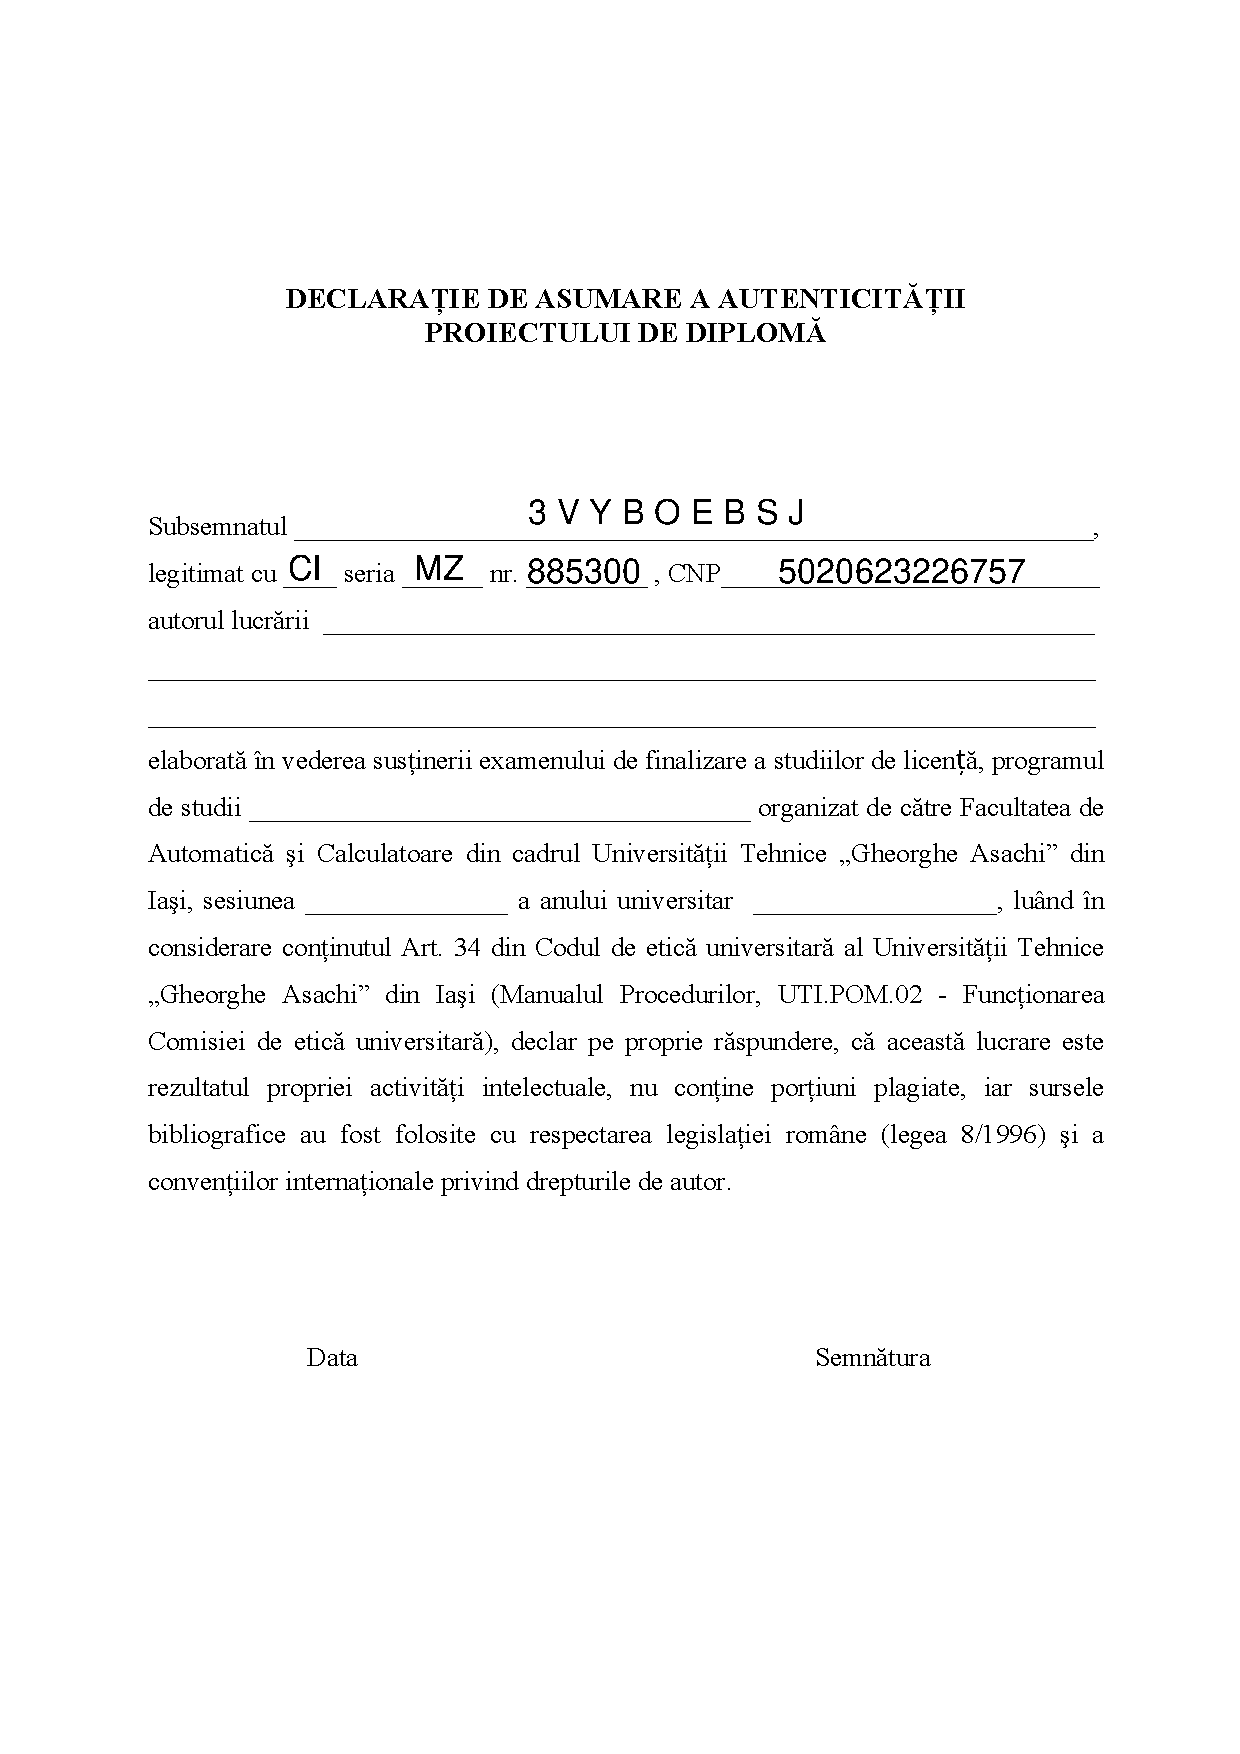
\includepdf[pages=1, scale=1]{pdf/declaratie_autenticitate_diploma_edit}
        % \cleardoublepage
        
        %% cuprins
        \renewcommand{\thispagestyle}[1]{}
        \setcounter{tocdepth}{4}
        \setcounter{secnumdepth}{4}
        \tableofcontents
        \cleardoublepage
        
        %%rezumat
        \newpage
\begin{center}
    \LARGE
    \textbf{\thesistitle}
    
    \vspace{0.5cm}
    
    \authornamefl
    
    \vspace{1cm}
    
    \textbf{Rezumat}
    
    \vspace{1cm}
\end{center}

\textbf{Această secțiune va fi dezvoltată odată cu finalizarea proiectului de licență, cât și a documentației}

Proiectul de diplomă/lucrarea de disertație va conține un scurt rezumat (abstract – termenul în engleză) de maximum o pagină, care expune ideile principale ale tezei, contribuția autorului la realizarea temei propuse precum și concluziile obținute. Formulați ideile principale ale lucrării în propoziții sau fraze cât mai simple, fără amănunte nesemnificative. Încercați să atingeți următoarele idei:
\begin{itemize}
    \item contextul și motivația alegerii temei;
    \item obiectivele principale;
    \item metodologia utilizată;
    \item soluția propusă;
    \item rezultatele esențiale și principalele concluzii.
\end{itemize}

Rezumatul ar trebui să fie între 150-250 de cuvinte și să fie urmat de cuvinte-cheie (\textit{keywords}, 5-7 termeni relevanți).

\textit{Recomandare neoficială: Rezumatul se compune, de obicei, după ce ați terminat redactarea lucrării de licență/disertație, după finalizarea capitolului Concluzii}
        \cleardoublepage
    }
    
    %% reset numerotare pagini
    \setcounter{page}{1}
    \pagenumbering{arabic}
    %% import setari generale
    %% creez o comanda nou pentru capitolele ne-numerotate pentru a le putea prelua in header si a le putea adauga la cuprins;
%% in loc de \chapter*{....} va fi \silentchapter{....}
%% sursa de inspiratie pentru \silentchapter{....}: 
%% https://tex.stackexchange.com/questions/89914/chapter-name-in-the-header-with-chapter
\newcommand{\silentchapter}[1]{
    \chapter*{#1}
    \markboth{#1}{#1}
    \addcontentsline{toc}{chapter}{#1}
}

%% notele de subsol vor fi numerotate in continuu pe parcursul tezei
%% fara a mai fi resetate la fieare capitol
\counterwithout{footnote}{chapter}

%% setarile corespunzatoare antetului/subsolului unei pagini de continut
\pagestyle{fancy}
\fancyhf{}
%% pagina impara
%%      antet: titlul capitolului, aliniat in dreapta
%%      subsol: numarul paginii, aliniat in dreapta
\fancyhead[RO]{\nouppercase \leftmark}
\fancyfoot[RO]{\thepage}
%% pagina para
%%      antet: numele autorului, aliniat in stanga
%%      subsol: numarul paginii, aliniat in stanga
\fancyhead[LE]{\authornamefl}
\fancyfoot[LE]{\thepage}

%% setarile corespunzatoare antetului/subsolului unei pagini de inceput de capitol
%% se defineste prin \fancypagestyle{plain}{...}
\fancypagestyle{plain}{
    \fancyhf{}
    \fancyhead[RO]{\nouppercase \leftmark}
    \fancyfoot[RO]{\thepage}
}

%% definitii culori
\definecolor{albastru-ac}{HTML}{004586}

%% Titlu capitol
%% setari format
\titleformat
    {\chapter}%
    [hang]% titlul pe acelasi rand cu eticheta de capitol
    % bold, dimensiune 14pt (pentru normal 12pt), culoare
    {\color{albastru-ac}\bfseries\large}
    {Capitolul \thechapter.\ }% eticheta capitol
    {0pt}% separator
    {}% before-code -- nu setez nimic
    []% after-code -- nu setez nimic
%% setari spatiere
\titlespacing
    {\chapter}%
    {1.27cm}% aliniere la stanga
    {0.42cm}% spatiu inainte de titlul capitolului
    {0.42cm}% spatiu dupa titlul capitolului
    [0pt]% spatiu fata e marginea din dreapta

%% Subcapitol #.# (\section)
%% modul de lucru este acelasi, nu sunt reluate comentariile
\titleformat
    {\section}
    [hang]
    {\color{albastru-ac}\bfseries\itshape}
    {\thesection.\ }
    {0pt}
    {}
    []
\titlespacing
    {\section}%
    {1.27cm}
    {0.42cm}
    {0.21cm}
    [0pt]

%% Subsubcapitol #.#.# (\subsection)
%% modul de lucru este acelasi, nu sunt reluate comentariile
\titleformat
    {\subsection}
    [hang]
    {\color{albastru-ac}\itshape}
    {\thesubsection.\ }
    {0pt}
    {}
    []
\titlespacing
    {\subsection}%
    {1.27cm}
    {0.42cm}
    {0.21cm}
    [0pt]

%% Subsubsubcapitol #.#.#.# (\subsubsection)
%% modul de lucru este acelasi, nu sunt reluate comentariile
\titleformat
    {\subsubsection}
    [hang]
    {\color{albastru-ac}}
    {\thesubsubsection.\ }
    {0pt}
    {}
    []
\titlespacing
    {\subsubsection}%
    {1.27cm}
    {0.42cm}
    {0.21cm}
    [0pt]

%% configurari caption figura
%% - separator .
%% - dimensiune font 11pt (\small)
%% - culoare albastru (similar capitol)
%% - titlul apare centrat sub figura
\captionsetup[figure]{
    labelsep=period,
    font={small, color=albastru-ac},
    justification=centering,
    position=below
}
%% - numerotarea figurilor se face relativ la capitol (George Vieriu style)
\renewcommand{\thefigure}{\arabic{chapter}.\arabic{figure}}

%% configurari caption tabel
%% - separator .
%% - dimensiune font 11pt (\small)
%% - culoare albastru (similar capitol)
%% - titlul apare centrat deasupra figura
%% - namele intrarii de tabel
\captionsetup[table]{
    labelsep=period,
    font={small, color=albastru-ac},
    justification=centering,
    position=above,
    name=Tabelul
}
%% - numerotarea figurilor se face relativ la capitol (George Vieriu style)
\renewcommand{\thetable}{\arabic{chapter}.\arabic{table}}

%% - numerotarea ecuatiilor se face relativ la capitol (non George Vieriu style)
%% (este modul implicit de lucru)
%% - referirea unei ecuatii se face cu comanda \eqref{label:ecuatie}
%% - numerotarea definitiilor si teoremelor nu este precizata in template-ul lui George Vieriu
%% (din nou, am lasat modul implicit de lucru, si anume, relativ la capitol)
\theoremstyle{definition}
\newtheorem{definition}{Definiția}[chapter]
%% - teoreme
\theoremstyle{plain}
\newtheorem{theorem}{Teorema}[chapter]

%% configurari algoritmi
%% - denumire in romana
\floatname{algorithm}{Algoritmul}
%% - este definita o pseudo-instructiunie pentru "eticheta" de pas in proceduri
\makeatletter
\def\BState{\State\hskip-\ALG@thistlm}
\makeatother

%% configurari listing-uri de cod
%% - pachet minted
%% in loc de \begin{listing} {...} \end{listing} va fi folosit noul environment code: \begin{code} {...} \end{code}
%% ceea ce permite ca \begin{minted} {...} \end{minted} sa fie in interiorul \begin{code} {...} \end{code}
\newenvironment{code}{
    \captionsetup{
        type=listing,
        font={small, color=albastru-ac},
        labelsep=period,
        skip=-0.5em, % mut caption-ul putin mai aproape de cod
    }
}{\vspace{1.5em}}

%% - font pentru numarul liniei din cod
\renewcommand{\theFancyVerbLine}{
    \fontfamily{pcr}\small \arabic{FancyVerbLine}
}

%% setarea globala a optiunilor pentru minted, pentru a nu fi scrise de fiecare data dupa \begin{minted}
\setminted{
    frame=none,
    framesep=1mm,
    linenos=true,
    xleftmargin=1em,
    tabsize=2,
    fontfamily=courier,
    autogobble,
    breaklines,
    fontsize=\small,
    escapeinside=|| %pentru a putea ava cod latex inside minted (referi linii de cod)
}

%% afisare DOI ca link in bibliografie
% - articolele de jurnal/conferinta pot avea un identificator de tip DOI (Digital Object Identifier)
% - in functie de indexarea articolului, aceasta informatie poate fi:
%       - doi.org - in mod uzual pentru jurnale/conferinte indexate ISI
%       - acm.org - pentru jurnale/conferinte indexate ACM
% - in bibliografie, DOI-ul se trece optional in campul "note", 
%   folosind una dintre cele doua comenzi definite mai jos
\newcommand*{\doi}[1]{DOI: \href{https://doi.org/\detokenize{#1}}{\detokenize{#1}}}
\newcommand*{\doiacm}[1]{DOI: \href{https://dl.acm.org/doi/\detokenize{#1}}{\detokenize{#1}}} 

%% break long URL in footnotes
% sursa - Catalin from https://groups.google.com/g/pandoc-discuss/c/Ttvfpz7zTCY?pli=1
\def\UrlBreaks{\do\.\do\@\do\\\do\/\do\!\do\_\do\|\do\%\do\;\do\>\do\]%
\do\)\do\,\do\?\do\'\do\+\do\=\do\#\do\-}%
\Urlmuskip=0mu plus 1mu %
    
    %% *************** continutul efectiv al lucrarii ***************
    %% dupa fiecare capitol, in main.tex este introdus \cleardoublepage pentru ca fiecare capitol nou sa inceapa pe pagina impara
    \chapter{Introducere}
\label{cap:cap1}

Evoluția tehnologică accelerată din ultimele decenii a generat transformări profunde în multiple sectoare ale societății, influențând fundamental modul de acces la informație, furnizarea serviciilor și interacțiunile cotidiene. Aceste progrese au facilitat materializarea unor soluții tehnice care, anterior, erau considerate concepte futuriste. În acest context, tehnologiile de realitate augmentată (AR) și realitate virtuală (VR) s-au conturat ca domenii inovatoare, cu un potențial semnificativ de a reconfigura experiența umană în mediul digital.

În România, deși adoptarea pe scară largă a tehnologiilor AR și VR se află într-un stadiu emergent, parțial condiționată de factori precum costurile echipamentelor specializate și dezvoltarea infrastructurii aferente, perspectivele de aplicabilitate sunt considerabile. Realitatea augmentată și realitatea virtuală permit crearea, controlul și personalizarea avansată a experiențelor digitale, oferind noi paradigme pentru interacțiunea utilizatorului cu conținutul virtual. De la educație și medicină, până la divertisment și turism virtual, aplicațiile realizate în realitatea virtuală sunt aproape nelimitate, în sensul că imaginația este singura limită pe care o avem. În ciuda popularității reduse la nivel local, interesul pentru realitatea virtuală este în creștere, iar odată cu evoluția platformelor ce pot aduce ideile în realitate (Unreal Engine, Unity, Godot, etc.) și integrarea unor tehnologii avansate disponibile la nivel de procesor, procesor grafic și software avansat fac posibilă construirea unor experiențe vizuale fluide, realiste și accesibile unui public tot mai larg.

Lucrarea intitulată „VR Museum” este un program realizat în Unreal Engine, iar împreună cu câteva plugin-uri dezvoltate de Nvidia, reprezintă un muzeu prezentat în realitate virtuală, în care utilizatorul se poate plimba liber printre mai multe exponate, amplasate atât în interiorul muzeului, cât și în exteriorul acestuia. 

Experiența a fost concepută cu scopul de a oferi o lume cât mai apropiată de realitate, dedicată inclusiv persoanelor care nu se pot deplasa fizic într-un muzeu - fie din cauza distanței, a timpului limitat sau a gradului redus de accesibilitate.

Promovând ideea de „cultură la un click distanță”, VR Museum este disponibil gratuit și poate fi descărcat pe orice laptop sau computer care îndeplinește cerințele minime de sistem necesare pentru rulare. Proiectul este unul unic în România în ceea ce privește digitalizarea muzeelor de științe naturale, adresând un gol semnificativ în peisajul local al aplicațiilor educaționale de tip “immersive”.

De asemenea, codul sursă al aplicației (proiectul dezvoltat în Unreal Engine) este disponibil public și poate fi accesat fără niciun cost. Astfel, el poate fi folosit ca o bază, un punct de plecare pentru extinderi ulterioare, integrarea în proiecte mai ample sau ca resursă educațională pentru alți dezvoltatori interesați de tehnologiile VR.

\section{Metodologie}

Această secțiune prezintă metodologia utilizată pentru dezvoltarea aplicației de realitate virtuală „VR Museum”. Sunt detaliate alegerile tehnologice fundamentale, procesul de design și implementare, precum și abordarea privind testarea funcționalității și a experienței utilizatorului. 

Proiectul „VR Museum” a fost dezvoltat utilizând motorul grafic \textbf{Unreal Engine 5.4.4}. Această platformă a fost selectată datorită capabilităților sale avansate în redarea grafică fotorealistă, simularea fizică precisă și suportului extensiv pentru dezvoltarea aplicațiilor de realitate virtuală, aspecte esențiale pentru crearea unei experiențe muzeale de tip "immersive". A fost utilizat un șablon (template) dedicat aplicațiilor VR, care a constituit punctul de plecare, fiind ulterior adaptat specificului proiectului. 

Pentru a atinge un nivel ridicat de fidelitate vizuală și performanță, au fost integrate și configurate manual următoarele tehnologii cheie din Unreal Engine 5: 

\begin{adjustwidth}{2em}{0pt}
\begin{description}
\item[\textbf{Lumen:}] sistemul de iluminare globală și reflexii dinamice a fost utilizat pentru a genera o ambianță luminoasă realistă și interactivă în cadrul spațiilor muzeale, atât interioare, cât și exterioare; 
    
\item[\textbf{Nanite: }] tehnologia de virtualizare a geometriei a permis randarea eficientă a modelelor 3D cu un grad înalt de detaliu (exponate, elemente arhitecturale), fără a compromite semnificativ performanța; 

\item[\textbf{Nvidia DLSS: }] această tehnologie a fost implementată pentru a optimiza rata de cadre pe secundă (FPS), permițând rularea aplicației pe configurații hardware cu plăci video Nvidia diverse, menținând în același timp o calitate vizuală superioară. S-a urmărit astfel o scalabilitate a experienței în funcție de resursele hardware disponibile utilizatorului.
\end{description}
\end{adjustwidth}


\noindent Dezvoltarea aplicației „VR Museum” a urmat un proces iterativ, structurat în următoarele etape principale:

\noindent \textbf{Concepția și proiectarea arhitecturală}

\begin{itemize}
  \item Definirea structurii spațiale a muzeului, incluzând atât zonele interioare de expunere, cât și mediul exterior explorabil. S-a optat pentru o clădire de dimensiuni moderate pentru a optimiza încărcarea resurselor;
  \item Stabilirea layout-ului general și a fluxului de navigare pentru utilizator.
\end{itemize}

\noindent \textbf{Modelarea și crearea mediului virtual}

\begin{itemize}
  \item Realizarea modelului 3D al clădirii muzeului;
  \item Aplicarea texturilor pe suprafețele interioare și exterioare pentru a conferi realism și identitate vizuală;
  \item Dezvoltarea peisajului exterior, care a inclus modelarea terenului, aplicarea texturilor specifice (sol, iarbă) și adăugarea de elemente de vegetație și decorative;
  \item Integrarea resurselor grafice 3D (asset-uri), precum modele de exponate și elemente de decor, provenind din surse online cu licență de utilizare gratuită (ex. Fab Marketplace – Epic Games). Acestea au fost selectate pentru compatibilitatea cu Unreal Engine și relevanța pentru tematica muzeală.
\end{itemize}

\noindent \textbf{Implementarea detaliilor vizuale și funcționale}

\begin{itemize}
  \item Amplasarea și configurarea exponatelor în cadrul muzeului;
  \item Configurarea fină a sistemelor Lumen și Nanite pentru a maximiza calitatea vizuală în raport cu performanța;
  \item Includerea unor obiecte și elemente de scenă menite să valorifice capabilitățile avansate de randare (de ex., prin reflexii detaliate sau interacțiunea luminii cu materiale complexe, specific Ray Tracing-ului implicit sau explicit configurat).
\end{itemize}

Procesul de testare a aplicației „VR Museum” a fost realizat iterativ, pe parcursul întregului ciclu de dezvoltare, pentru a asigura funcționalitatea corespunzătoare și o experiență calitativă pentru utilizator. Aceste teste au fost efectuate utilizând un set de realitate virtuală Oculus Quest 2, conectat la un sistem PC prin multiple configurații:

\begin{itemize}
  \item Conexiune wireless, prin intermediul aplicației Virtual Desktop și al platformei SteamVR;
  \item Conexiune prin cablu, utilizând Oculus Link și runtime-ul OculusXR.
\end{itemize}

\noindent Principalele aspecte urmărite în cadrul testării au fost:

\begin{itemize}
    \item Funcționalitatea de navigare, libertatea de mișcare, coliziunile cu mediul, fluența deplasării.
    \item Calitatea vizuală, corectitudinea afișării texturilor, materialelor, iluminării și a modelelor 3D.
    \item Performanța, menținerea unei rate de cadre constante și acceptabile pentru o experiență VR confortabilă, monitorizarea latenței.
    \item Imersiunea și usabilitatea - evaluarea generală a experienței utilizatorului în mediul virtual.
\end{itemize}


\section{Structura lucrării}

Lucrarea este structurată într-un mod logic și progresiv. La început, sunt prezentate fundamentele teoretice ale tehnologiilor utilizate, continuând apoi cu procesul de dezvoltare a experienței VR Museum.

În primele capitole sunt abordate conceptele de bază legate de realitatea virtuală, detalii despre versiunea Unreal Engine folosită și opțiunile noi pe care aceasta le aduce față de versiunile anterioare. Sunt explicate tehnologiile Lumen, Nanite, Ray Tracing, Path Tracing și DLSS, fiecare având un rol esențial în obținerea unei experiențe vizuale realiste și memorabile.

Ulterior, lucrarea descrie metodologia aplicată în dezvoltarea aplicației, evidențiind soluțiile propuse pentru interacțiune, navigare, implementarea motorului audio (sound engine), precum și setările și optimizările realizate pentru îmbunătățirea performanței aplicației.

De asemenea, sunt menționate pe scurt și componentele predefinite din șablonul oferit de Unreal Engine, care includ funcții esențiale pentru o dezvoltare cât mai simplă și eficientă a funcționalităților specifice realității virtuale.

Lucrarea conține și un capitol dedicat testării aplicației, atât din punct de vedere tehnic (hardware, performanță, recomandări de setări), cât și din perspectiva experienței utilizatorului. Aceasta este analizată atât de către dezvoltatorul aplicației, cât și de alte persoane care au avut ocazia să testeze muzeul virtual și să ofere feedback.

În final, lucrarea se încheie cu o serie de concluzii personale legate de întregul proces de dezvoltare, lecțiile învățate, dificultățile întâmpinate și modul în care au fost soluționate. Sunt prezentate și direcțiile posibile de extindere a proiectului în viitor.

Bibliografia reunește sursele de informare utilizate pe parcursul cercetării, incluzând documentații oficiale, resurse online și lucrări relevante pentru tematica abordată.

    \cleardoublepage

    \chapter{Fundamentarea teoretică și soluții similare}
\label{cap:cap2}

\section{VR / AR}

Realitatea virtuală și-a făcut apariția conceptuală și experimentală pentru prima dată în anul 1968, odată cu dispozitivul creat de Ivan Sutherland și Bob Sproull, considerat primul sistem de afișare „head-mounted” (HMD). Acest sistem era conectat la un calculator mainframe al epocii, care ocupa adesea o întreagă încăpere și era singurul capabil să proceseze și să redea imaginile grafice tridimensionale simple necesare. Dispozitivul HMD în sine era greoi, impunând suspendarea de tavan, fapt ce i-a atras porecla „The Sword of Damocles” și a subliniat limitările hardware considerabile ale acelor timpuri.

\begin{figure}[h!]
    \centering
    \begin{subfigure}{0.49\textwidth}
        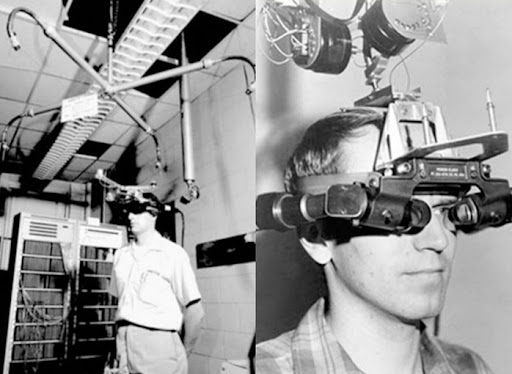
\includegraphics[width=\linewidth, height=6cm]{continut/capitol2/figuri/sword_of_damocles.jpg}
        \caption{The Sword of Damocles}
        \label{fig:sword_of_damocles}
    \end{subfigure}
    \hfill
    \begin{subfigure}{0.49\textwidth}
        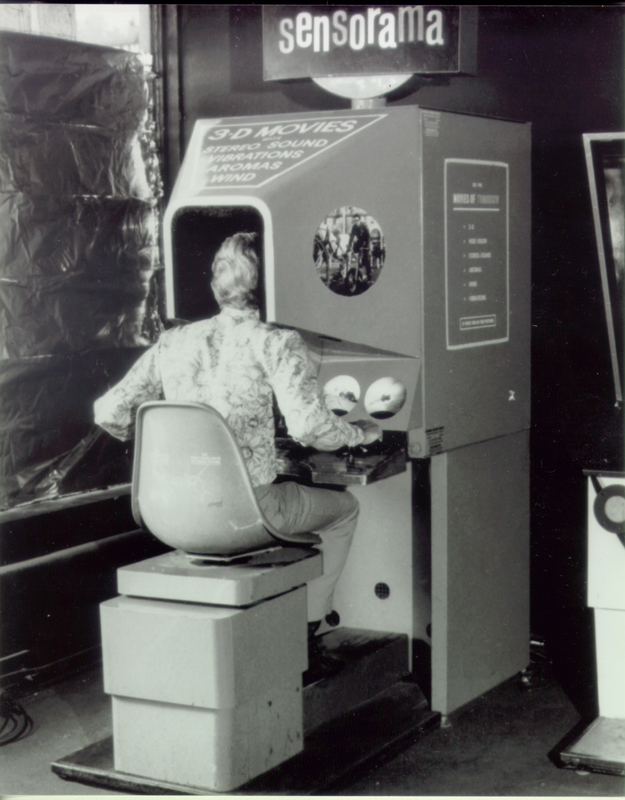
\includegraphics[width=\linewidth, height=6cm]{continut/capitol2/figuri/sensorama.jpg}
        \caption{The Sensorama}
        \label{fig:sensorama}
    \end{subfigure}

    \caption{Istoria VR: Dispozitive timpurii}
    \label{fig:VR_history}
\end{figure}


Desigur, au existat și concepte anterioare acestei inovații. Un exemplu notabil este Sensorama, inventat de Morton Heilig în 1957. Această mașinărie electromecanică voluminoasă funcționa ca o unitate autonomă, integrând toate componentele necesare pentru a oferi o experiență multisenzorială (imagini 3D, sunet stereo, mirosuri, vibrații) pentru până la patru persoane simultan. 
Deși nu era un HMD și nu necesita un calculator extern în sensul modern, Sensorama a reprezentat un precursor important al experiențelor imersive, demonstrând potențialul stimulării multiplelor simțuri.
\begin{wrapfigure}{r}{5cm}
    \centering
    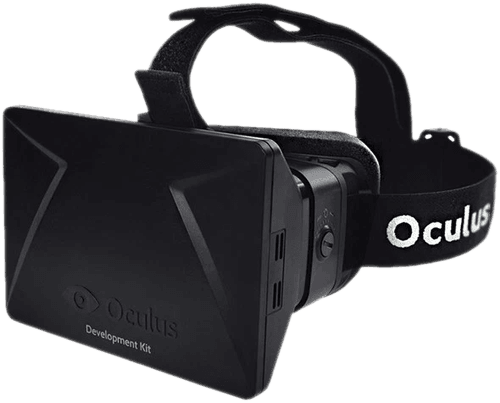
\includegraphics[width=5cm]{continut/capitol2/figuri/oculusriftdk1.png}
    \caption{Oculus Rift DK1}
    \label{fig:Oculus_DK1}
\end{wrapfigure}
Trecerea de la experimente academice la produse orientate către consumatori a fost marcată decisiv de lansarea primului dispozitiv VR fabricat în masă și disponibil publicului larg: Oculus Rift DK1, în martie 2013, la un preț de aproximativ 300 de dolari (aproximativ 450\$ în anul 2025, după calcularea inflației). Apariția sa a fost strâns legată de progresele în tehnologia ecranelor compacte de înaltă rezoluție (impulsionate de industria telefoanelor mobile) și, crucial, de creșterea exponențială a puterii de calcul și accesibilității computerelor personale (PC-urilor). 
Aceste PC-uri, echipate cu plăci grafice din ce în ce mai performante, au devenit platforma hardware necesară pentru a rula aplicațiile VR. Kitul de dezvoltare Oculus Rift DK1 oferea un ecran de 7 inch (1280x800 px, rezultând 640x800 px per ochi), un câmp vizual de aproximativ 90 de grade și un sistem de urmărire a mișcării capului pe trei axe (head-tracking). Deși nu oferea urmărire a poziției în spațiu (positional tracking), care a devenit un standard ulterior și a necesitat dezvoltarea unor sisteme de senzori suplimentari (externi sau integrați), DK1 a reprezentat un moment cheie în popularizarea realității virtuale.
De atunci, evoluția hardware-ului VR a continuat într-un ritm alert.
Dispozitivele ulterioare au adus îmbunătățiri semnificative: rezoluții mult mai mari ale ecranelor, câmpuri vizuale extinse, rate de reîmprospătare superioare, sisteme de urmărire pozițională din ce în ce mai precise (inside-out tracking, eliminând nevoia senzorilor externi), și controlere dedicate cu feedback haptic. În paralel, cerințele hardware pentru PC-urile capabile să susțină aceste experiențe au rămas ridicate, dar au apărut și soluții alternative: console de jocuri cu suport VR și, mai recent, dispozitive VR autonome (standalone), care integrează unitatea de procesare direct în cască, eliminând dependența de un PC sau o consolă externă.

Fie că vorbim despre un dispozitiv VR lansat recent sau unul istoric, principiul de funcționare a rămas același: simularea unei alte realități prin intermediul unor afișaje dedicate pentru fiecare ochi, însoțite de sunet stereo sau 3D, livrat prin căști sau boxe speciale. Cu ajutorul acestor elemente hardware esențiale, simțurile noastre sunt „păcălite” să creadă că ne aflăm într-un alt spațiu, în afara realității imediate, oferind o senzație intensă de imersiune.

\section{Unreal Engine 5}

Fiind succesorul lui Unreal Engine 4, Unreal Engine 5 (UE5) este un motor de joc („game engine”) care permite realizarea unor experiențe interactive de ultimă generație, fiind mult mai ușor de folosit decât dezvoltarea unui engine de la zero. Punctul de plecare este același pentru toți dezvoltatorii, însă UE5 oferă o infinitate de direcții și domenii spre care aceștia se pot orienta. În majoritatea cazurilor sunt create jocuri, dar există și numeroase exemple extra-ludice în care motorul este extrem de util.

\begin{figure} [htp] 
\centering 
\includegraphics [width=12cm]
{continut/capitol2/figuri/ue5.png} 
\caption{Unreal Engine 5 - Deschiderea proiectului} 
\label{fig:VR} 
\end{figure}


Spre exemplu, BMW, Audi, Porsche și Volvo folosesc Unreal pentru dezvoltarea de simulări și prezentări interactive în showroom-uri virtuale: testează noile modele în medii digitale, simulează experiența de condus și rafinează designul auto. Scene din serialul The Mandalorian sau din demonstrația tehnologică The Matrix Awakens se bazează pe UE5 pentru efecte speciale și decoruri realiste, economisind astfel cheltuieli semnificative legate de recuzită fizică.

Versiunea majoră 5.0 (lansată pe 5 aprilie 2022) a adus numeroase îmbunătățiri - Nanite (sistem de geometrie pe bază de micro-poligoane), Lumen (iluminare globală și reflexii în timp real), Ray Tracing avansat, optimizări de performanță și flux de lucru, suport extins pentru MetaHuman și un sistem modernizat de animație și simulare fizică.

Noutățile din 5.4 (folosită în proiectul VR Museum):

\begin{adjustwidth}{2em}{0pt}
\begin{description}
    \item[\textbf{Suport VR/AR unificat prin OpenXR: }] În locul mai multor plugin-uri specifice (de ex. Oculus Plugin pentru Meta Quest), OpenXR oferă un cadru universal compatibil cu majoritatea headset-urilor, reducând timpul de configurare a aceleiași scene pe platforme diferite.
    \item[\textbf{{World Partition: }}] Permite împărțirea lumii în sectoare încărcate și descărcate dinamic, optimizând proiectele cu hărți mari și îmbunătățind performanța editorului și a build-ului final.
    \item[\textbf{{Motion Matching \& animație dinamică avansată: }}] Motorul înțelege mult mai bine părțile corpului și tranzițiile lor, facilitând crearea de animații realiste într-un timp redus. Tehnologia folosește o bază de date de mișcări care sunt selectate și combinate automat în funcție de contextul de gameplay.
\end{description}
\end{adjustwidth}

\section{Ray Tracing}

În jocurile de acum câțiva ani se foloseau diverse tehnici de calculare a luminii. De obicei, lumina era atașată unor obiecte definite drept „light objects”. Parcursul razei era trasat de la punctul A (obiectul emitent) până la punctul B (primul obstacol — un perete ori alt obiect 3D). Din punct de vedere vizual, această metodă tradițională arată în continuare foarte bine datorită optimizărilor și evoluției algoritmilor de rasterizare; totuși, din perspectiva realismului există limite evidente.

Aici intervine Ray Tracing-ul în timp real. Spre deosebire de metodele clasice, tehnica simulează comportamentul fizic al luminii din lumea reală:

\begin{itemize}
    \item Lumina pornește din sursa emitentă în toate direcțiile.
    \item Razele se reflectă, refractă sau sunt absorbite diferit, în funcție de proprietățile fiecărui material (culoare, rugozitate, indice de refracție).
    \item Obiectele din scenă sunt iluminate atât direct (de la sursa primară), cât și indirect (prin reflexii multiple sau lumină difuză), creând umbre moi, reflexii precise și o iluminare globală mai verosimilă.
\end{itemize}

Tehnologia Ray Tracing nu este nouă; ea este folosită de mult timp în cinematografie, mai ales în filmele de animație 3D produse de studiouri precum Pixar, DreamWorks sau Disney. În producția de film, fiecare cadru poate fi randat în minute ori chiar ore pe multe servere, unde costul nu este constrâns de cerințe de timp real. Din acest motiv, tehnica era considerată impracticabilă pentru jocurile video: hardware-ul existent putea livra doar 2–5 cadre pe secundă în condiții optime, mult sub pragul necesar pentru un gameplay fluent.


\section{Evoluția hardware}

Acest lucru s-a schimbat în anul 2018, când Nvidia a lansat prima serie de plăci video ce pot simula lumina în timp real, seria RTX 20. Aceste placi video aveau cateva imbunatatiri fata de seria precedenta, GTX 16: Noi nuclee RT făcute special pentru Ray Tracing, nuclee Tensor pentru DLSS, mult mai multe nuclee CUDA, memorie mai rapidă și shadere Mesh, folosite pentru a susține geometrie mult mai avansată și complexă fără a pierde din perfomanta.

În mod normal, un joc (sau în cazul nostru, o experiență VR) trebuie să ruleze cu peste 30 fps pentru claritate și cu peste 60 fps pentru o experiență cu adevărat plăcută ochilor. Abia odată cu apariția plăcilor grafice cu nuclee dedicate pentru ray tracing și a tehnicilor de upscaling inteligente (DLSS, FSR) a devenit posibilă integrarea ray tracing-ului în timp real, păstrând totodată un număr suficient de cadre pe secundă pentru jocuri moderne.

\section{\textbf{D}eep \textbf{L}earning \textbf{S}uper \textbf{S}ampling}

Prescurtat DLSS și avand 4 versiuni în momentul actual, acest algoritm folosește nucleele Tensor pentru a spori calitatea imaginii. jocul este randat la o rezolutie mai mica, iar placa video tehnologia DLSS pentru a face “upscaling” la imagine, astfel permitandu-ne sa jucam la setari grafice mult mai mari și desigur, cu Ray Tracing pornit.

Cele patru mari generații sunt: 

\begin{center}
\begin{tabular}{||c c c||} 
 \hline
 Versiune & Anul lansării & Noile funcții introduse \\ [0.5ex] 
 \hline\hline
 DLSS 1.0 & 2018 & Super-Sampling AI clasic \\ 
 \hline
 DLSS 2.0 & 2020 & Super Temporal Resolution \\
 \hline
 DLSS 3 & 2022 & Frame Generation, cadre AI pe seria RTX 40 \\
 \hline
 DLSS 4 & 2025 & Multi Frame Generation, mai multe cadre AI generate \\ [1ex] 
 \hline
\end{tabular}
\end{center}

\noindent Între acestea, DLSS 3.5 (2023) a adus „Ray Reconstruction”, un nou model AI care înlocuiește denoiser-ele clasice pentru reflexii și iluminare ray-traced. 

Prima evoluție s-a intamplat în anul 2020 când Nvidia a lansat seria de plăci video RTX 30, unde și-a făcut apariția DLSS 2. Acesta nu numai ca este mult mai eficient și antrenat pe un model mai performant, ci are 4 noi setari: 

\begin{center}
\begin{tabular}{||c c||} 
 \hline
 Calitatea DLSS & Rezoluția internă (procent) \\ [0.5ex] 
 \hline\hline
 Ultra Performance & 33\% (Introdus in DLSS 2.1) \\ 
 \hline
 Performance & 50\%  \\
 \hline
 Balanced & 58\% \\
 \hline
 Quality & 66.6\%  \\ [1ex] 
 \hline
 Native Upscale & 100\% (DLAA, introdus in DLSS 2.2)  \\ [1ex] 
 \hline
\end{tabular}
\end{center}


 În 2022, odată cu seria GeForce RTX 40, DLSS 3 a extins aceste moduri cu Frame Generation, multiplicând rata de cadre cu 2-3× pe titluri compatibile (de ex. Cyberpunk 2077 RT Overdrive). În 2025, DLSS 4 duce mai departe ideea prin Multi Frame Generation, generând până la 8× mai multe cadre la 4K pe RTX 5090, cu un nou model transformator ce îmbunătățește stabilitatea temporală și reduce ghosting-ul. 

Dacă jocul este randat la 1080p (1920×1080), rezoluția reală înainte de acest “upscale” realizat de DLSS sunt următoarele: 

\begin{center}
\begin{tabular}{||c c||} 
 \hline
 Calitatea DLSS & Rezoluția internă \\ [0.5ex] 
 \hline\hline
 Ultra Performance & 640×360 \\ 
 \hline
 Performance & 960×540  \\
 \hline
 Balanced & 1114×626 \\
 \hline
 Quality & 1280×720  \\ [1ex] 
 \hline
 Native Upscale & 1920x1080 \\ [1ex] 
 \hline
\end{tabular}
\end{center}


\noindent Aspectual, deși jocul este la o rezoluție mult mai mică, nu arată foarte diferit față de rezoluția “native”, atunci când nu ar fi fost folosit DLSS. Singurele diferențe se pot remarca la modurile Ultra Performance și Performance la mișcări bruște ale camerei, în special când ne uitam la margini (ex: frunzele din copaci în raport cu cerul, etc.)

DLSS păstrează aceeași factori de scalare pentru 1440p și 4K, iar Ray Reconstruction (DLSS 3.5+) poate diminua artefactele de la margini în scene ray-traced, chiar și în modurile cu rezoluție internă foarte mică. De asemenea, tehnologia poate fi combinată cu NVIDIA Reflex pentru a reduce latența de intrare la sub 10 ms în titluri competitive.

\section{Nanite}

Tehnologia Nanite a fost lansată în anul 2020 împreună cu Unreal Engine 5. Aceasta permite scene vizuale mult mai detaliate, fără a afecta performanța. Dacă pană atunci developerii erau nevoiți sa optimizeze manual numărul de poligoane ce alcătuiau obiectele, după apariția noii tehnologii nu a mai fost necesar. 

Cu Nanite, obiectele, texturile, nivelul de detaliu este ajustat dinamic în funcție de distanța jucătorului pana la obiect, unghiul vizual și puterea de procesare a calculatorului. Astfel, pe ecran va fi reprezentat exact nivelul necesar de poligoane, nu mai mult, nici mai puțin.

\section{Lumen}

Apărut odată cu Unreal Engine 5 și cu Nanite, tehnologia Lumen simuleaza lumina în timp real prin folosirea unor tehnici foarte optimizare.

\textbf{Care este diferenta intre Lumen și Ray Tracing?}

Spre deosebire de Ray Tracing ce folosește nucleele RT pentru procesarea luminii, tehnologia Lumen folosește o combinație dintre \textbf{Voxel Cone Tracing}, \textbf{Global Illumination} si \textbf{Screen Space Reflections} (sau prescurtat SSR) pentru a face posibilă utilizarea și pe un hardware de nivel mediu. 

\begin{adjustwidth}{2em}{0pt}
\begin{description}
    \item[\textbf{Voxel Cone Tracing:}] scena este convertită într-un set de voxels. Acestea se aseamănă cu pixelii, însă în loc de o reprezentare de culoare pe un  plan bidimensional, aceste voxels sunt realizate în spațiul 3D și au mai multe proprietăți (densitate, transparenta, etc.) 
    \item[\textbf{Global Illumination:}] Folosește metoda Ray Tracing pentru a reprezenta un ambient cat mai similar cu lumea reala in ceea ce privește trasarea razelor de lumina.
    \item[\textbf{Screen Space Reflections:}] tehnologie folosită tradițional, nu foarte costisitoare, unde reflexia era generată în funcție de conținutul pe ecran. In general folosita pe suprafete mari (spre exemplu apa), aceasta nu era foarte costisitoare, însă se putea observa cu usurinta folosirea acestei tehnologii prin mișcarea unghiului camerei.
\end{description}
\end{adjustwidth}

\noindent Lumen poate fi folosit și cu Ray Tracing la nivel hardware, pentru un nivel de detaliu mai avansat fără a afecta performanța atat de mult fata de Ray Tracing standard.







\section{Soluții și proiecte asemănătoare}

Dacă ne uităm la exemple din afara țării, putem identifica câteva soluții mai mult sau mai puțin asemănătoare cu VR Museum.

Unul dintre cele mai cunoscute este Google Arts \& Culture, lansat în 2011, un proiect ambițios care oferă tururi virtuale ale peste 500 de muzee din întreaga lume. Experiența este disponibilă atât pe web, cât și în aplicații mobile, iar unele dintre muzeele prezentate sunt compatibile cu dispozitive VR pentru telefon, cum ar fi Google Cardboard. Interacțiunea este însă limitată la explorare vizuală prin imagini 360°, fără posibilități avansate de interacțiune cu obiectele sau mediul.

Un alt exemplu relevant este The Glass Drawing Room – Corning Museum of Glass. Acest proiect, realizat în Unity și inspirat de viziunea arhitectului Robert Adam, recreează în VR o cameră de desen din secolul al XVIII-lea. Sunt puse în evidență detalii precum oglinzile, panourile decorative din sticlă și atmosfera generală a epocii. Aplicația este disponibilă gratuit pentru descărcare.

De asemenea, proiectul Digital Homecoming, realizat de Technology Research Institute for Culture \& Heritage (TRIC), folosește Unreal Engine, același motor grafic utilizat și în dezvoltarea VR Museum. Proiectul creează replici digitale ale artefactelor culturale coreene și le prezintă în expoziții interactive, accesibile publicului din Coreea de Sud și Statele Unite ale Americii. Acesta evidențiază potențialul realității virtuale în conservarea și promovarea patrimoniului cultural.

\section{Cum se construiește o experiență virtuală?}

În ceea ce privește o experiență de tip Virtual Reality, aceasta poate fi realizată în mai multe moduri, în funcție de buget, nivelul dorit de interactivitate și scopul aplicației.

Cea mai accesibilă variantă implică utilizarea unui telefon mobil introdus într-un set de ochelari VR pasivi (precum Google Cardboard), care măresc ecranul telefonului și oferă o experiență de vizualizare 360°. Din păcate, această metodă oferă un control limitat și un nivel redus de realism, fără interacțiune reală cu mediul virtual.

La polul opus, cea mai performantă variantă implică utilizarea unui headset VR dedicat, dotat cu ecran pentru fiecare ochi și controlere pentru interacțiune (ex: Meta Quest 2, folosit și în cadrul acestui proiect). Aceste dispozitive permit urmărirea poziției capului și a mâinilor, oferind o experiență complet imersivă și interactivă.

Realizarea unui astfel de proiect necesită însă timp, experiență și, de cele mai multe ori, o echipă de dezvoltare, pentru a putea livra o aplicație la un nivel consumer-ready. De aceea, multe aplicații VR comerciale sunt disponibile contra cost. În schimb, în mediul educațional și științific, proiectele sunt adesea gratuite, pentru a asigura accesul larg la informații.

Aplicațiile VR pot fi clasificate în mai multe categorii:

\begin{adjustwidth}{2em}{0pt}
\begin{description}
    \item[\textbf{Experiențe 360°}] - bazate pe fotografii sau videoclipuri sferice, unde utilizatorul se poate uita în jur, dar nu poate interacționa sau deplasa;    
    \item[\textbf{Experiențe interactive}] - unde utilizatorul se poate mișca liber în spațiul virtual și poate interacționa cu obiectele din jurul său.
\end{description}
\end{adjustwidth}

\noindent În ceea ce privește nivelul de realism grafic, aplicațiile VR pot fi împărțite în două mari categorii:

\begin{adjustwidth}{2em}{0pt}
\begin{description}
    \item[\textbf{Experiențe cu grafică simplificată}] - create cu resurse reduse (adesea în Unity sau pe console standalone);   
    \item[\textbf{Experiențe avansate}] conectate la un PC cu placă grafică dedicată, unde procesarea este realizată pe computer, iar imaginea este transmisă către headset-ul VR prin cablu sau wireless.
\end{description}
\end{adjustwidth}

\noindent VR Museum face parte din a doua categorie: aplicația este randată pe un laptop sau PC performant, folosind puterea unei plăci grafice dedicate (ex. Nvidia RTX), iar imaginea este transmisă către headset folosind un runtime compatibil. În ciuda nivelului grafic ridicat și al tehnologiilor avansate integrate, aplicația este disponibilă gratuit, cu condiția ca utilizatorul să dețină un sistem compatibil care să susțină performanțele necesare.

\section{Conceptul de realitate virtuală în România}

În România, astfel de proiecte sunt aproape inexistente, iar cauzele sunt multiple. În multe cazuri, muzeele fizice abia reușesc să fie renovate sau menținute funcționale, așa că ideea unor versiuni virtuale pare, cel puțin deocamdată, prematură - sau chiar utopică. Unele muzee nu arată bine nici în realitate, darămite într-o experiență VR – un aspect poate amuzant, dar realist.

Un exemplu pozitiv este Muzeul Antipa din București, care este bine organizat și modernizat, însă nu dispune de o versiune virtuală. Asta în ciuda faptului că infrastructura sa ar permite o digitalizare de calitate. 
Din păcate, în România, tehnologia evoluează mai lent, iar dispozitivele VR sunt costisitoare, devenind inaccesibile pentru o mare parte a populației. Acest context explică de ce astfel de aplicații nu sunt încă dezvoltate la nivel local.

Un alt obstacol frecvent întâlnit este reprezentat de cerințele hardware ridicate sau neclare, care pot pune probleme utilizatorilor cu sisteme clasificate ca fiind „mid-range”. Multe aplicații VR nu sunt optimizate pentru a funcționa eficient pe configurații accesibile, necesitând plăci grafice puternice și procesoare performante.

Proiectul VR Museum vine să umple acest gol din peisajul educațional românesc printr-o abordare modernă, accesibilă și scalabilă. După cum a fost menționat anterior, aplicația este gratuită și poate fi testată de mai mulți utilizatori, chiar dacă se folosește un singur laptop sau PC performant. Folosește cele mai recente tehnologii grafice, precum Ray Tracing, DLSS și Nanite, oferind o experiență cu mișcare liberă și interacțiune realistă într-un mediu virtual.

În plus, VR Museum este un proiect open-source, ceea ce înseamnă că poate fi extins și adaptat de către alți dezvoltatori interesați. Poate servi ca bază pentru lucrări viitoare, proiecte educaționale sau chiar inițiative culturale locale. Faptul că nu impune nicio restricție comercială îl face o soluție ideală pentru scopuri didactice și explorare creativă.

\section{Așteptări de la proiectul de licență VR Museum}

În continuare sunt prezentate specificațiile funcționale și tehnice propuse pentru aplicația VR Museum, cu scopul de a ghida dezvoltarea acesteia și de a asigura o experiență interactivă, realistă și accesibilă.

Experiența este concepută cu un grad ridicat de accesibilitate, astfel încât oricine să se poată bucura de ea, indiferent de nivelul de experiență cu tehnologia VR. Aplicația este destinată publicului larg, în special elevilor, studenților sau vizitatorilor care, din diverse motive, nu pot accesa fizic un muzeu real.

VR Museum trebuie să ruleze fluent pe un sistem mid-range, fiind optimizată pentru plăci video din seria Nvidia RTX 20 si mai noi, în combinație cu 16 GB RAM și un procesor cu minimum șase nuclee. Experiența VR este posibilă prin utilizarea unui set de ochelari de realitate virtuală, conectat la desktop sau laptop prin cabluri dedicate (Oculus Link) sau prin conexiune wireless (ex: Virtual Desktop, Air Link).

Utilizatorul se poate deplasa liber în mediul virtual, folosind controlerele (manetele) headset-ului. Mișcarea este concepută să fie naturală și confortabilă, pentru a minimiza disconfortul asociat (ex. motion sickness). Navigarea se realizează intuitiv, prin joystick sau teleportare, în funcție de preferințe.

Aplicația include un sistem de sunet spațial (3D), menit să amplifice nivelul de imersiune, atât prin efecte ambientale (pași, ecou, zgomote de fundal), cât și prin sunete declanșate în urma interacțiunii directe cu exponatele.

Structura aplicației este modulară, ceea ce permite adăugarea de noi camere, teme, hărți, exponate sau pachete audio, fără a fi necesară rescrierea arhitecturii de bază. Proiectul este gândit să fie accesibil și ușor de extins, indiferent dacă este abordat de un dezvoltator începător sau unul cu experiență, fiind o bază solidă pentru proiecte educaționale viitoare.
    \cleardoublepage

    \chapter{Soluția propusă}
\label{cap:cap3}

\section{Problema națională a departamentului}

În România, lipsește orice formă de integrare virtuală a muzeelor, fie că vorbim despre cele de științe naturale, istorice, de artă sau alte tipuri. Pe lângă acest aspect, se remarcă și o lipsă semnificativă a infrastructurii necesare pentru dezvoltarea unor astfel de proiecte, cauzată de mai mulți factori: limitări financiare, lipsa de timp, nivelul redus de familiarizare cu astfel de tehnologii, sau dificultatea implementării în medii instituționale.

Cu toate acestea, tehnologia evoluează constant, iar momentul actual este propice pentru o schimbare în acest sens – în special în context educațional, unde digitalizarea devine tot mai importantă.

Proiectul VR Museum propune o alternativă modernă și accesibilă, oferind o experiență de vizitare virtuală a unui muzeu de științe naturale. Aplicația este gratuită, singura condiție fiind deținerea unui sistem compatibil VR (laptop sau desktop performant, conectat la un headset VR).

Proiectul este ușor de extins și adaptat, fiind open-source și accesibil pentru oricine dorește să contribuie – fie dezvoltatori aflați la început de drum, fie utilizatori avansați care doresc să adauge funcționalități sau conținut suplimentar.

VR Museum utilizează cele mai noi tehnologii disponibile în prezent, fiind realizat în Unreal Engine 5.4.4. Acesta beneficiază de o arhitectură modulară, în care fiecare componentă (scene, sunet, interacțiuni, meniu, logică etc.) este tratată separat, permițând dezvoltarea și testarea independentă a fiecărui element. Astfel, aplicația poate evolua rapid, fără a necesita refacerea completă a codului sau a scenei.

\section{Categorii de proiecte în Unreal Engine 5}

\begin{figure} [htp] 
\centering 
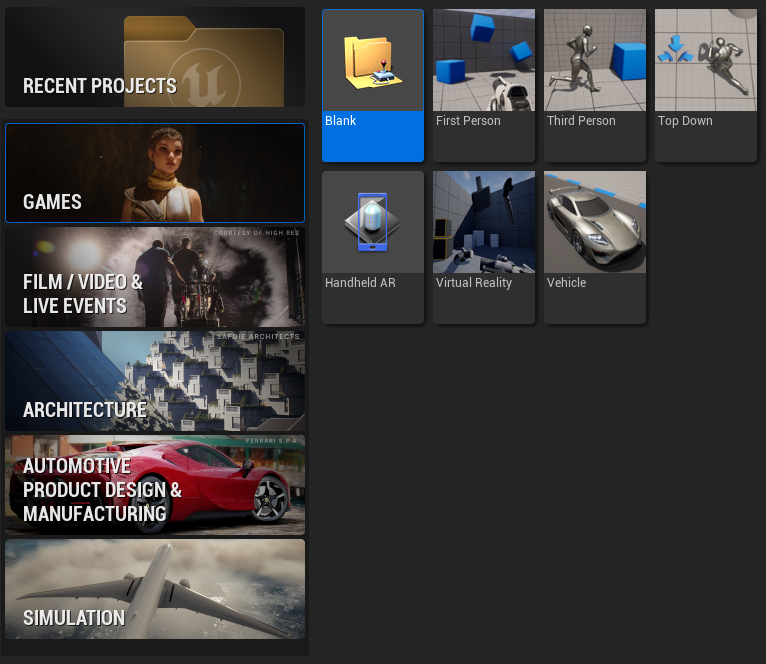
\includegraphics [width=12cm]
{continut/capitol3/figuri/UE_Templates.png} 
\caption{Proiecte de tip "template"} 
\label{fig:VR_Templates} 
\end{figure}

Un proiect în Unreal Engine 5 începe prin alegerea unui șablon de bază, organizat în funcție de scopul aplicației. Motorul oferă o serie de categorii predefinite care acoperă o gamă largă de domenii, de la dezvoltarea de jocuri până la aplicații industriale și vizualizari arhitecturale. 

\begin{itemize}
\item \textbf{Games} - este utilizată în principal pentru dezvoltarea de jocuri video și experiențe interactive. Aceasta a fost și opțiunea selectată pentru proiectul de față - VR Museum - datorită flexibilității și compatibilității cu template-ul „Virtual Reality”. Majoritatea dezvoltatorilor din industria de gaming aleg această categorie pentru prototipuri și produse finale. Jocuri comerciale de renume precum Fortnite, Valorant sau Poppy Playtime sunt exemple concrete ale utilizării Unreal Engine în producția de jocuri ”AAA” sau ”Indie”.
\item \textbf{Film / Video \& Live Events} - crearea de efecte vizuale și medii digitale pentru producții cinematografice sau evenimente live poate fi extrem de costisitoare, mai ales când se folosesc decoruri reale. Unreal Engine oferă instrumente avansate pentru previzualizare, in-camera VFX și integrare cu LED volume, reducând astfel costurile de producție și timpul de execuție. Un exemplu notabil este utilizarea Unreal Engine în realizarea unor secvențe din serialul ”The Mandalorian” (Star Wars), unde fundalurile generate în timp real au înlocuit decorurile tradiționale.
\item \textbf{Architecture} - categoria dedicată arhitecturii permite crearea de vizualizări realiste pentru proiecte de construcții și design interior. Aceasta oferă integrare nativă cu instrumente CAD și BIM (precum Revit, ArchiCAD), prin intermediul Datasmith. Se pot crea schițe interactive, simulări de iluminare naturală și tururi virtuale, facilitând colaborarea dintre arhitecți, designeri și clienți. Această abordare reduce riscul de erori și crește eficiența în procesul decizional.
\item \textbf{Automotive Product Design \& Manufacturing} - este conceput special pentru industria auto, acoperind atât partea de vizualizare a designului vehiculului, cât și prototiparea interfețelor grafice utilizate în habitaclu (HMI - Human-Machine Interface). De exemplu, Mercedes-Benz utilizează Unreal Engine în dezvoltarea interfeței digitale MBUX Hyperscreen, un sistem avansat care rulează pe un ecran panoramic. De asemenea, General Motors integrează Unreal în platforma Ultium, utilizată în vehicule electrice precum Cadillac și Hummer EV, pentru a genera în timp real animații și interacțiuni în bordul mașinii.
\item \textbf{Simulation} - destinată dezvoltării de simulatoare pentru aplicații educaționale, industriale sau de formare profesională. Unreal Engine permite integrarea fizicii avansate, a senzorilor virtuali și a scenariilor dinamice. Aceasta este utilizată, de exemplu, pentru simulatoare de zbor, simulatoare auto (pentru camioane, trenuri etc.) sau pentru programe de instruire în medii controlate, precum aplicațiile medicale sau militare. Realismul oferit de motorul grafic contribuie la crearea unor experiențe imersive și credibile, utile în formarea personalului specializat.

\end{itemize}

Categoria Games din Unreal Engine 5 este destinată proiectelor interactive, în special jocurilor video. Ea oferă mai multe șabloane (templates) predefinite care acoperă diverse tipuri de gameplay și stiluri de joc. Alegerea unui template potrivit poate accelera procesul de prototipare și dezvoltare, oferind o bază funcțională adaptată nevoilor proiectului. Dintre acestea, cele mai utilizate sunt:

\begin{itemize}
\item \textbf{Blank} - oferă un proiect complet gol, fără personaje, logică de joc sau componente suplimentare. Este potrivit pentru dezvoltatori care doresc să construiască o experiență complet personalizată, de la zero, fără a fi constrânși de o structură predefinită.
\item \textbf{First Person} - este utilizat pentru jocuri de tip shooter sau explorare. Include un personaj preconfigurat, cu posibilitatea de a interacționa cu obiecte, a sări și a trage cu un proiectil. Un exemplu de joc popular dezvoltat în Unreal Engine care folosește perspectiva first person este Poppy Playtime.
\item \textbf{Third Person} - include un personaj văzut din spate și o cameră cinematică de urmărire. Este frecvent utilizat în jocuri narative sau de aventură. Un exemplu relevant este Tomb Raider (Shadow of the Tomb Raider), dezvoltat parțial folosind Unreal Engine, care utilizează această perspectivă pentru a crea o experiență dinamică.
\item \textbf{Top Down} - presupune o cameră plasată deasupra personajului, ideal pentru jocuri tactice, RPG-uri sau strategie în timp real. Exemple de astfel de jocuri sunt Transistor și The Ascent, care adoptă această perspectivă pentru a oferi o viziune strategică asupra mediului.
\item \textbf{Handheld AR} - orientat spre aplicații de realitate augmentată (AR) pe dispozitive mobile. Permite recunoașterea planurilor reale și plasarea obiectelor 3D în spațiul fizic. Exemple de aplicații similare includ Pokémon GO, Minecraft Earth, sau funcționalitatea View in 3D/AR oferită de Google Search, unde utilizatorii pot vizualiza animale, obiecte sau produse în propriul mediu, prin camera telefonului.
\item \textbf{Vehicle} - conține o logică de conducere a unui vehicul cu roți și suspensii fizice. Este folosit în dezvoltarea jocurilor de tip racing sau simulatoare de condus. Printre exemplele celebre se numără GRIP: Combat Racing sau Next Car Game: Wreckfest, care folosesc componente fizice avansate pentru a simula comportamentul realist al vehiculelor.
\item \textbf{Virtual Reality (VR)} - acest template este special conceput pentru dezvoltarea de aplicații în realitate virtuală, compatibil cu standardul OpenXR. Include funcționalități precum teleportarea, interacțiunea cu obiecte (grab), meniuri 3D și suport pentru modul spectator. În cadrul lucrării de licență, acest template a fost ales ca punct de plecare pentru realizarea aplicației VR Museum. Detaliile tehnice și funcționale ale acestui șablon vor fi prezentate în secțiunile următoare.

\end{itemize}

\section{Structura și funcționalitățile șablonului VR Template}

Șablonul Virtual Reality Template oferit de Unreal Engine 5 este un punct de plecare extrem de util pentru dezvoltatorii care doresc să creeze experiențe imersive în realitate virtuală. Acesta vine preconfigurat cu o serie de funcționalități esențiale pentru interacțiunea naturală în medii tridimensionale, permițând un timp de dezvoltare redus și o adaptabilitate ridicată pentru diverse tipuri de proiecte VR.

\begin{figure}[h!]
    \centering
    \begin{subfigure}{0.49\textwidth}
        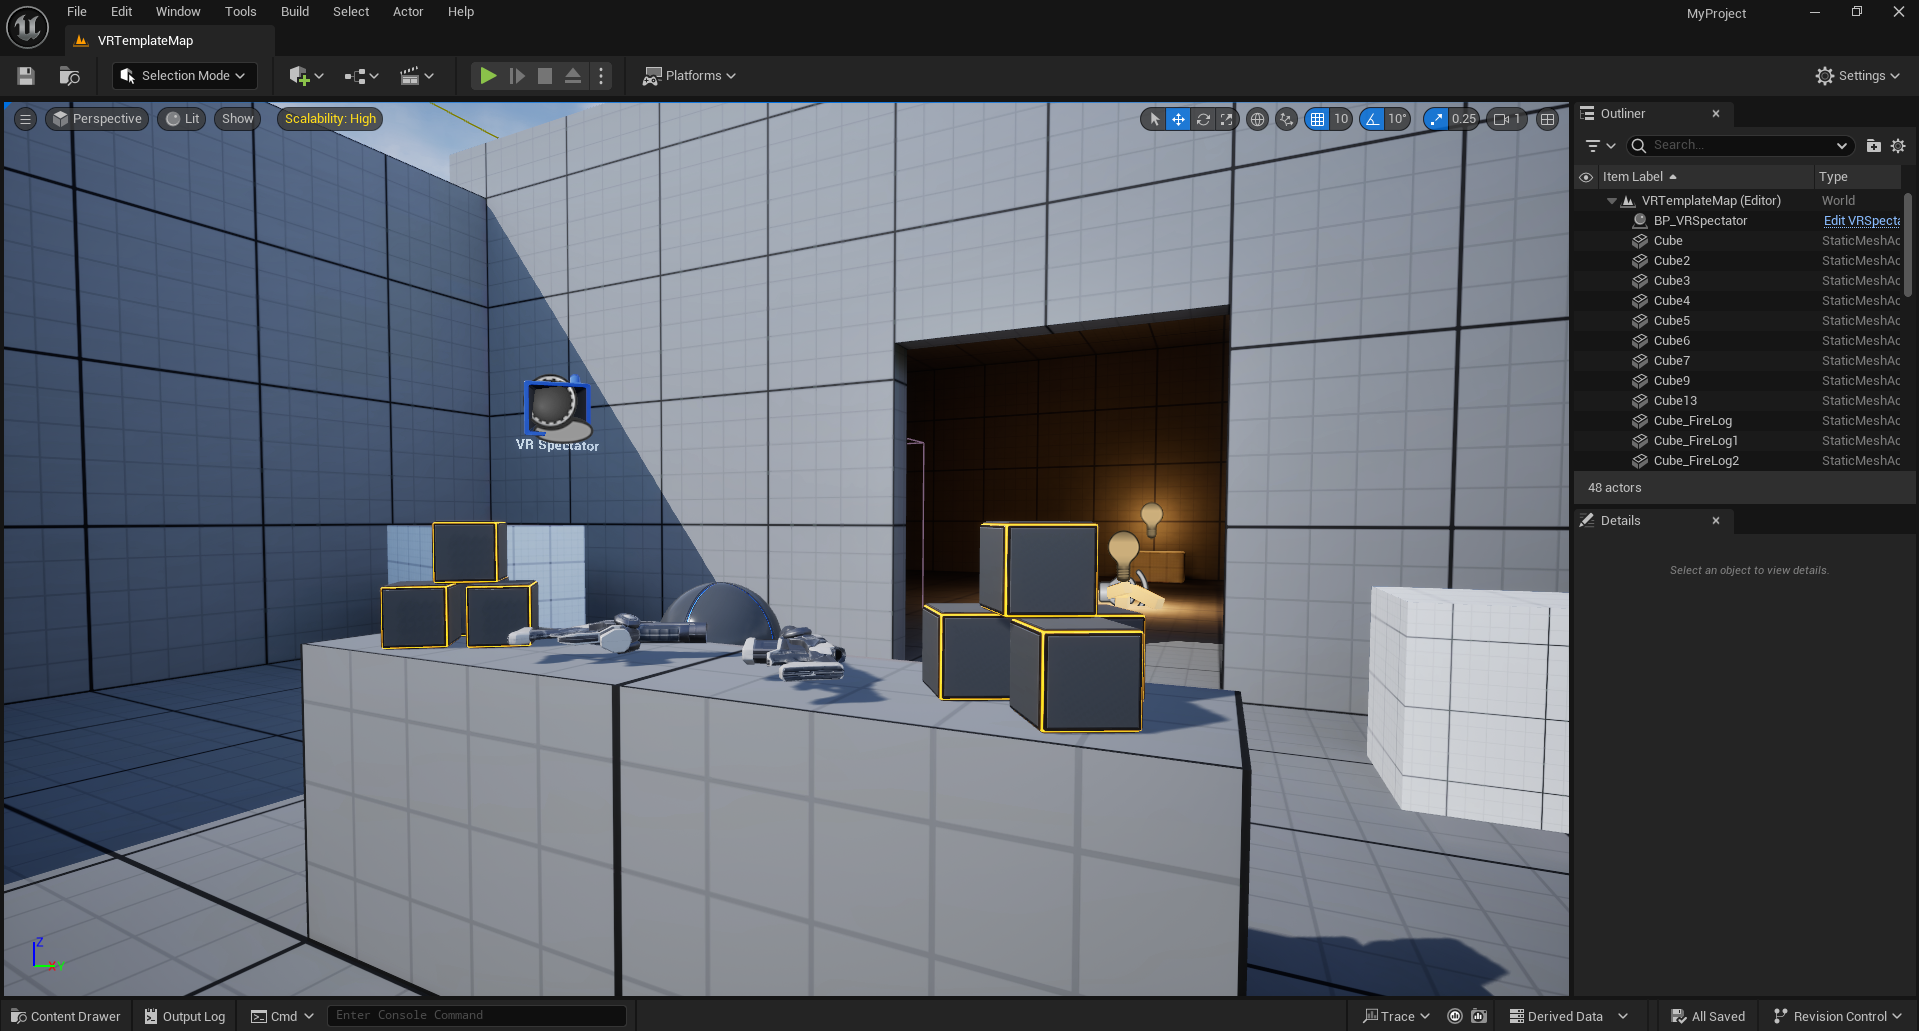
\includegraphics[width=\linewidth, height=6cm]{continut/capitol3/figuri/VR_front.png}
        \label{fig:VR Template}
    \end{subfigure}
    \hfill
    \begin{subfigure}{0.49\textwidth}
        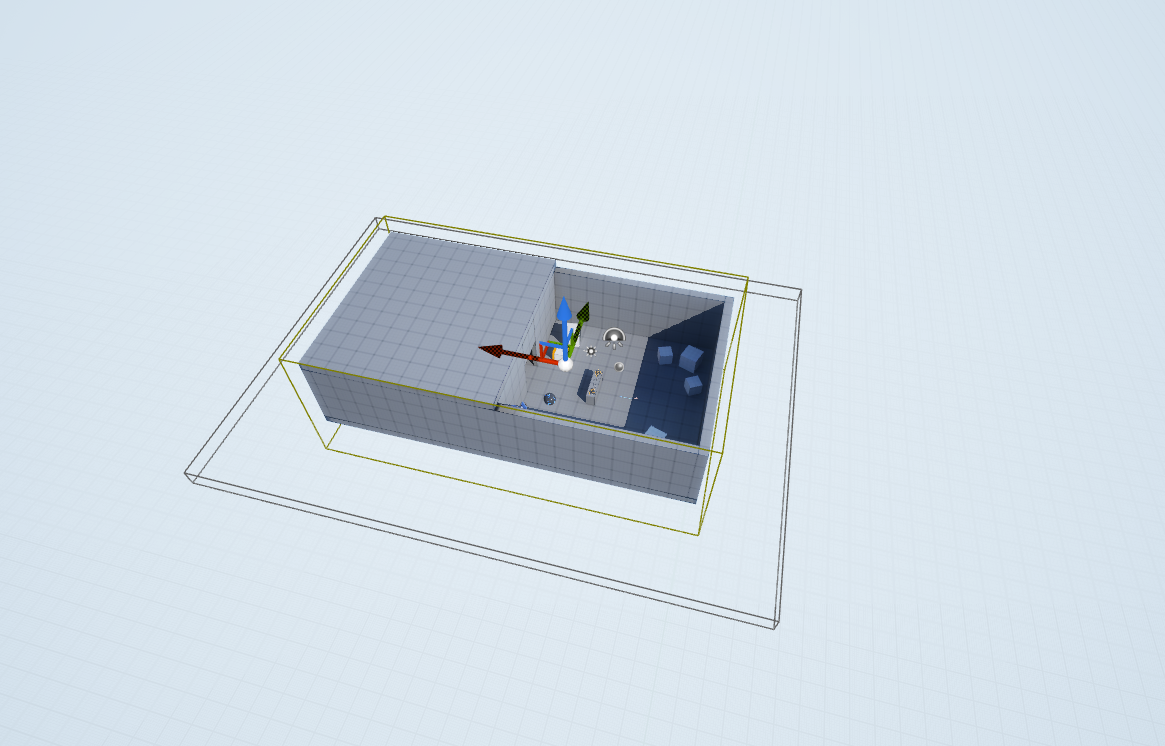
\includegraphics[width=\linewidth, height=6cm]{continut/capitol3/figuri/VR_up.png}
        \label{fig:VR Template}
    \end{subfigure}

    \caption{VR Template}
\end{figure}

Proiectul generat pe baza acestui șablon include o scenă simplă, structurată în două zone: una interioară, asemănătoare unei camere, și una exterioară, expusă la cer. În interiorul scenei se regăsesc mai multe obiecte 3D, unele dintre acestea fiind interactive - pot fi apucate (grab) și manipulate cu ajutorul controlerelor VR. Interacțiunea se realizează natural, prin folosirea butonului de prindere de pe manetă, iar obiectele reacționează în funcție de tipul definit în sistemul de prindere (Snap sau Free Grab).

În zona interioară este prezent un element ambiental format dintr-un foc de tabără. Acesta este compus din câteva cărămizi care simulează reflexii luminoase dinamice și un efect sonor realist ce imită sunetul lemnelor care ard. Aceste elemente contribuie la crearea unei atmosfere imersive și ajută la testarea performanței aplicației în condiții diverse de lumină și sunet.

Locomoția în această experiență se realizează printr-o metodă standard de deplasare în VR, numită teleportare. Utilizatorul poate activa acest sistem prin joystick-ul de pe maneta stângă. În momentul acționării, din mâna stângă este proiectată o linie vizuală ce indică direcția și destinația dorită. După selectarea poziției, teleportarea are loc în momentul eliberării joystick-ului. Sistemul este configurabil, putând fi ajustate zona de destinație, raza de teleportare sau feedback-ul vizual.

Pe lângă deplasare, șablonul integrează și un sistem de rotație incrementală, acționat prin joystick-ul de pe maneta dreaptă. Acesta permite utilizatorului să rotească avatarul la stânga sau la dreapta în pași predefiniți (snap turn), contribuind la reducerea disconfortului asociat cu rotația continuă în VR. Viteza și unghiul fiecărei rotații pot fi configurate în editorul Blueprint.

Template-ul include și un sistem de meniuri interactive în realitate virtuală, activate prin apăsarea unui buton dedicat de pe controler. Acestea sunt afișate sub forma unor ferestre 3D, care pot fi poziționate în fața utilizatorului și utilizate pentru setări, navigare sau informații suplimentare.

Din punct de vedere tehnic, proiectul conține mai multe Blueprint-uri predefinite, fiecare responsabil pentru funcționalitățile principale: deplasarea prin teleport, rotația incrementală, sistemul de prindere a obiectelor și gestionarea meniurilor. Acestea sunt ușor de înțeles și de personalizat, fiind bine documentate atât în interiorul editorului, cât și prin surse externe.

Alegerea acestui template a avut un impact semnificativ în simplificarea procesului de dezvoltare. Deși toate funcționalitățile prezentate puteau fi construite manual de la zero, utilizarea unui cadru existent a permis focalizarea pe aspectele creative și educaționale ale proiectului. În plus, VR Template beneficiază de o comunitate activă și o bază solidă de documentație oficială oferită de Epic Games, ceea ce a facilitat învățarea și adaptarea rapidă în cadrul proiectului VR Museum.

\section{Cadrul virtual}

În cadrul experienței virtuale VR Museum, utilizatorul are posibilitatea de a explora un muzeu de istorie naturală într-un mediu imersiv, conceput pentru a oferi atât elemente educaționale, cât și momente de descoperire interactivă. Totuși, forma actuală a proiectului nu a fost prezentă de la început; inițial, direcția aleasă a fost una mai ambițioasă și complexă, dar dificil de realizat în condițiile tehnice disponibile.

\begin{figure}[h!]
    \centering
    \begin{subfigure}{0.49\textwidth}
        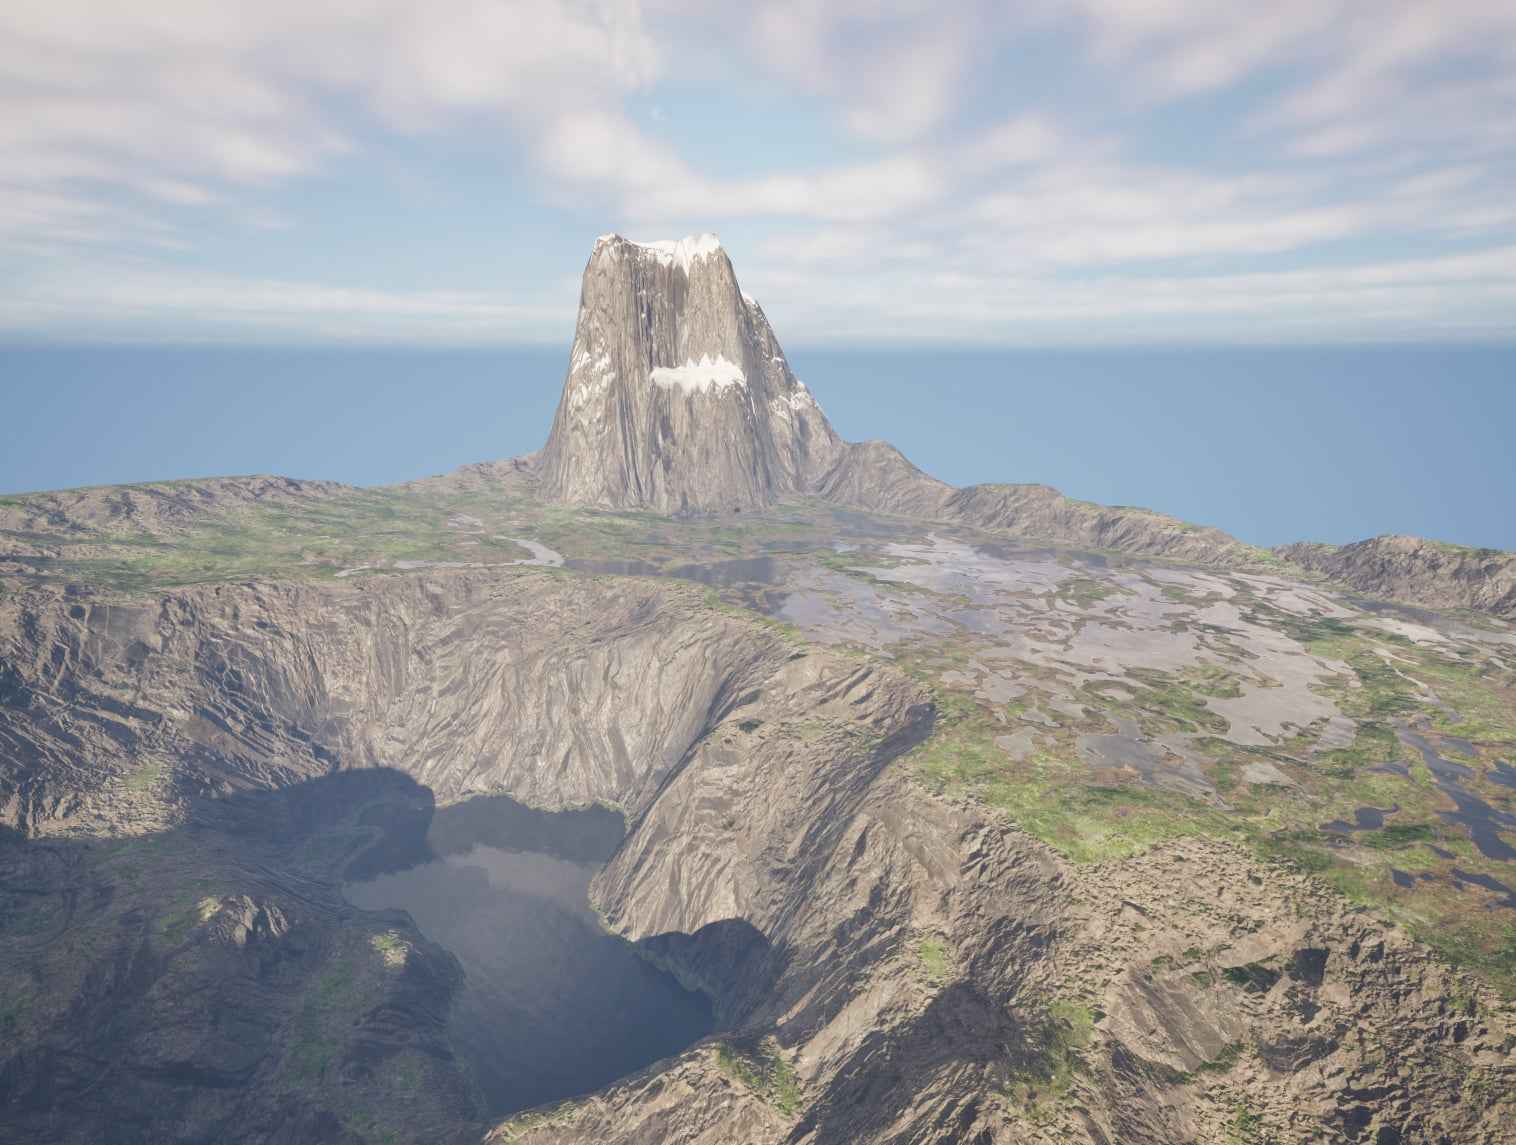
\includegraphics[width=\linewidth, height=6cm]{continut/capitol3/figuri/attempt.jpg}
        \label{fig:First VR attempt}
    \end{subfigure}
    \hfill
    \begin{subfigure}{0.49\textwidth}
        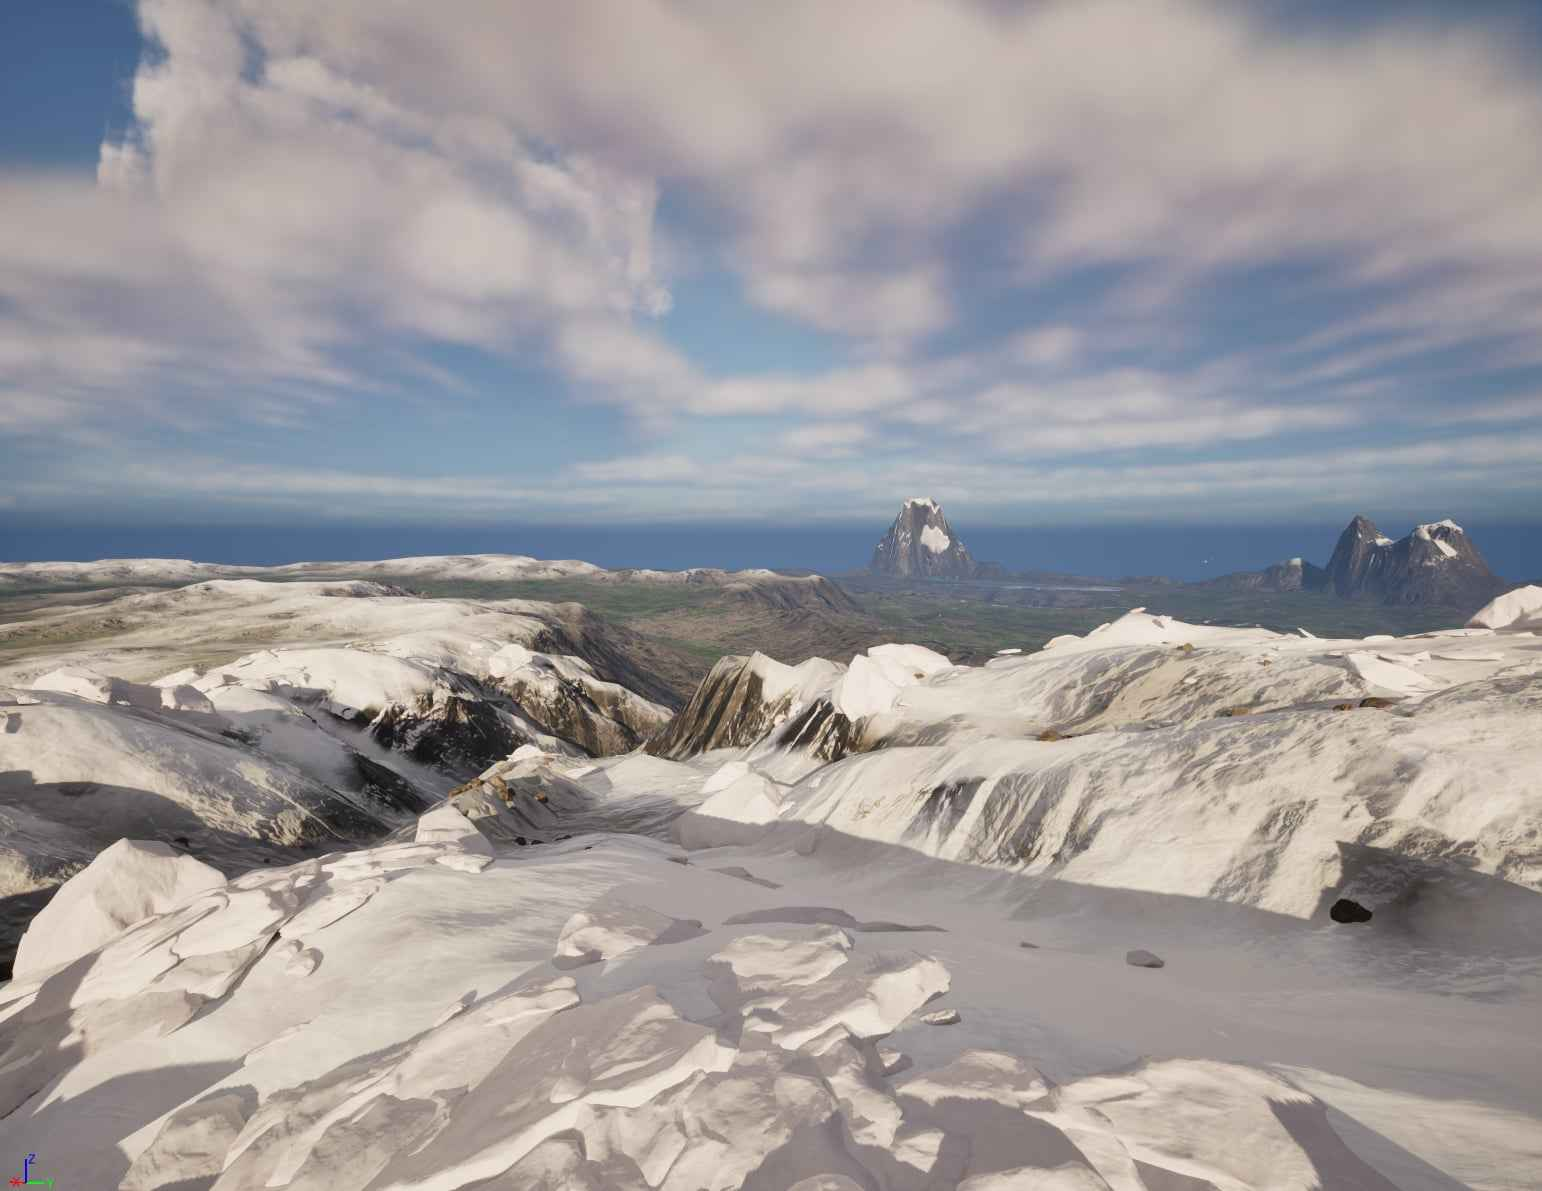
\includegraphics[width=\linewidth, height=6cm]{continut/capitol3/figuri/attempt1jpg.jpg}
        \label{fig:First VR attempt}
    \end{subfigure}

    \caption{Proiecutl initial}
\end{figure}

Versiunea inițială a proiectului includea un spațiu extins, compus dintr-o încăpere de pornire de dimensiuni reduse, care acționa ca un punct de introducere, urmat de o zonă largă, asemănătoare unei poieni deschise, unde utilizatorul putea explora mai multe expoziții dedicate dinozaurilor. Peisajul era vast și detaliat, oferind impresia unui mediu natural neîngrădit, departe de civilizația cotidiană. Deși zonele periferice ale scenei nu erau accesibile direct, designul acestora contribuia la senzația de profunzime și izolare - un spațiu fictiv, dar credibil, menit să stimuleze curiozitatea și să creeze atmosfera unei călătorii în timp.

Fiecare expoziție era dedicată unei specii de dinozaur, prezentând o combinație între modelul tridimensional al animalului și informații descriptive. Panourile interactive amplasate în jurul exponatului ofereau detalii despre perioada în care trăia specia respectivă, obiceiuri alimentare, habitat și descoperiri științifice relevante. Printre aceste panouri se regăsea și un buton intitulat „Preview”, a cărui funcție era să teleporteze utilizatorul într-un mediu special recreat pentru acea epocă istorică. Aceste scene tematice simulau condițiile de mediu - vegetație preistorică, climă, iluminare specifică și chiar sunete ambientale precum ciripitul reptilelor primitive sau foșnetul frunzelor mari - totul gândit pentru a oferi o experiență completă și educativă.

În anumite cazuri, scena „preview” includea și o formă limitată de interacțiune: utilizatorul putea observa dinozaurul în mișcare, putea urmări o simulare de comportament specific (de exemplu, hrănire sau apărare), iar unele elemente ale mediului răspundeau la acțiunile acestuia (de exemplu, vegetația se mișca la apropiere). Această abordare avea scopul de a oferi nu doar o experiență pasivă de vizionare, ci una activă, bazată pe explorare și imersiune contextuală.

Astfel, s-a optat pentru o variantă mai realistă și fezabilă: un muzeu structurat în principal ca un spațiu interior, dar care include și o componentă exterioară. Această alegere a permis organizarea expozițiilor într-un mod mai coerent și ușor de gestionat, fără a compromite scopul educativ sau caracterul interactiv al experienței. De asemenea, am putut investi mai mult timp în perfecționarea accesibilității - prin optimizarea controalelor, a interfeței și a performanței aplicației - și în atragerea unui public mai larg, inclusiv utilizatori care nu sunt familiarizați cu tehnologia VR.

Prin această tranziție de la o idee conceptuală ambițioasă către o execuție practică și focalizată, proiectul VR Museum a reușit să păstreze esența scopului său - educarea prin explorare imersivă - fără a compromite stabilitatea, claritatea și calitatea experienței finale.

Pentru implementarea proiectul, s-a construit cladirea in care vor fi adaugate restul de obiecte, expozitii, etc.

\section{Alcatuirea muzeului și a spațiului înconjurător}

\begin{figure} [htp] 
\centering 
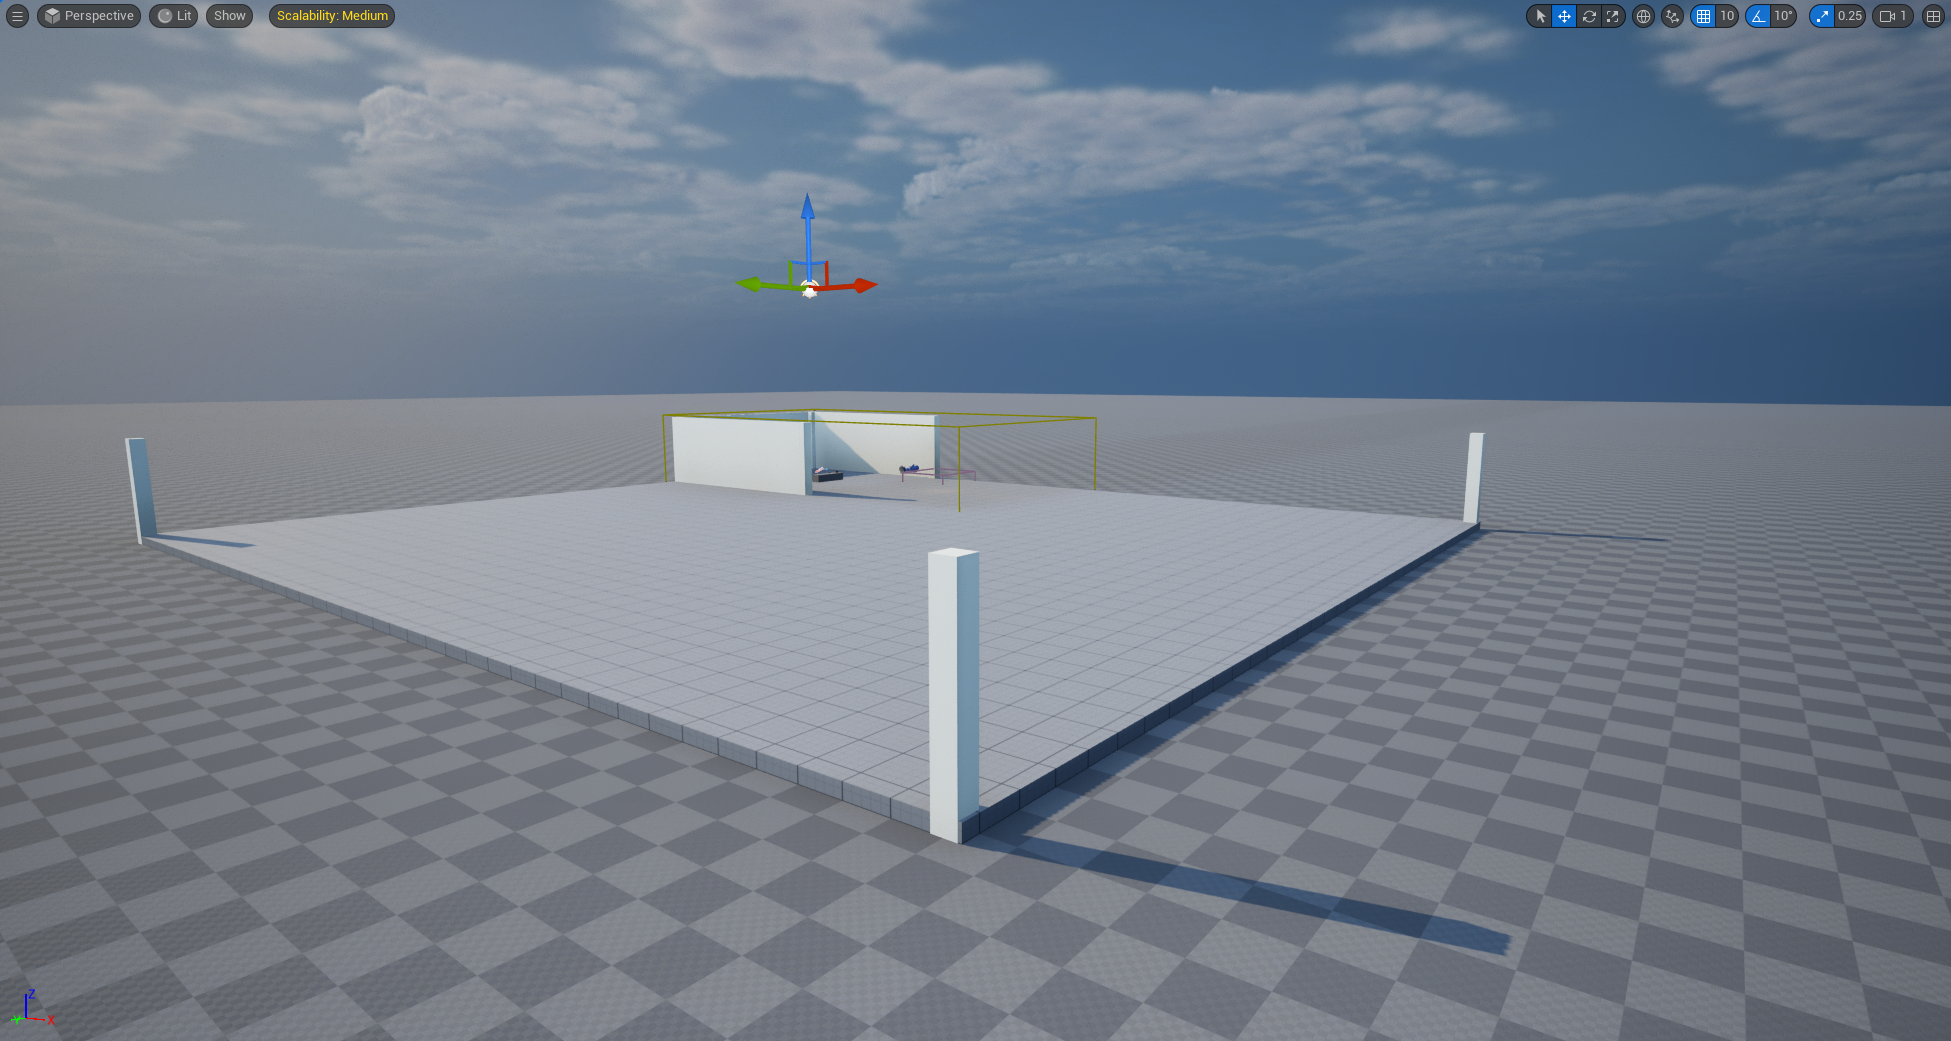
\includegraphics [width=12cm]
{continut/capitol3/figuri/beginning.png} 
\caption{Alcătuirea muzeului} 
\label{fig:Museum} 
\end{figure}

Arhitectura muzeului a fost construită utilizând obiectele disponibile în pachetul StarterContent, oferit gratuit odată cu șablonul Unreal Engine. Aceste elemente de bază au constituit punctul de plecare pentru amenajarea spațiului interior, fiind alese pentru simplitatea integrării și compatibilitatea directă cu structura proiectului.
\begin{figure}[h!]
    \centering
    \begin{subfigure}{0.49\textwidth}
        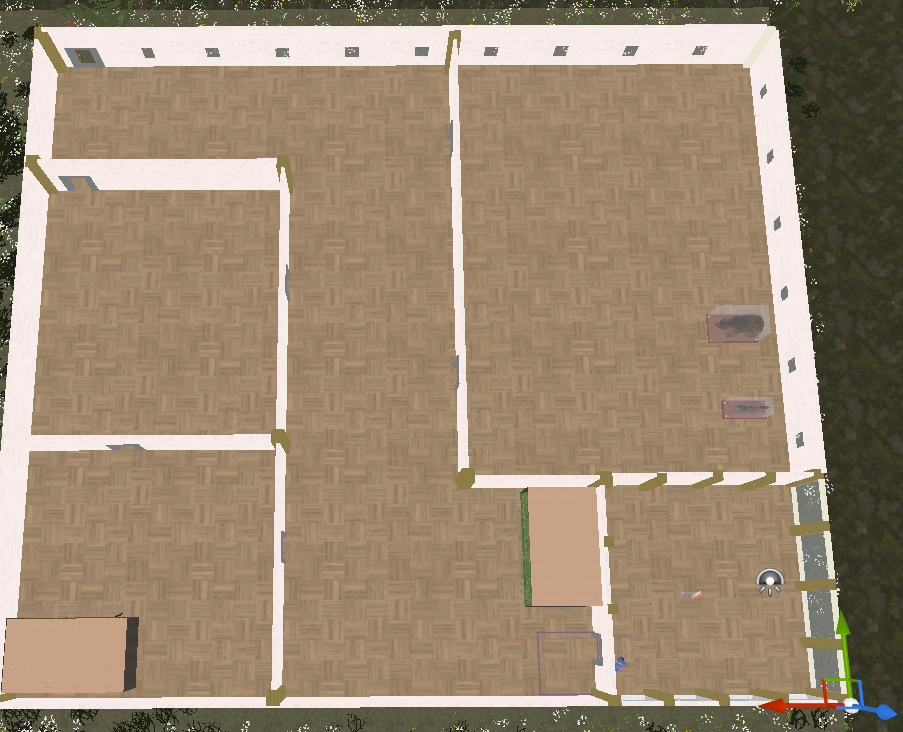
\includegraphics[width=\linewidth, height=6cm]{continut/capitol3/figuri/scheme.png}
        \label{fig:Museum}
    \end{subfigure}
    \hfill
    \begin{subfigure}{0.49\textwidth}
        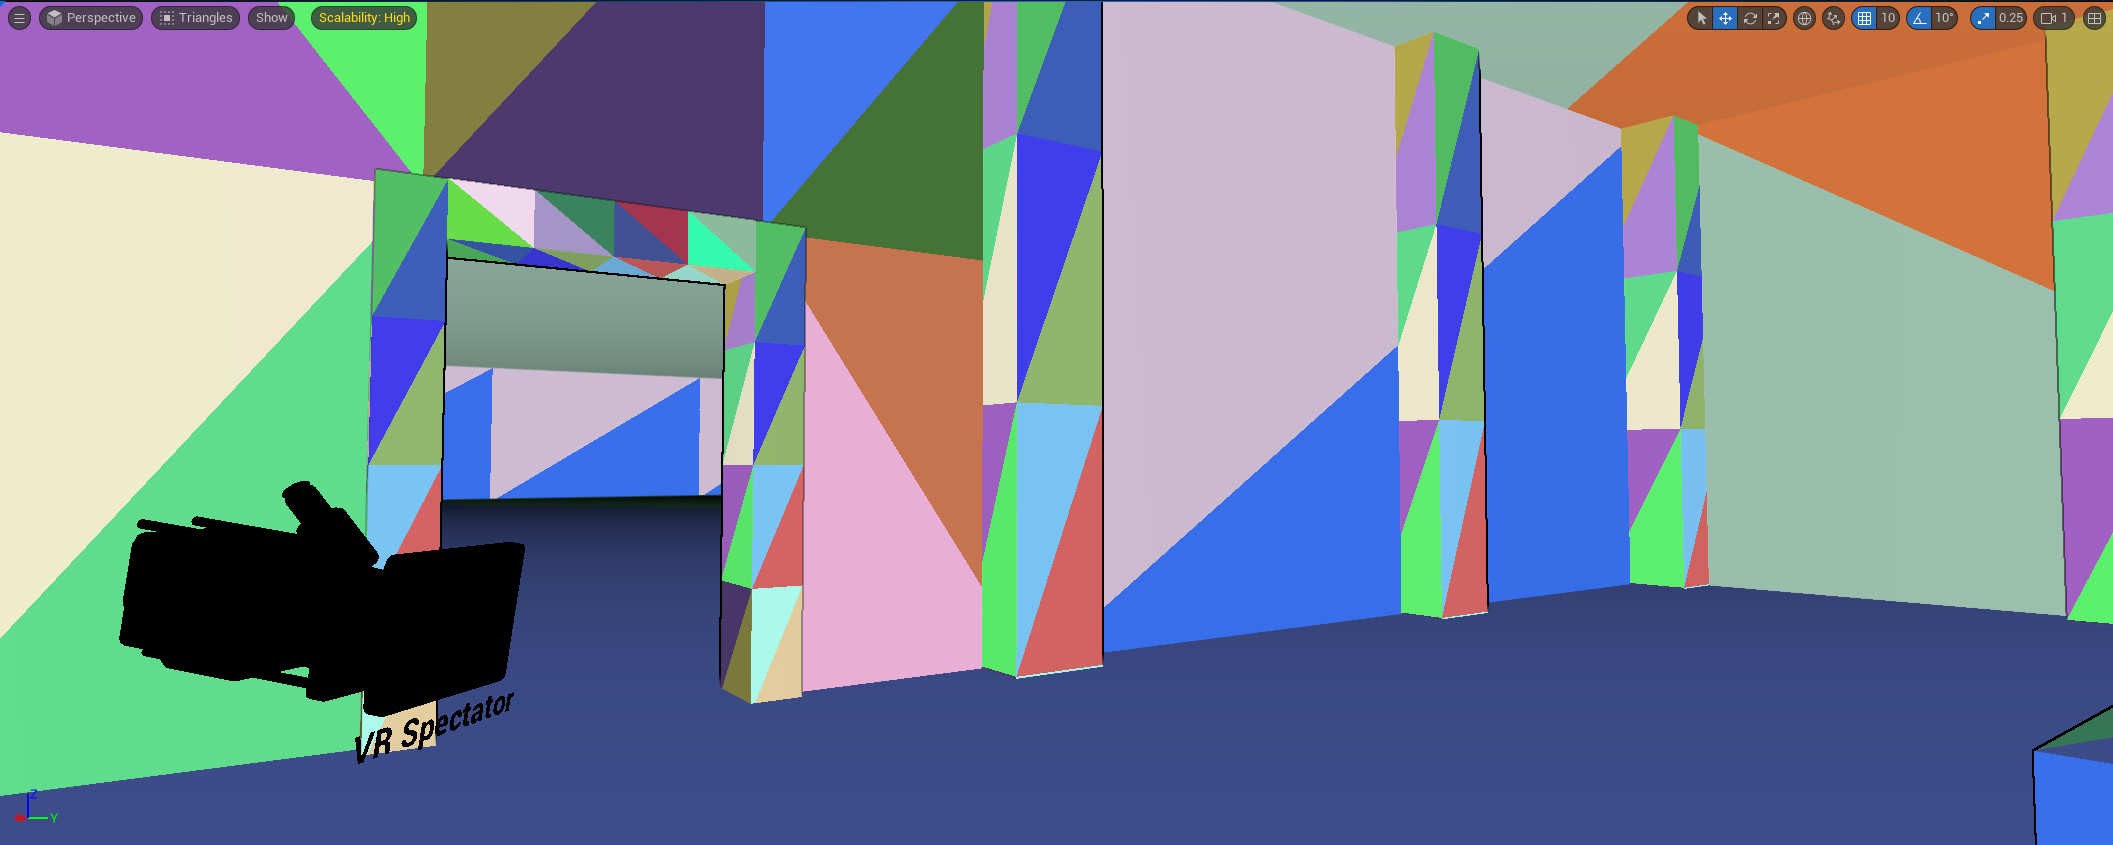
\includegraphics[width=\linewidth, height=6cm]{continut/capitol3/figuri/Screenshot 2025-03-03 135626.png}
        \label{fig:Museum}
    \end{subfigure}
    \caption{Alcătuirea mzeului - camera si utilizarea tehnologii Nanite pentru modelarea obiectelor}
\end{figure}

\begin{figure}[h!]
    \centering
    \begin{subfigure}{0.49\textwidth}
        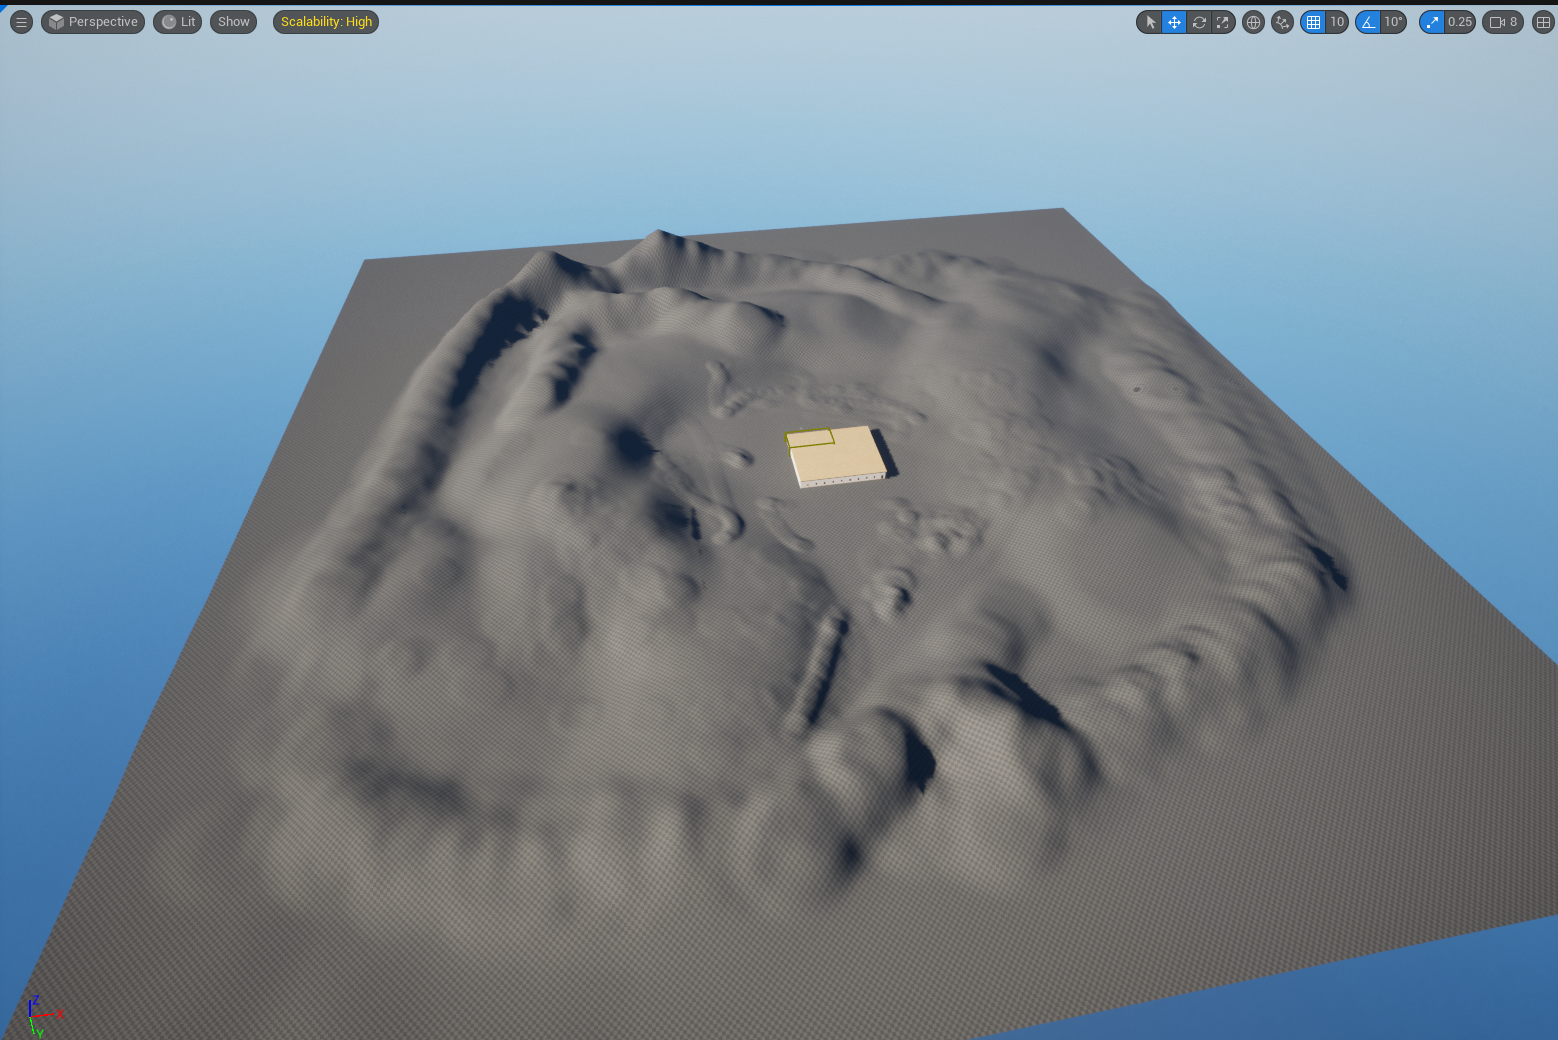
\includegraphics[width=\linewidth, height=6cm]{continut/capitol3/figuri/3_terrain_mapping.png}
        \label{fig:Terrain mapping}
    \end{subfigure}
    \hfill
    \begin{subfigure}{0.49\textwidth}
        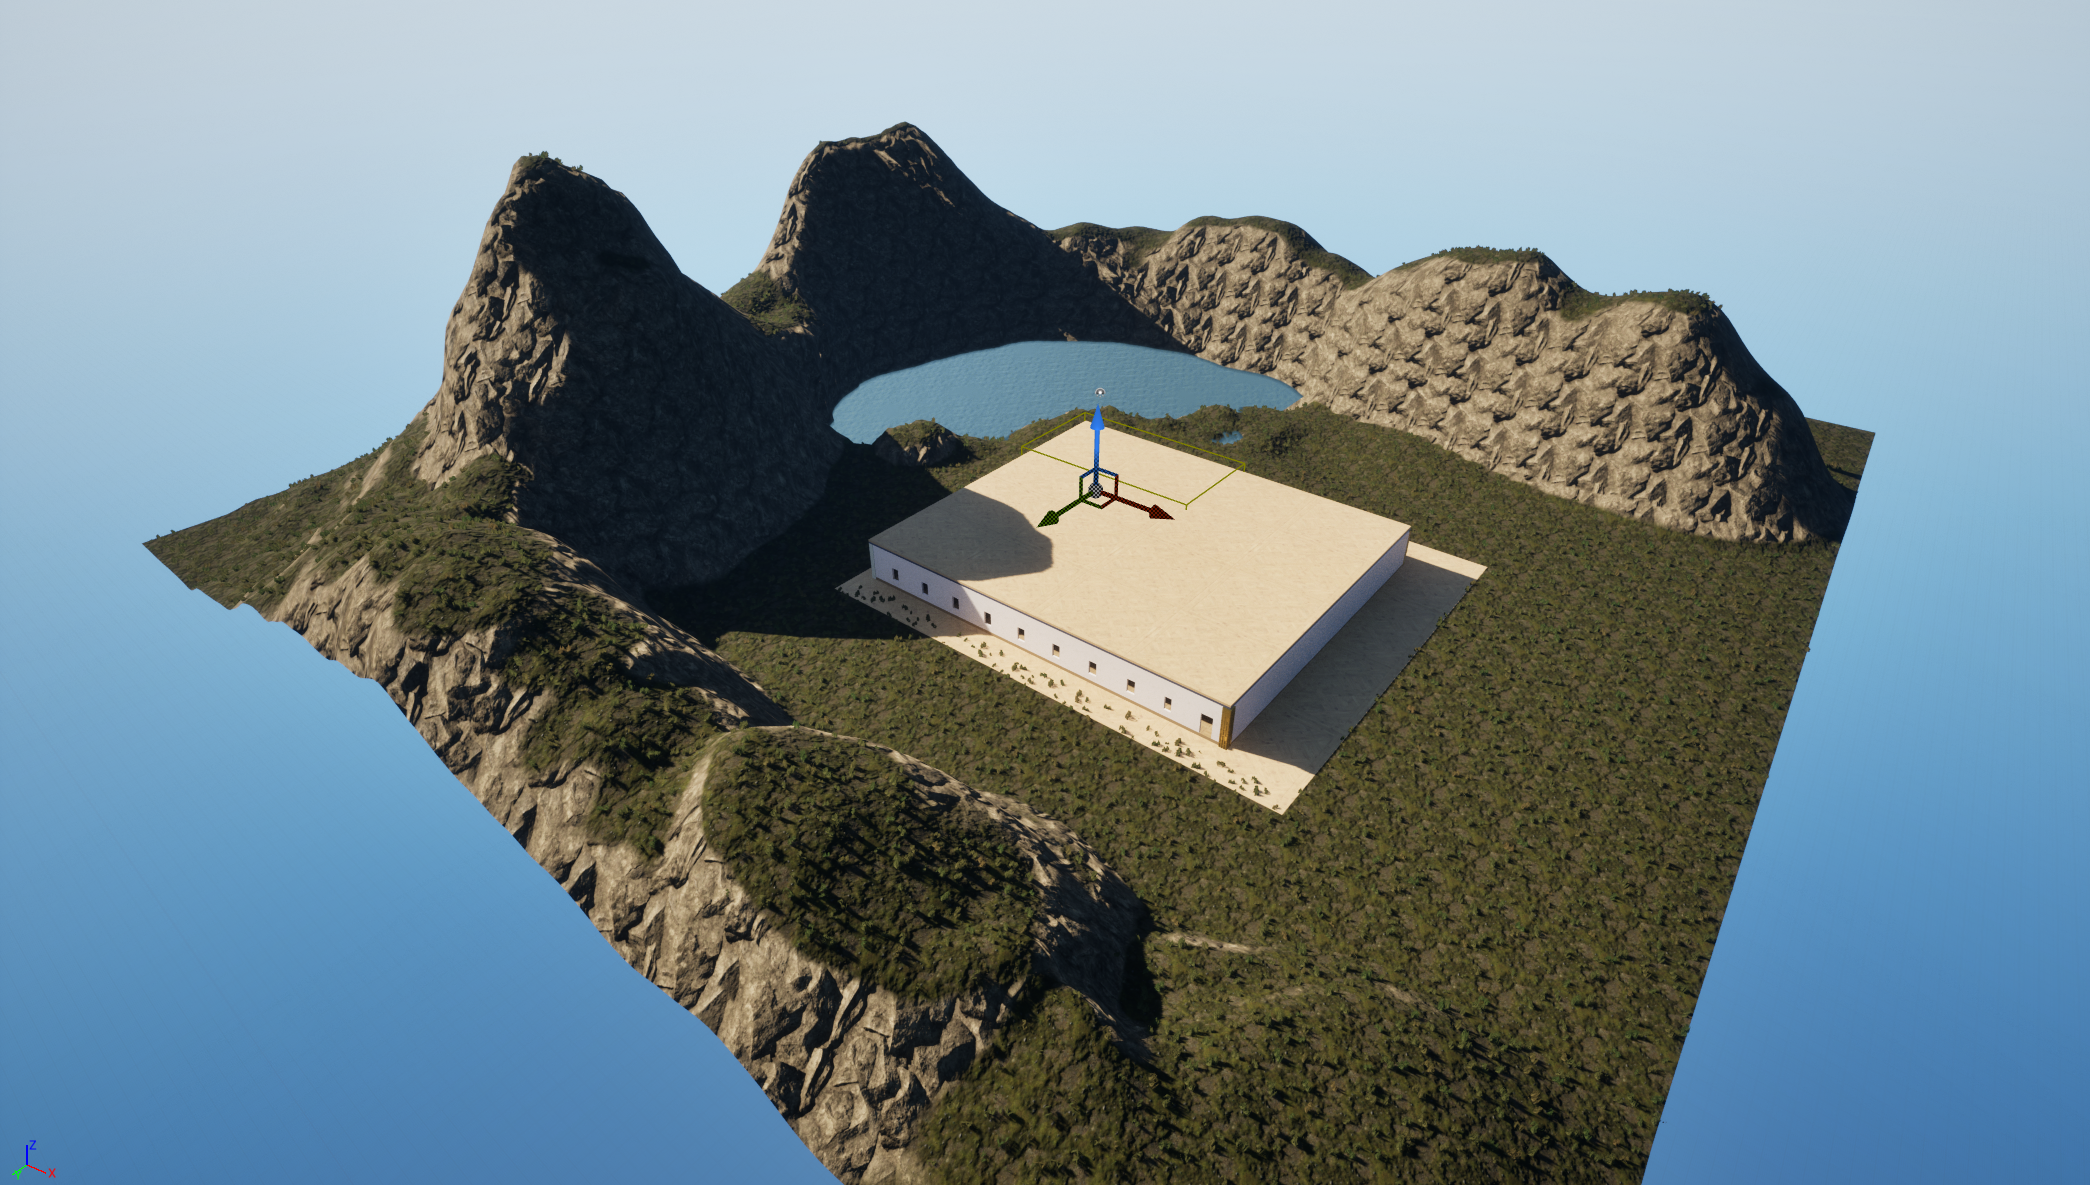
\includegraphics[width=\linewidth, height=6cm]{continut/capitol3/figuri/4_terrain_texture.png}
        \label{fig:Terrain mapping}
    \end{subfigure}
    \begin{subfigure}{0.49\textwidth}
        \includegraphics[width=\linewidth, height=6cm]{continut/capitol3/figuri/5_terrain_props.png}
        \label{fig:Terrain mapping}
    \end{subfigure}
    \begin{subfigure}{0.49\textwidth}
        \includegraphics[width=\linewidth, height=6cm]{continut/capitol3/figuri/6_state.png}
        \label{fig:Terrain mapping}
    \end{subfigure}

    \caption{Alcătuirea terenului}
\end{figure}
Procesul de organizare a spațiului a fost unul provocator. Deși ideile de design erau numeroase, găsirea unei soluții coerente și echilibrate din punct de vedere vizual a necesitat mai multe iterații. Inițial, muzeul a fost conceput ca un spațiu mare, deschis, fără compartimentări clare, cu scopul de a oferi flexibilitate în faza de construcție. Ulterior, acest spațiu a fost adaptat și segmentat în zone distincte, în funcție de tematica expozițiilor și de traseul pe care utilizatorul îl poate urma.

După stabilirea structurii interioare, atenția a fost direcționată către mediul exterior - peisajul virtual. Crearea acestuia a reprezentat o etapă interesantă și esențială pentru coerența vizuală a proiectului. Terenul a fost modelat manual prin instrumentele de Landscape Sculpting, adăugând munți, zone depresionare, potențiale cursuri de apă și mici denivelări care să simuleze un relief realist. Scopul a fost acela de a reda un cadru cât mai apropiat de natură, cu variații subtile de altitudine și volum care să elimine senzația de artificial sau plat. Jocul de lumină pe aceste suprafețe neregulate, împreună cu materialele de sol aplicate, contribuie la crearea unei atmosfere care, pe alocuri, poate părea apropiată de realitate.

Pentru a limita zona de explorare și a păstra imersiunea, au fost adăugate margini invizibile la extremitățile hărții. Aceste bariere împiedică utilizatorul să părăsească zona activă sau să observe capătul scenei, evitând astfel senzația că spațiul virtual este „tăiat” brusc ori incomplet.

Decorarea spațiului muzeal, precum și a zonei exterioare, a implicat integrarea unei game variate de materiale și obiecte decorative. Acestea au fost atent alese pentru a crea o experiență vizuală plăcută, diversificată și convingătoare din punct de vedere estetic.

\section{Materialele in Unreal Engine}

Pentru a adăuga detalii vizuale obiectelor din cadrul experienței VR, este necesară aplicarea unor materiale. În Unreal Engine, un material reprezintă un set complex de proprietăți vizuale care determină modul în care un obiect va reflecta lumina, ce culoare va avea, cât de rugos sau lucios va părea și ce detalii de suprafață va reda.

\begin{figure}[h!]
    \centering
    \begin{subfigure}{0.49\textwidth}
        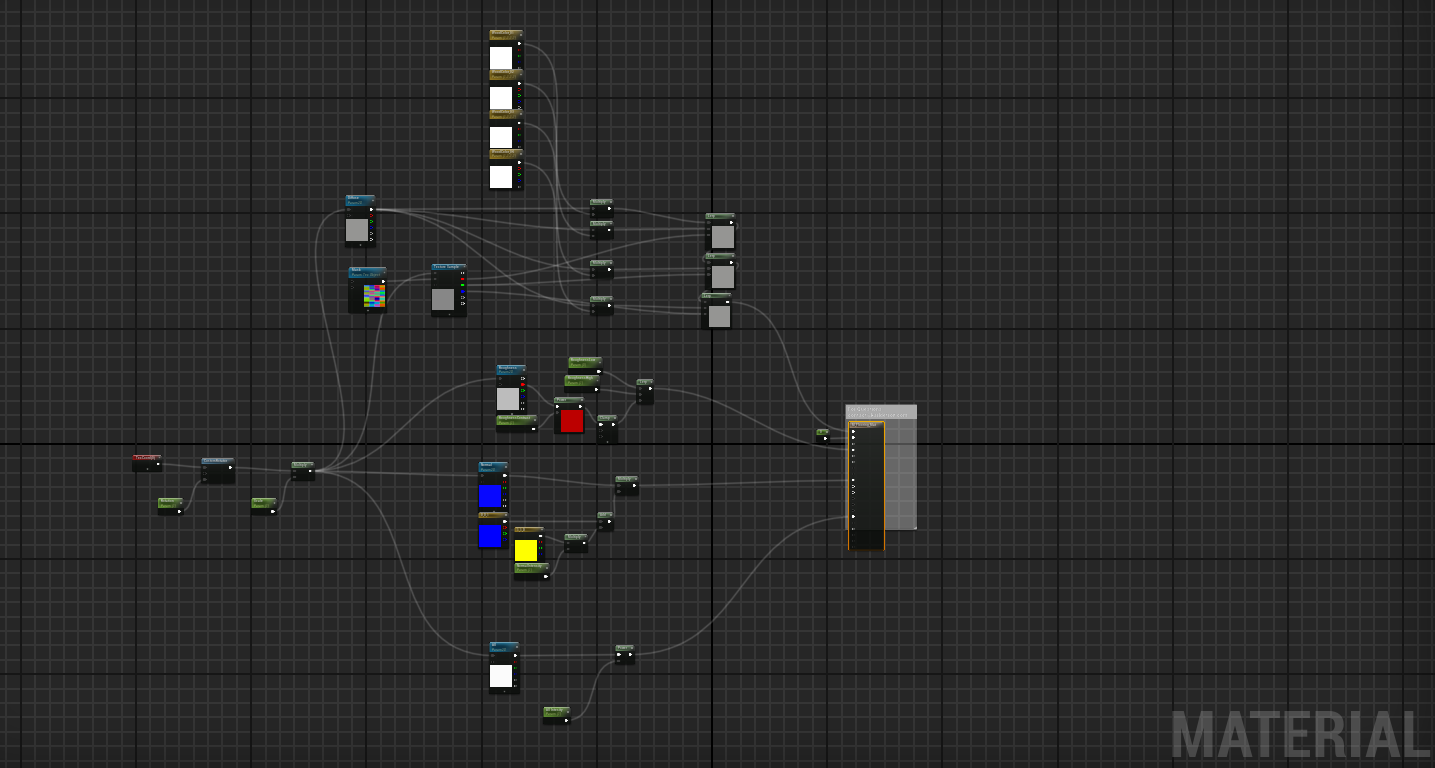
\includegraphics[width=\linewidth, height=6cm]{continut/capitol3/figuri/material.png}
        \label{fig:Terrain mapping}
    \end{subfigure}
    \hfill
    \begin{subfigure}{0.49\textwidth}
        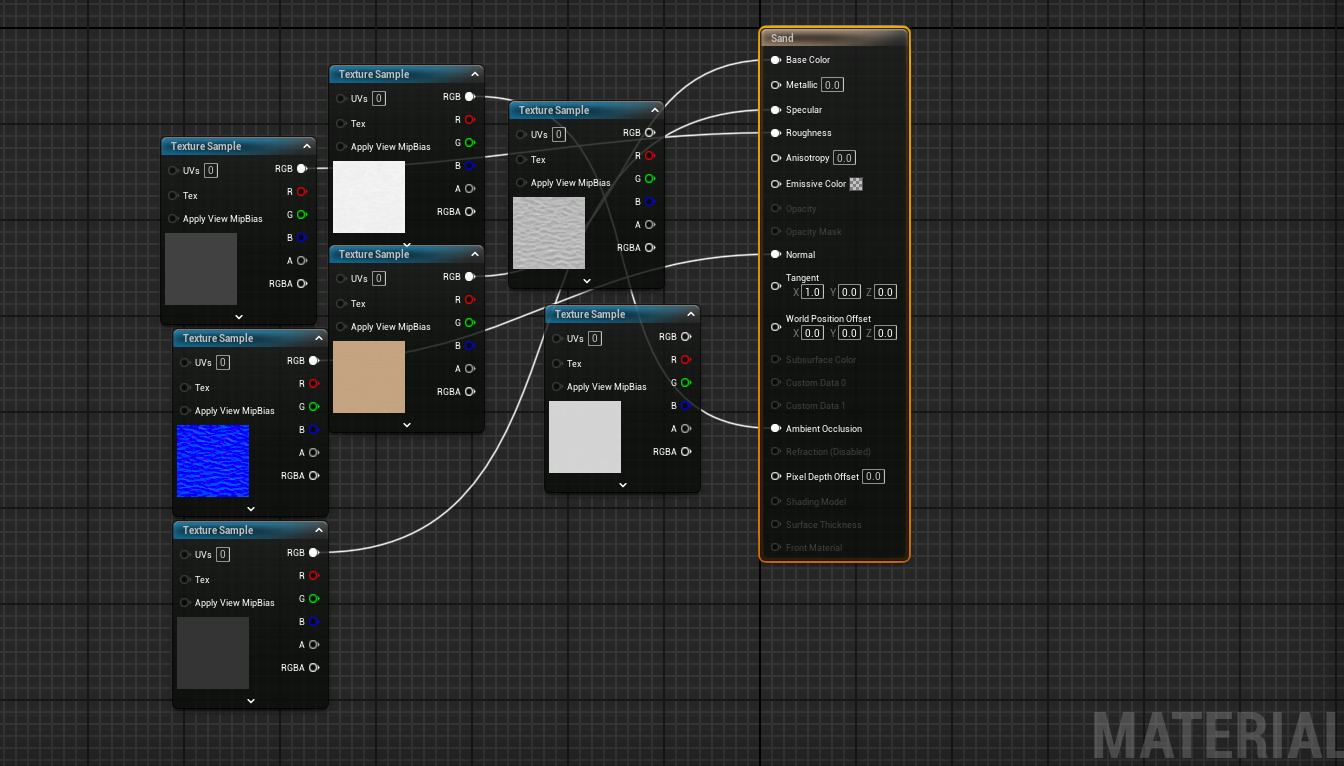
\includegraphics[width=\linewidth, height=6cm]{continut/capitol3/figuri/ez_mat.png}
        \label{fig:Terrain mapping}
    \end{subfigure}
    \caption{Un material din VR Museum}
\end{figure}

Materialele nu sunt doar culori simple aplicate pe obiecte, ci sunt compuse din mai multe texturi, fiecare având un rol specific. Aceste texturi sunt combinate într-un grafic de tip Material Editor, care permite conectarea și controlul parametrilor pentru a genera un rezultat final realist sau stilizat, în funcție de nevoile proiectului. În cele ce urmează sunt prezentate cele mai utilizate tipuri de texturi în crearea unui material de bază:

\begin{itemize}
\item \textbf{Base Color (Albedo)} - definește culoarea de bază a materialului, fără umbre sau influențe de iluminare. Este, practic, componenta vizuală dominantă care determină cum „arată” suprafața în condiții de lumină neutră. Nu conține informații despre reflexii, luciu sau profunzime, ci doar cromatică pură.
\item \textbf{Normal Map} - o textură care simulează detalii fine de suprafață, cum ar fi zgârieturi, crăpături sau muchii, fără a modifica geometria reală a obiectului. Aceasta afectează modul în care lumina interacționează cu suprafața, oferind iluzia de volum și complexitate. Este extrem de utilă în optimizarea performanței, deoarece creează detalii vizuale fără a adăuga poligoane suplimentare.
\item \textbf{Metallic} - efinește cât de metalică este suprafața materialului. Valorile ridicate (apropiate de 1) indică un material care reflectă lumina în mod specific unui metal (de exemplu, fier, aluminiu), în timp ce valorile apropiate de 0 indică un material nemetalic, cum ar fi piatra, lemnul sau plasticul. De obicei, această textură este în tonuri de gri sau alb-negru.
\item \textbf{Roughness} - controlează cât de netedă sau rugoasă este suprafața. O valoare mică (spre 0) indică o suprafață foarte lucioasă, cum ar fi sticla sau metalul lustruit, în timp ce o valoare mare (spre 1) descrie o suprafață mată și difuză, cum ar fi cimentul sau hârtia. Acest parametru influențează modul în care sunt vizibile reflexiile.
\item \textbf{Ambient Occlusion (AO)} - opțională, dar foarte utilă pentru adăugarea de umbriri fine în colțuri, margini sau zone în care lumina ambientală ar fi parțial blocată. Aceasta adaugă profunzime și realism suplimentar scenei, mai ales în combinație cu iluminarea globală.
\end{itemize}

Aceste texturi pot fi fie importate din pachete externe, fie generate procedural în editor, și sunt combinate prin noduri logice în editorul de materiale din Unreal Engine. Rezultatul final este un material care poate fi aplicat oricărui obiect 3D din scenă, contribuind esențial la aspectul general al aplicației.

În cadrul proiectului VR Museum, au fost create materiale personalizate atât pentru interiorul muzeului (parchet, pereți, vitrine), cât și pentru mediul exterior (pământ, piatră, vegetație). Fiecare material a fost adaptat pentru a reda o atmosferă coerentă și naturală, urmând principiile de bază ale physically based rendering (PBR).

Pentru crearea terenului din cadrul scenei exterioare, a fost utilizat un asset specializat, numit Landscape Pro. Acesta este un material complex, multifuncțional, care combină în mod procedural mai multe tipuri de suprafețe - pământ, iarbă și rocă - într-un singur shader aplicabil pe sistemul de landscape din Unreal Engine. Avantajul major al acestui asset constă în faptul că, odată aplicat, materialul este capabil să detecteze automat înclinația și forma reliefului și să genereze în mod procedural prop-uri decorative: fire de iarbă, ramuri uscate, frunze căzute, flori, pietre și alte elemente naturale.

Această generare procedurală nu doar că accelerează procesul de construire a unei scene realiste, dar și adaugă un nivel ridicat de detaliu și varietate, greu de obținut manual. Astfel, utilizatorul are senzația că se află într-un mediu natural credibil, viu și dinamic. Fiecare zonă a terenului este compusă dintr-o combinație vizuală de textură de sol și obiecte tridimensionale ușor diferite, ceea ce previne repetitivitatea și accentuează realismul.

Totuși, această complexitate vine cu un cost de performanță semnificativ. Landscape Pro este un material pretențios din punct de vedere al resurselor hardware, în special atunci când se folosesc setările grafice la un nivel ridicat. Obiectele generate procedural - cum ar fi iarbă, frunze sau pietre - adaugă un număr mare de instanțe care trebuie randate în timp real, ceea ce poate afecta negativ fluiditatea experienței VR pe dispozitive mai modeste. Din acest motiv, asset-ul este configurat să reacționeze la setările grafice ale aplicației: atunci când acestea sunt reduse (de exemplu, pentru a obține performanță mai bună pe sisteme cu specificații mai slabe), toate prop-urile adiționale dispar automat, rămânând doar textura de bază aplicată pe teren.

Această tranziție vizuală influențează semnificativ calitatea percepută a mediului înconjurător. La setări maxime, peisajul este bogat, divers și foarte apropiat de un mediu natural real. La setări reduse, scenele rămân funcționale, dar vizibil simplificate. Cu toate acestea, decizia de a utiliza Landscape Pro a fost una justificată de necesitatea unei prezentări vizuale impresionante, în special în contextul explorării unui muzeu în realitate virtuală, unde imersiunea este un factor esențial.

\section{Realizarea asset-urilor}

Asset-urile utilizate într-un proiect Unreal Engine pot proveni din surse variate, fie că sunt special concepute pentru motorul grafic realizat de Epic Games, fie că sunt universale și adaptate ulterior. Indiferent de proveniență, toate asset-urile 3D sunt compuse dintr-o rețea de poligoane - elemente geometrice esențiale care determină forma, complexitatea și nivelul de detaliu al obiectului. Cu cât un asset are mai multe poligoane, cu atât este mai detaliat, dar și mai costisitor din punct de vedere al performanței.

În situația ideală, asset-ul este creat special pentru Unreal Engine și vine deja optimizat, incluzând o structură internă denumită skeleton (schelet). Acest schelet permite animarea obiectului, permițând mișcarea și manipularea părților componente (cum ar fi membrele unui corp sau articulațiile unui robot). În combinație cu un set de animatii - realizate frame cu frame sau generate procedural - acest sistem oferă o bază solidă pentru personaje sau obiecte dinamice care pot reacționa la acțiunile utilizatorului sau la mediul înconjurător.

\begin{figure} [htp] 
\centering 
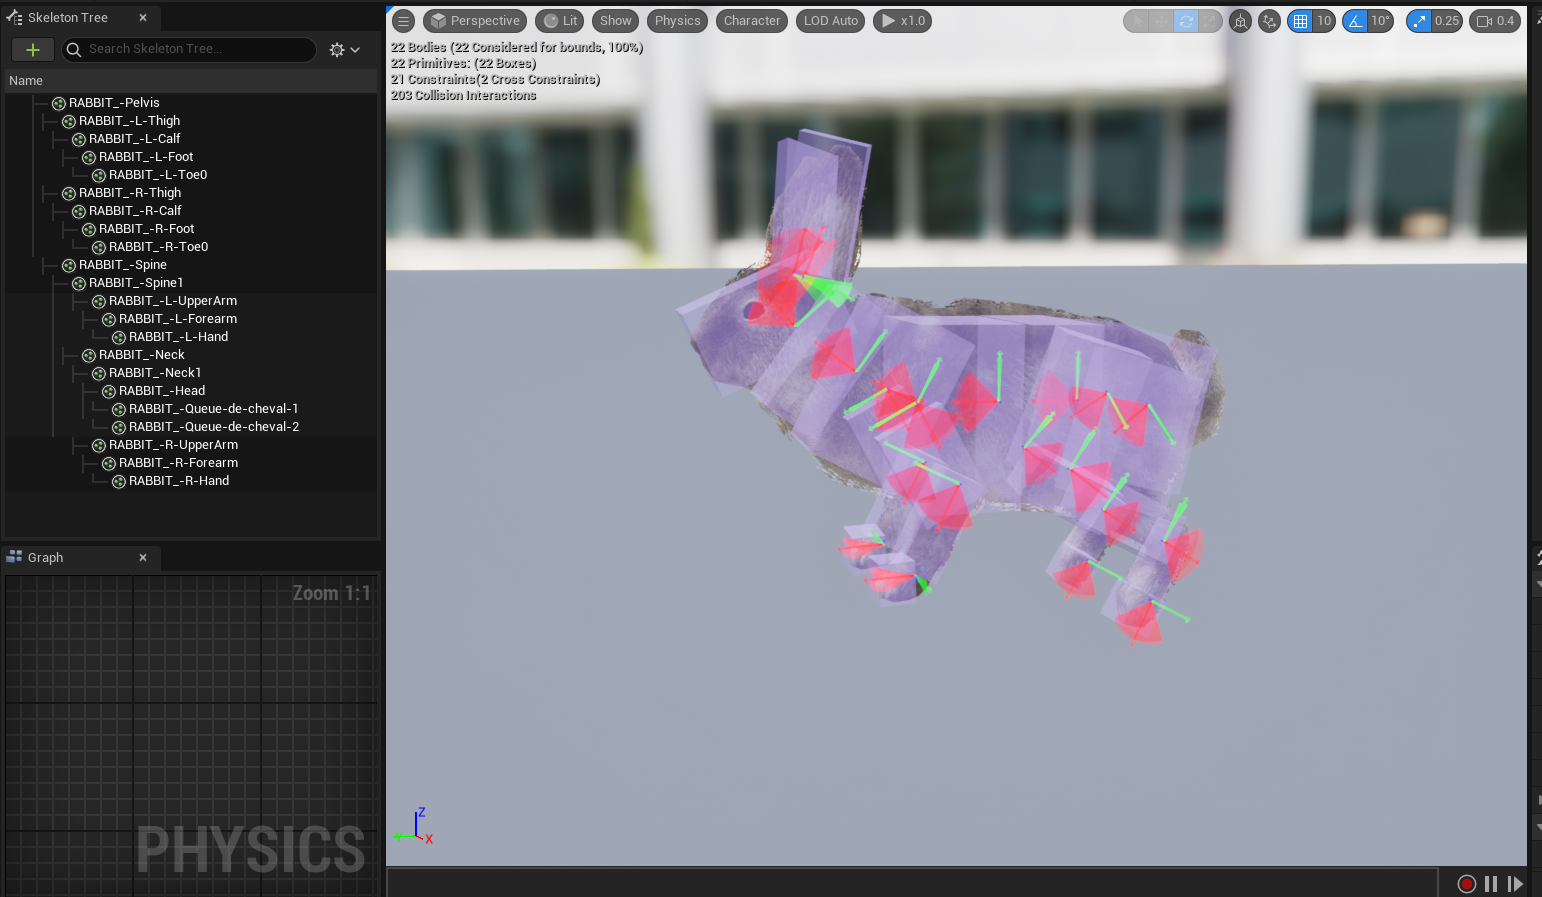
\includegraphics [width=12cm]
{continut/capitol3/figuri/rabbit.png} 
\caption{Animația unui iepure} 
\label{fig:Museum} 
\end{figure}

Pentru animarea acestor asset-uri, se folosește adesea o abordare de tip frame-by-frame, în care pozițiile oaselor și deformările de mesh sunt atent reglate pentru fiecare cadru al secvenței. Acest proces este unul laborios, care necesită precizie și atenție pentru a asigura mișcări fluide și realiste. În cazul proiectului VR Museum, însă, s-a optat pentru o soluție mai simplă: asset-urile animate au fost convertite în Static Meshes, adică obiecte statice, care nu mai pot fi animate, dar pot fi plasate direct în scenă. Această decizie a fost luată pentru a reduce complexitatea proiectului și a evita eventuale probleme de compatibilitate.

Pentru asset-urile care nu au fost concepute special pentru Unreal Engine, integrarea a presupus un proces suplimentar de convertire. Aceste resurse externe au fost descărcate din diverse surse și transformate în formatul glTF (.glb sau .gltf), unul dintre cele mai populare și versatili pentru schimbul de modele 3D. Odată convertite, ele au fost importate în editorul Unreal, însă nu fără dificultăți.

În numeroase cazuri, conversia a provocat probleme majore legate de coliziune, dimensiuni incorecte sau descompunerea asset-ului în componente multiple. Unele modele importate aveau o scară extrem de mică (ex. 0.0005), ceea ce a dus la pierderea completă a coliziunilor sau la comportamente neprevăzute în scenă. Aceste asset-uri au necesitat intervenții manuale: redimensionare, ajustare a ancorelor, eliminarea coliziunilor greșite și gruparea componentelor individuale într-un singur element logic. În unele cazuri, un singur prop era alcătuit din peste 30 de subcomponente, ceea ce a însemnat ore întregi de muncă suplimentară.

Unreal Engine suportă o varietate de formate de fișiere 3D, printre care .fbx, .glb/.gltf, .usdz sau .obj. Totuși, din toate aceste opțiuni, doar formatul glTF s-a dovedit a fi fiabil pentru fluxul de lucru folosit în acest proiect, chiar dacă au existat probleme frecvente legate de scalare și organizare internă. Formatul .fbx, deși foarte popular, a prezentat în unele cazuri erori la import, iar celelalte formate (precum .usdz) nu au oferit controlul necesar asupra parametrilor de compunere.

Integrarea asset-urilor în proiectul VR Museum a reprezentat una dintre cele mai laborioase etape ale procesului de dezvoltare. Aceasta a presupus nu doar selecția elementelor potrivite, ci și adaptarea lor la cerințele motorului grafic, corectarea manuală a erorilor și optimizarea pentru performanță, toate cu scopul de a construi un mediu coerent, atractiv vizual și funcțional în context VR.

\section{Lightning}

Pentru a asigura o atmosferă credibilă și o vizibilitate bună în cadrul experienței VR Museum, a fost implementat un sistem de iluminare mixt, care combină lumina naturală în exterior cu iluminarea artificială în interior. Alegerea acestui sistem dual are scopul de a evidenția detaliile mediului și ale expozițiilor, oferind în același timp o experiență estetică coerentă.

\begin{figure}[h!]
    \centering
    \begin{subfigure}{0.49\textwidth}
        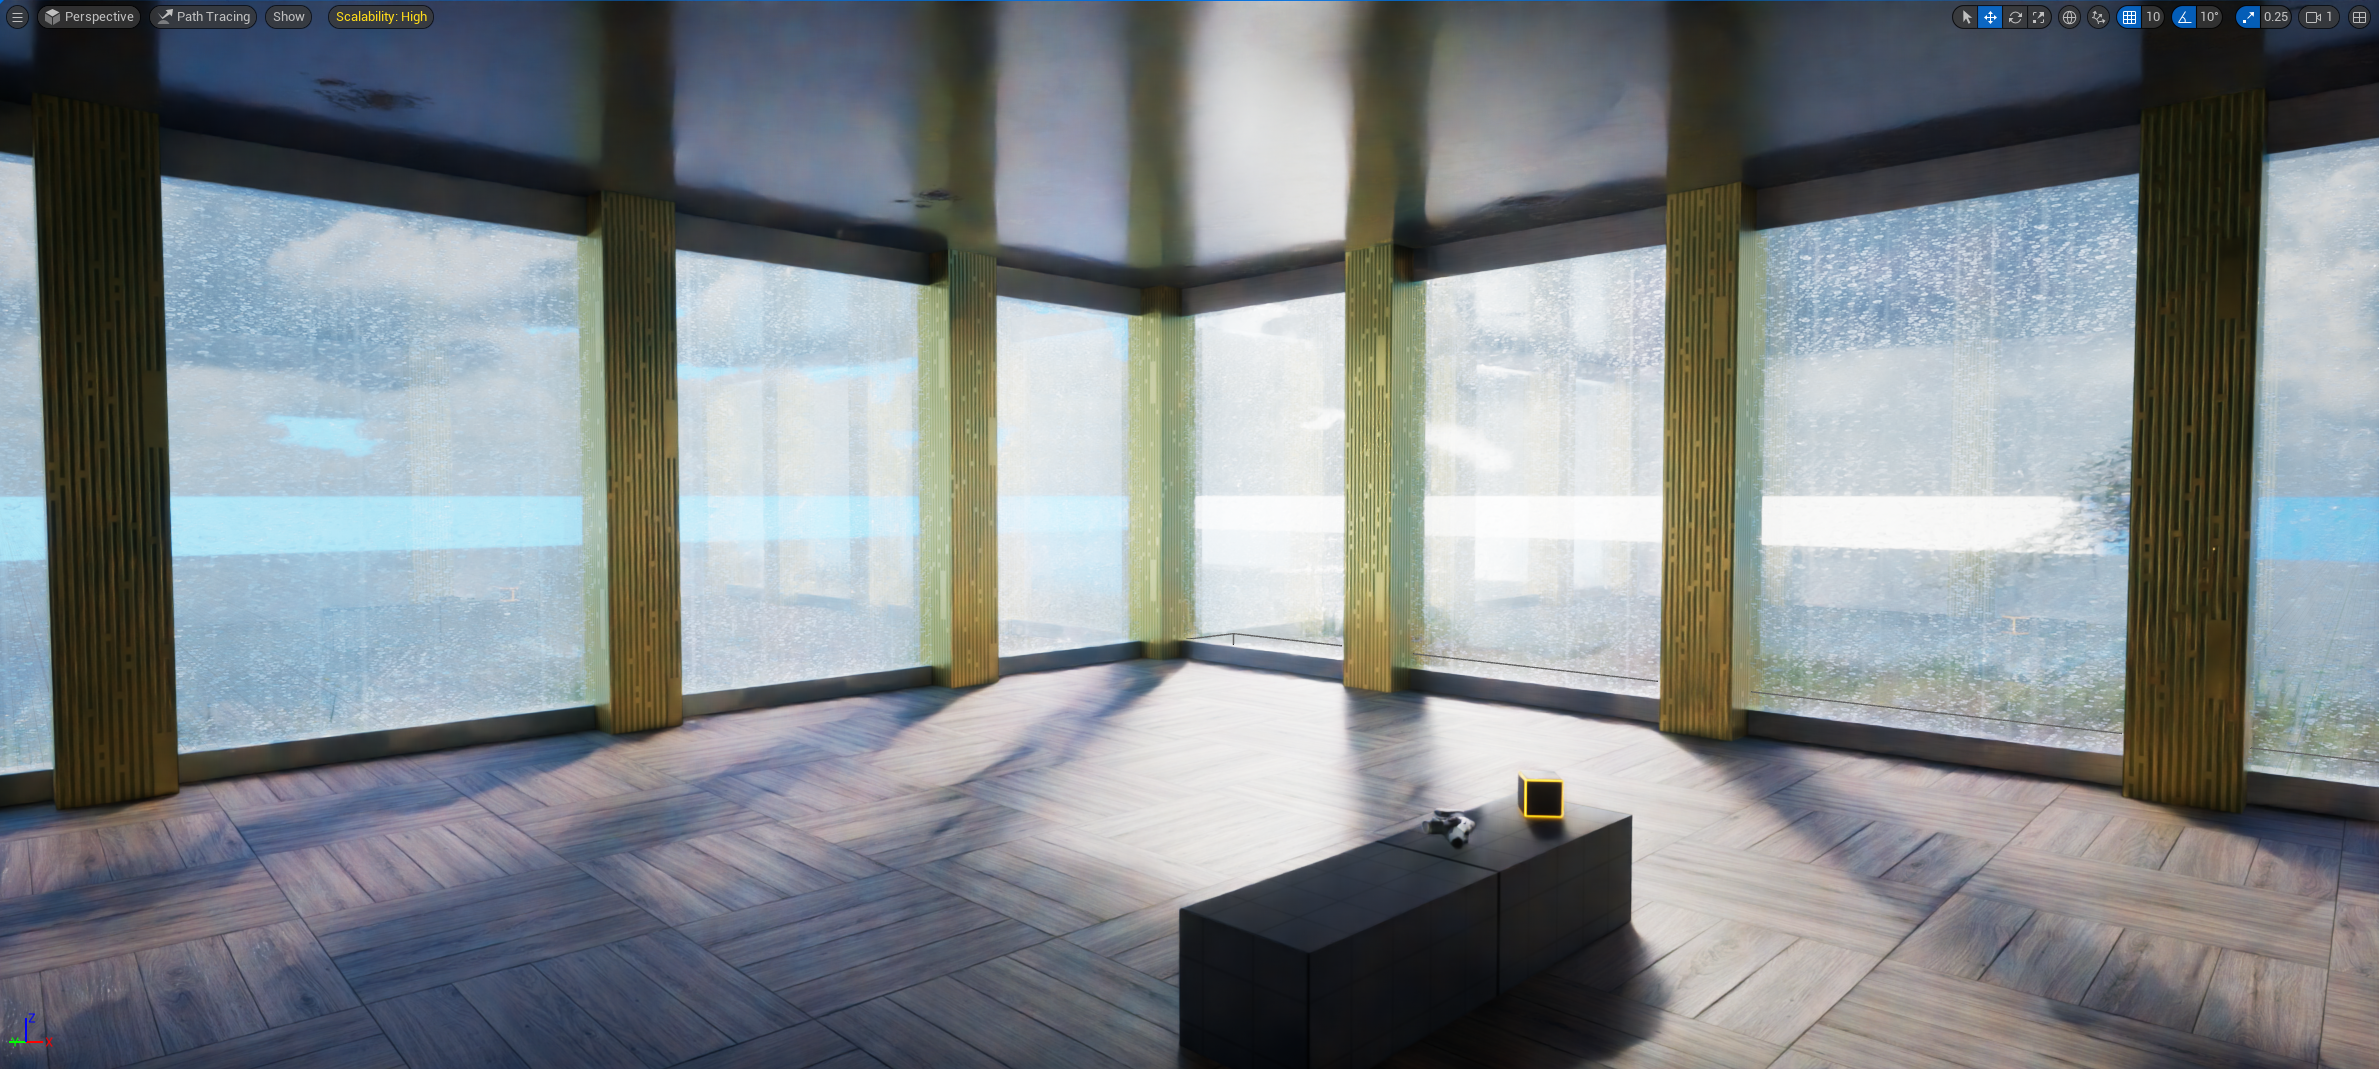
\includegraphics[width=\linewidth, height=6cm]{continut/capitol3/figuri/ray2.png}
        \label{fig:Ray Tracing}
    \end{subfigure}
    \hfill
    \begin{subfigure}{0.49\textwidth}
        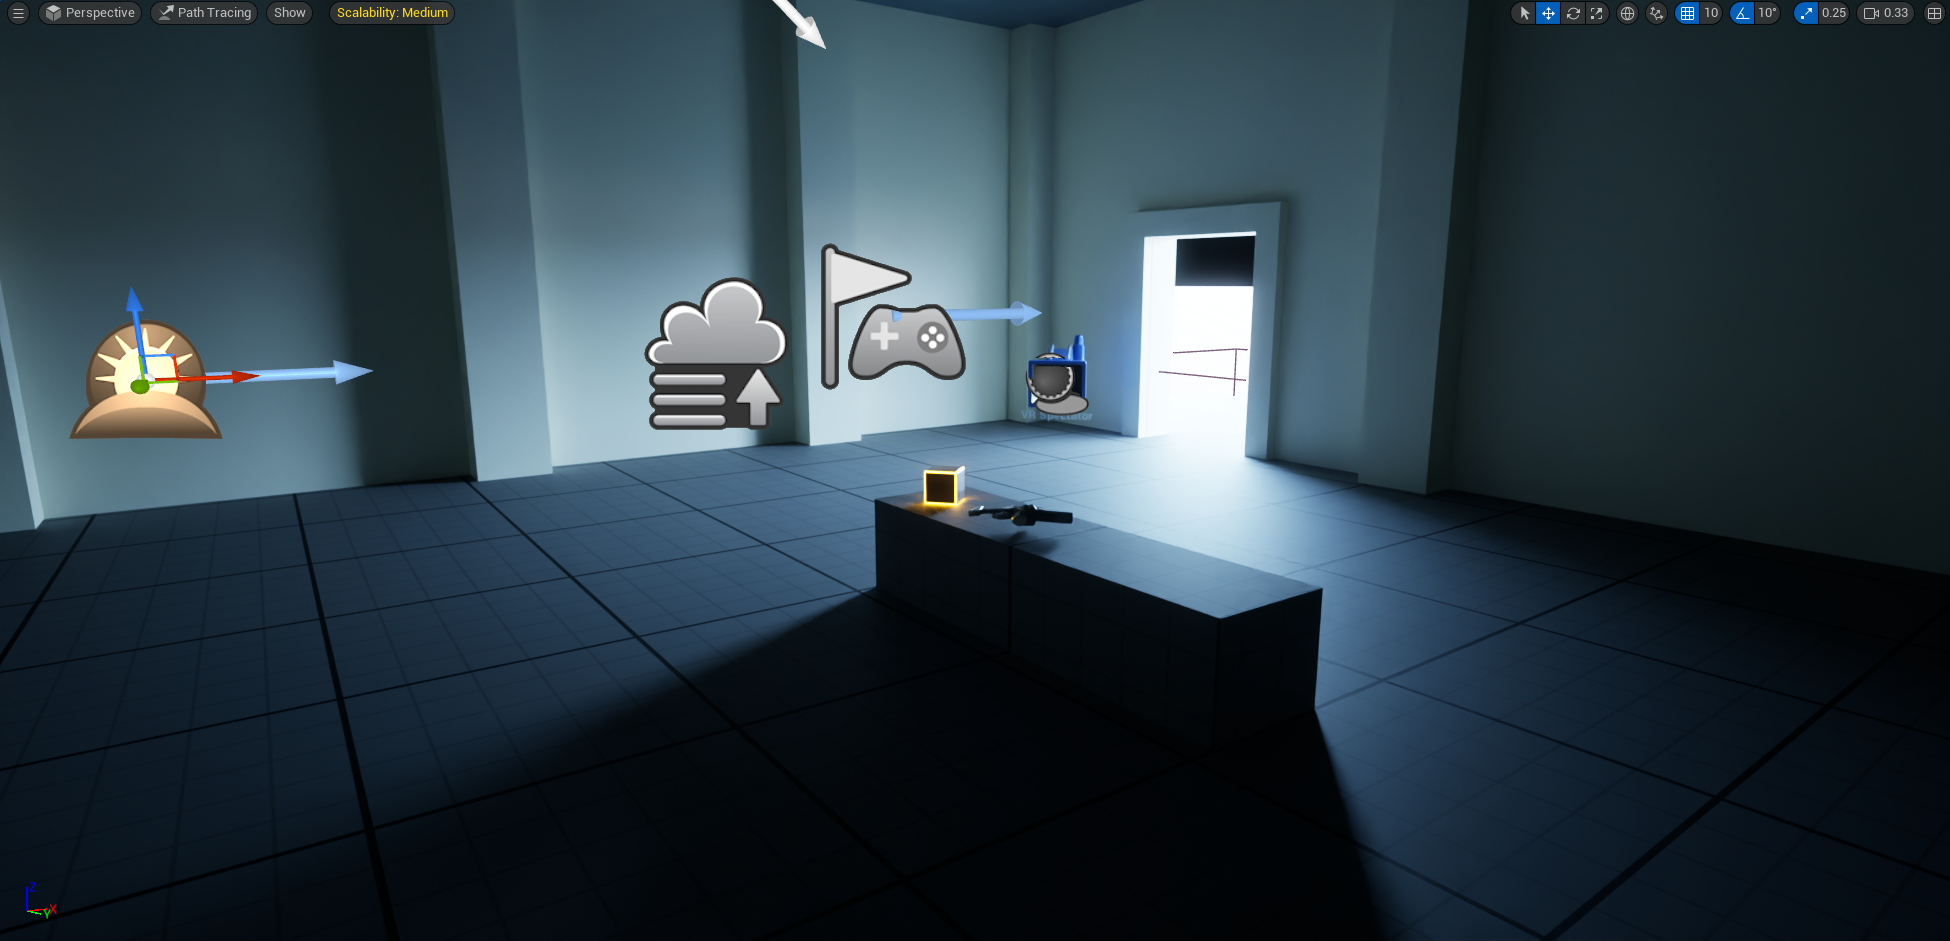
\includegraphics[width=\linewidth, height=6cm]{continut/capitol3/figuri/ray_traced.png}
        \label{fig:Ray Tracing}
    \end{subfigure}
    \caption{Lumina din interior și exterior - teste inițiale}
\end{figure}

În zona exterioară, iluminarea simulează condițiile din timpul amiezii, cu un ambient luminos constant. Soarele este poziționat într-un unghi static optim, astfel încât fiecare model 3D să poată fi observat cu ușurință, fără umbre prea dure sau zone excesiv de întunecate. Nu a fost implementat un ciclu de zi-noapte, deoarece durata medie estimată de explorare a experienței este de aproximativ 10 minute - un interval prea scurt pentru a justifica rotația dinamică a soarelui sau tranziții de iluminare. Astfel, soarele rămâne fix pe cer pe tot parcursul sesiunii.

La interior, arhitectura a fost inițial proiectată cu multe ferestre, însă s-a renunțat ulterior la această soluție în favoarea iluminării artificiale controlate. Ferestrele au fost acoperite parțial sau complet pentru a preveni interferența luminii naturale cu sursele de lumină plasate strategic în muzeu. Astfel, iluminarea interioară se bazează exclusiv pe corpuri de iluminat de tip neon (tuburi fluorescente), amplasate atât deasupra exponatelor, cât și pe tavan.

Această abordare are mai multe avantaje. În primul rând, asigură o distribuție uniformă a luminii, evitând zonele prea întunecate sau prea luminate. În al doilea rând, permite evidențierea efectelor de ray tracing în timp real – reflexii, umbre dinamice și iluminare globală indirectă - care contribuie major la realismul vizual. Fiecare sursă de lumină a fost calibrată pentru a evidenția obiectele din jurul ei, punând accent pe detalii, forme și materiale.

Anumite zone ale muzeului sunt intenționat mai intens luminate pentru a atrage atenția asupra unor expoziții cheie sau pentru a accentua dramatismul scenei. Această variație de intensitate luminează contextul narativ și oferă o experiență mai dinamică.

\begin{figure} [htp] 
\centering 
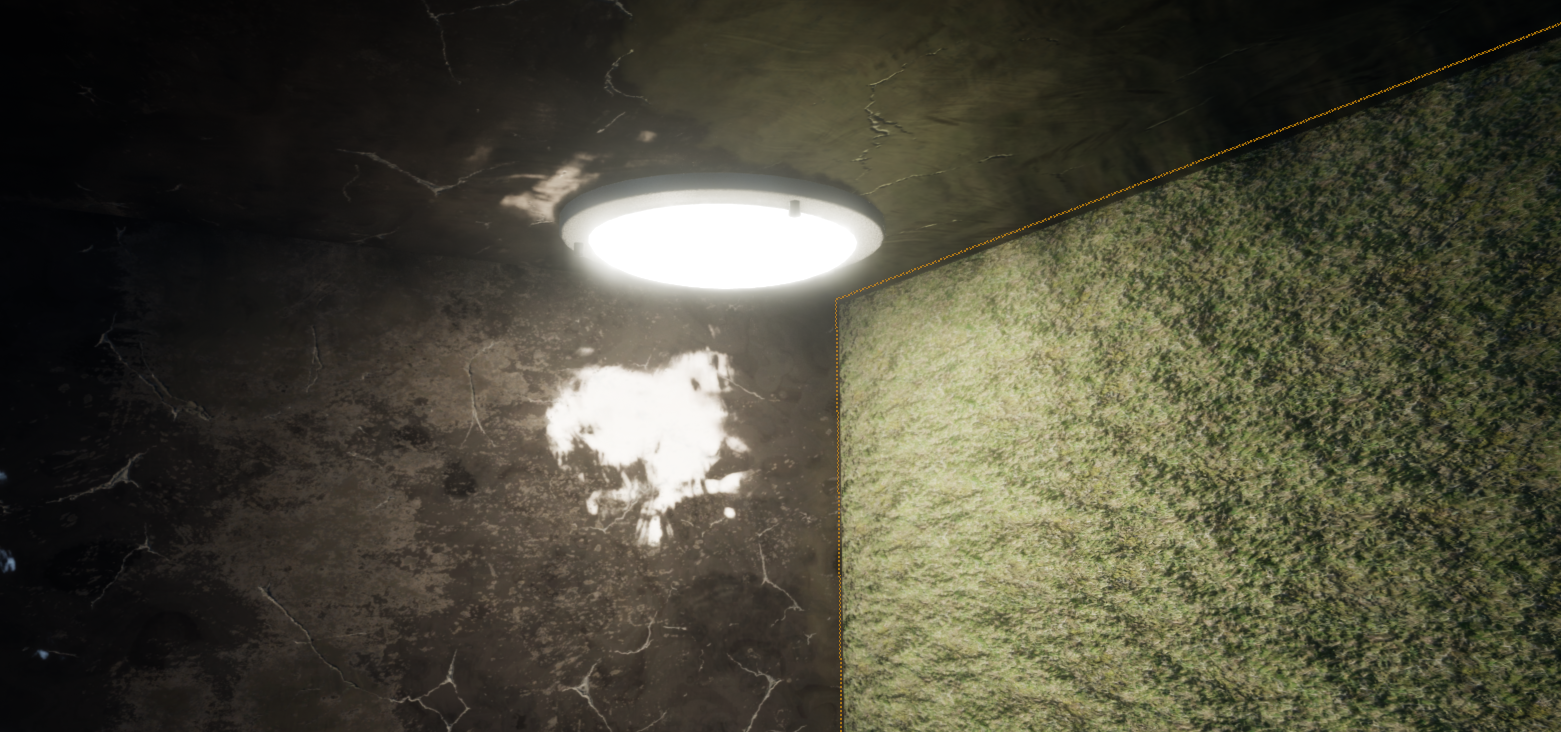
\includegraphics [width=12cm]
{continut/capitol3/figuri/rayBIMtraced.png} 
\label{fig:Ray Tracing} 
    \caption{Ray Tracing}
\end{figure}

Totuși, în unele cazuri pot apărea mici artefacte vizuale, precum flickering-ul luminii (palpitații sau variații neașteptate de intensitate), cauzate de interacțiuni între geometriile scenei și modul în care lumina este calculată în timp real. Astfel de probleme apar rareori și nu afectează semnificativ experiența generală, mai ales că majoritatea situațiilor au fost optimizate în faza de testare.

De menționat că sistemul de iluminare a fost gândit pentru a fi compatibil cu standardele performanței în VR. Deși iluminarea în timp real oferă rezultate vizuale excelente, aceasta poate fi costisitoare din punct de vedere al resurselor, motiv pentru care s-au realizat compromisuri controlate: s-a preferat folosirea static și stationary lights acolo unde a fost posibil, și s-a limitat numărul de surse dinamice per cameră pentru a menține fluiditatea aplicației.

Iluminarea în VR Museum nu are doar un rol funcțional, ci și estetic și educațional, contribuind activ la conturarea atmosferei generale și la accentuarea punctelor de interes din cadrul turului virtual.

\section{Expoziții}

\begin{figure}[h!]
    \centering
    \begin{subfigure}{0.49\textwidth}
        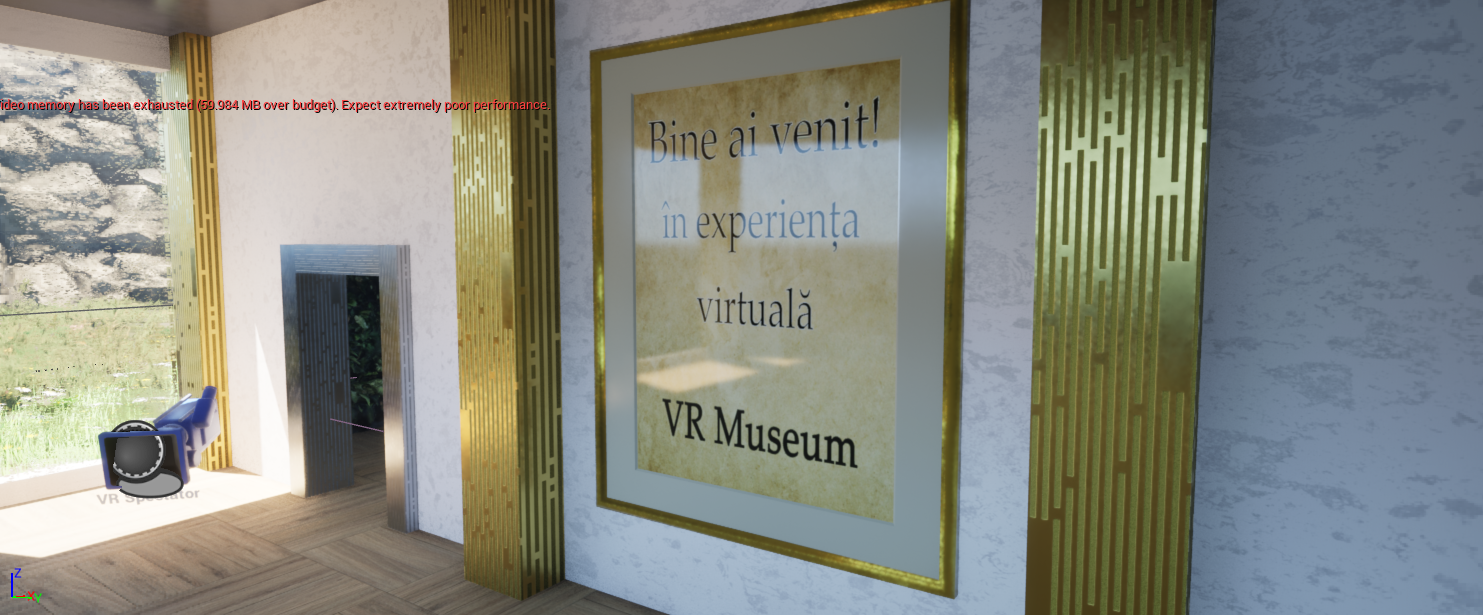
\includegraphics[width=\linewidth, height=6cm]{continut/capitol3/figuri/panel.png}
        \label{fig:Terrain mapping}
    \end{subfigure}
    \hfill
    \begin{subfigure}{0.49\textwidth}
        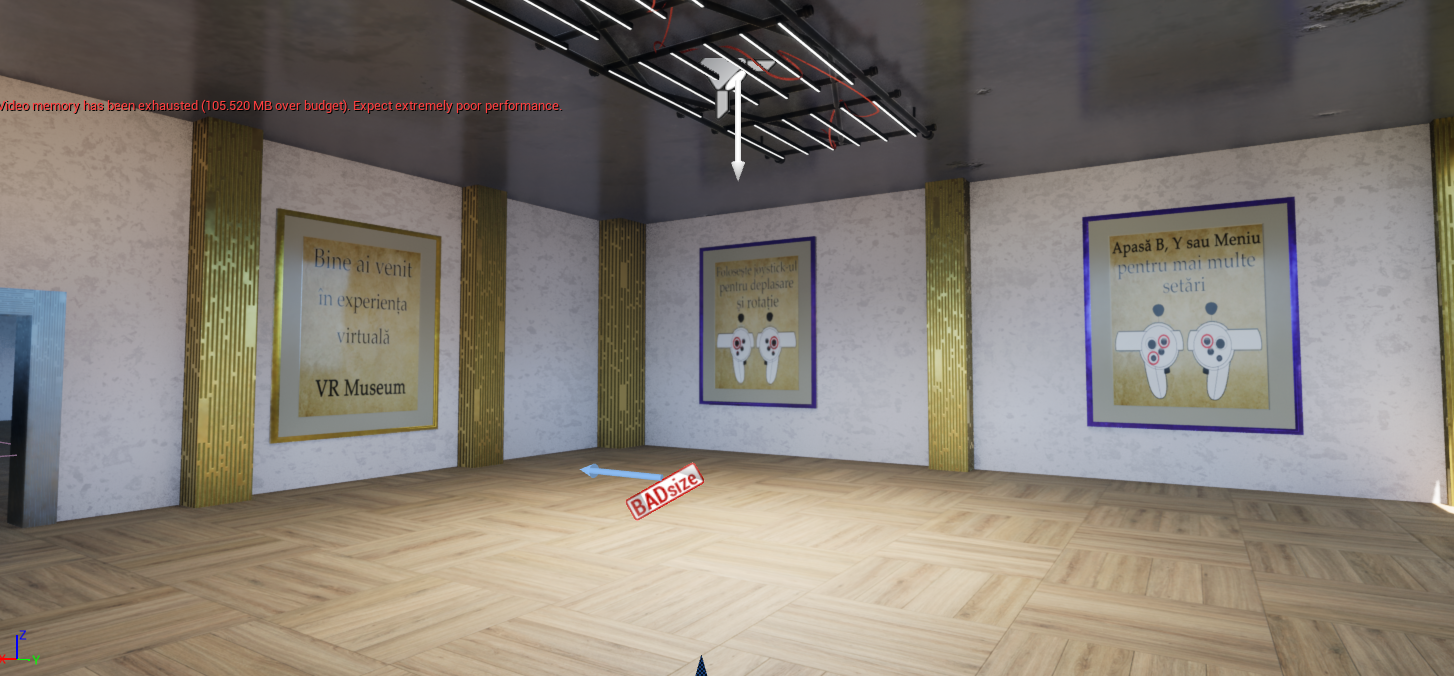
\includegraphics[width=\linewidth, height=6cm]{continut/capitol3/figuri/panel2.png}
        \label{fig:Terrain mapping}
    \end{subfigure}
    \caption{Camera de start}
\end{figure}

În cadrul muzeului virtual sunt integrate mai multe expoziții tematice, fiecare amplasată în încăperi distincte, cu o identitate vizuală și informațională proprie. Distribuția acestora este gândită astfel încât utilizatorul să parcurgă un traseu progresiv, în care imersiunea și gradul de interacțiune cresc odată cu avansarea prin spațiul muzeal.

Camera de inițializare (start room) are rolul de a familiariza utilizatorul cu sistemul de control, printr-o zonă special dedicată testării mișcării, orientării spațiale și interacțiunilor de bază. Aici pot fi observate instrucțiuni vizuale, meniu simplificat și elemente interactive de antrenament, toate într-un mediu neutru, menit să introducă vizitatorul în experiență fără disconfort.

\begin{figure}[h!]
    \centering
    \begin{subfigure}{0.49\textwidth}
        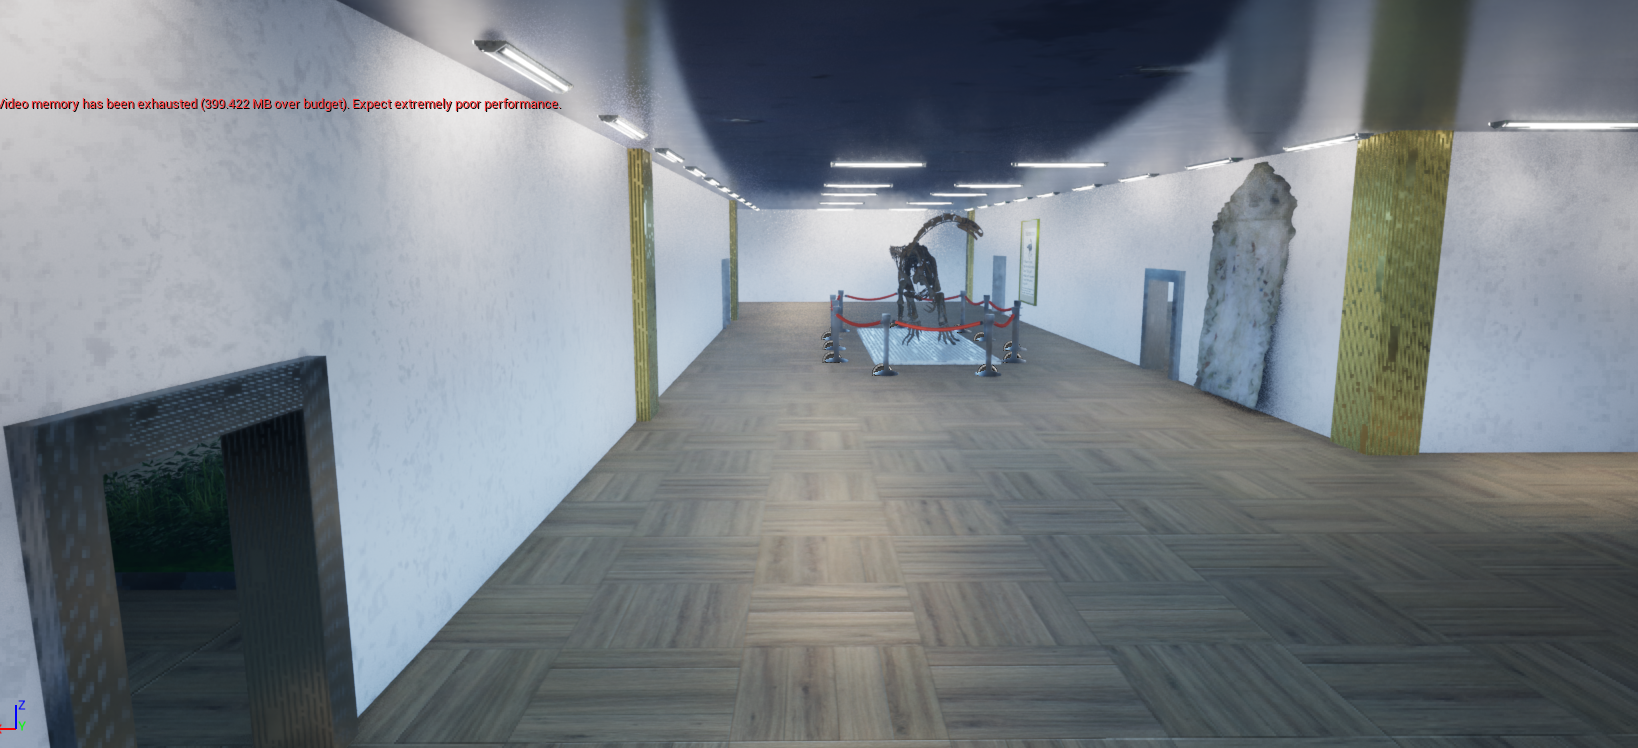
\includegraphics[width=\linewidth, height=6cm]{continut/capitol3/figuri/hol.png}
        \label{fig:Terrain mapping}
    \end{subfigure}
    \hfill
    \begin{subfigure}{0.49\textwidth}
        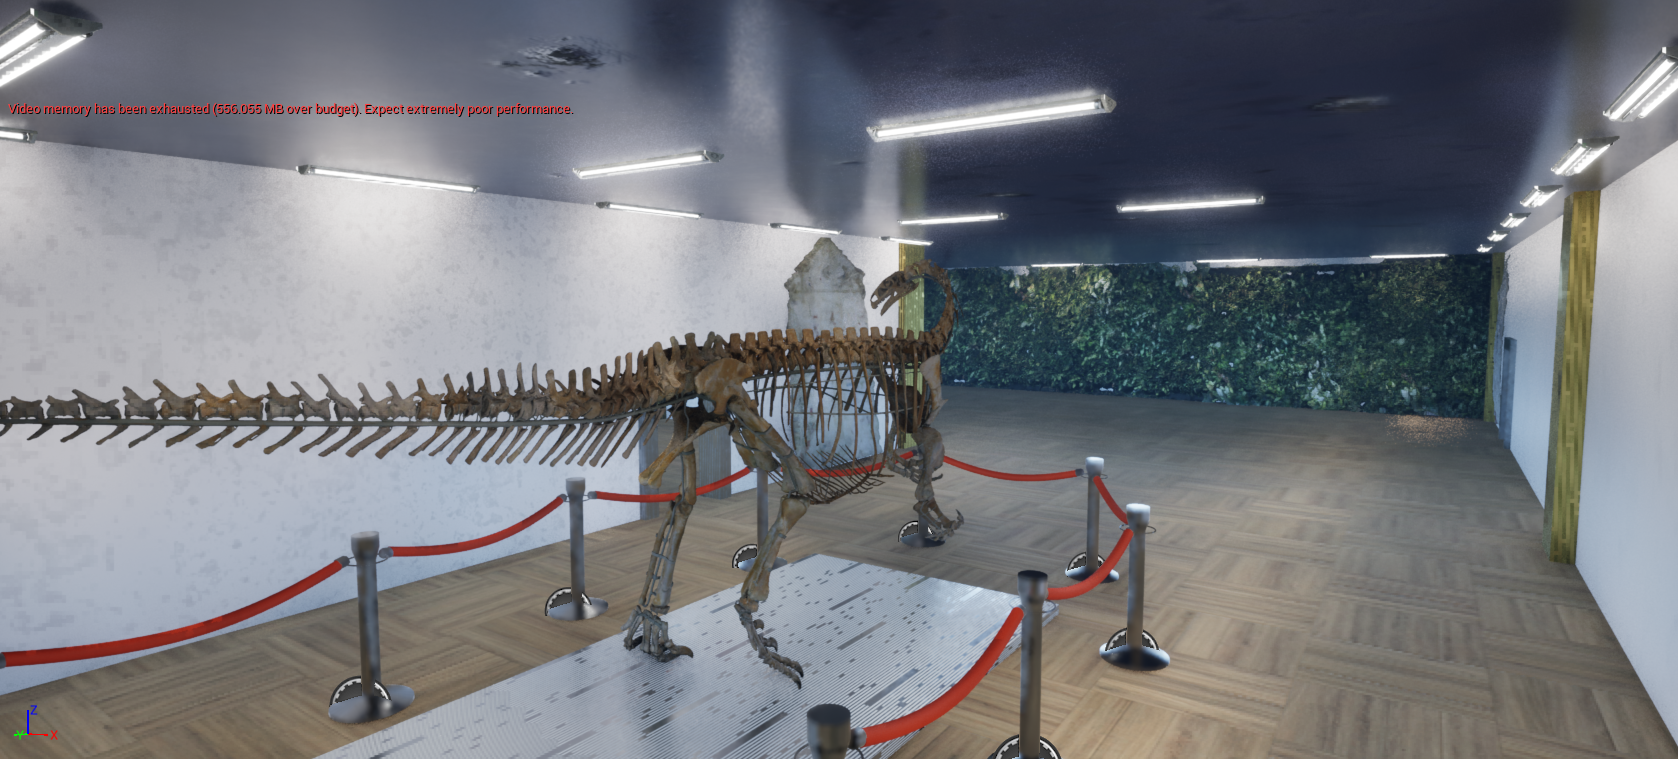
\includegraphics[width=\linewidth, height=6cm]{continut/capitol3/figuri/hol2.png}
        \label{fig:Terrain mapping}
    \end{subfigure}
    \caption{Holul muzeului}
\end{figure}

Urmează holul central, un spațiu amplu decorat cu vegetație 3D, lumină volumetrică și efecte ambientale dinamice. Holul servește drept nod de legătură către celelalte săli și adăpostește o piesă centrală remarcabilă: un schelet de Paleosaurus, modelat cu detalii fine și iluminat cu surse direcționale pentru evidențierea structurii osoase.

\begin{figure}[h!]
    \centering
    \begin{subfigure}{0.49\textwidth}
        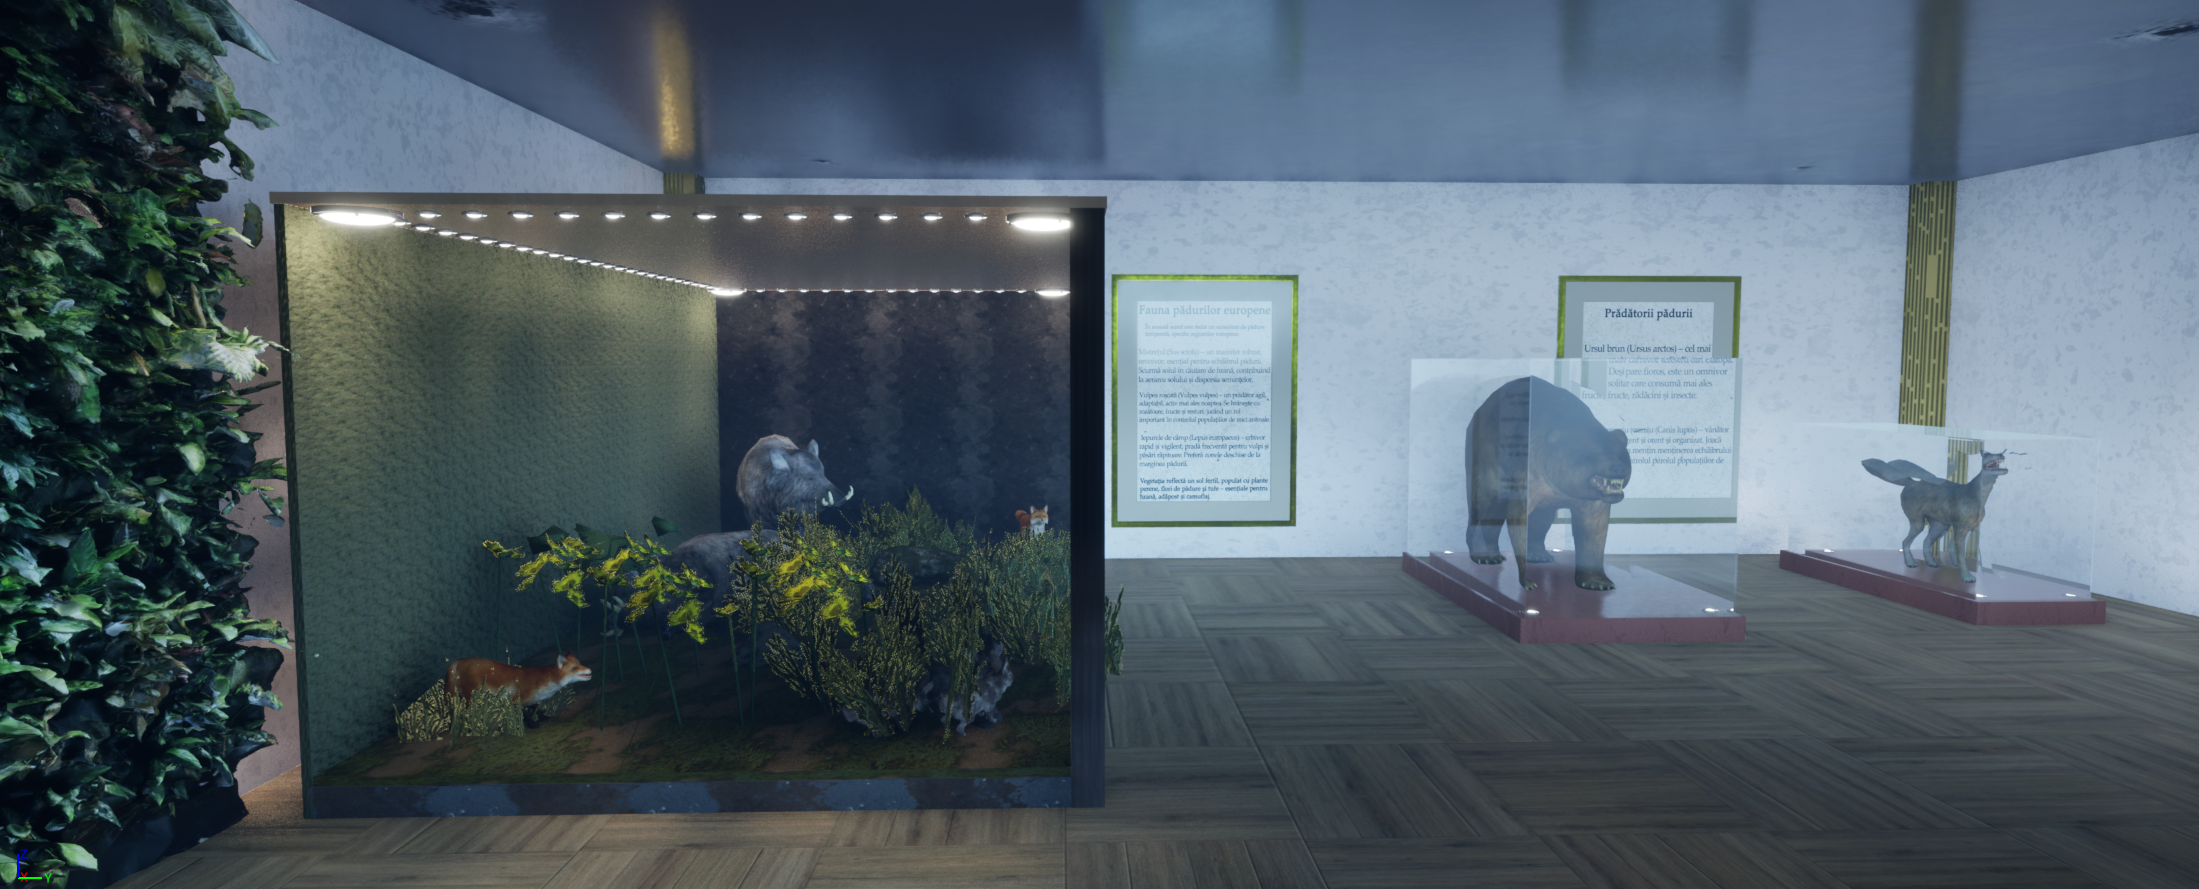
\includegraphics[width=\linewidth, height=6cm]{continut/capitol3/figuri/camera1.png}
        \label{fig:Room1}
    \end{subfigure}
    \hfill
    \begin{subfigure}{0.49\textwidth}
        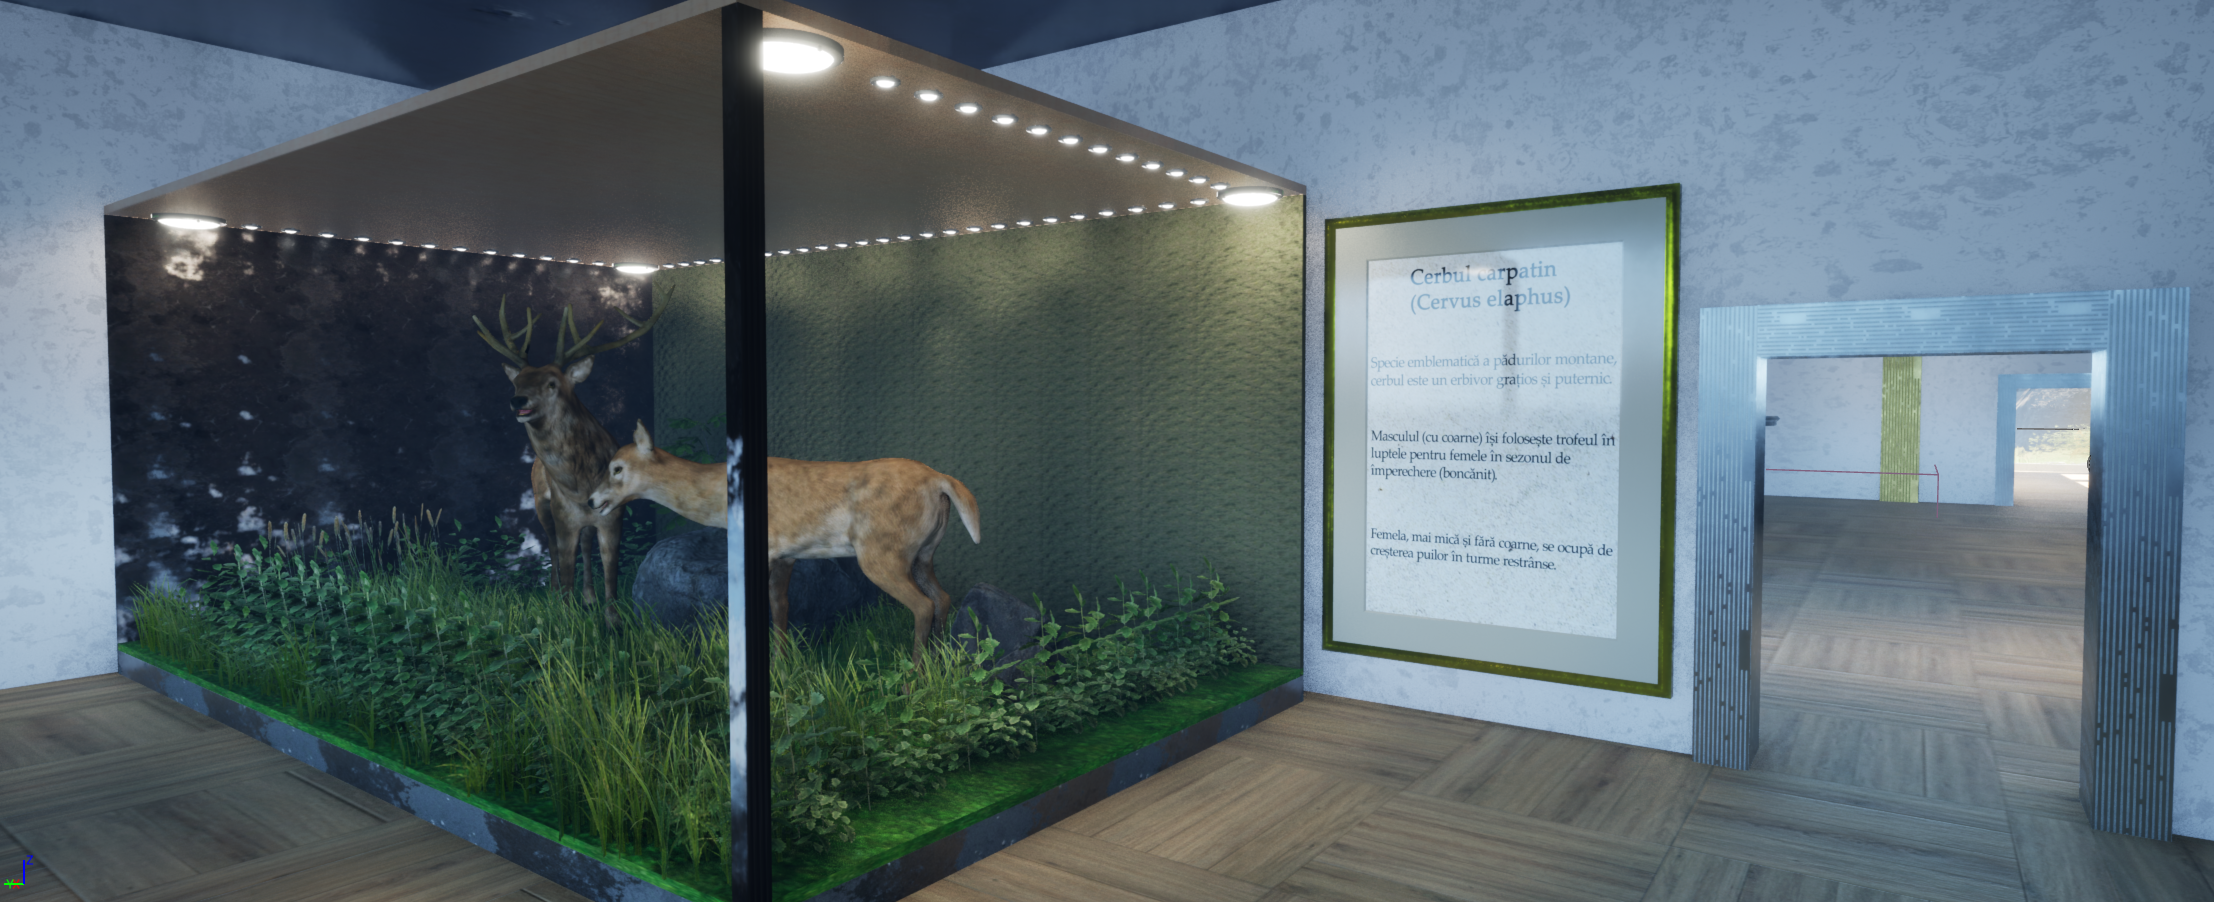
\includegraphics[width=\linewidth, height=6cm]{continut/capitol3/figuri/camera1_2.png}
        \label{fig:Room1}
    \end{subfigure}
    \caption{Camera 1}
\end{figure}

Prima cameră de expoziție este dedicată mamiferelor terestre. Aceasta conține modele 3D realiste ale unor specii sălbatice, atât prădători cât și ierbivore, amplasate în poziții naturale. Fiecare exemplar este însoțit de un panou informativ digital, ce conține date despre habitat, comportament și rolul său în lanțul trofic. Panourile sunt concepute astfel încât informațiile să fie declanșate la apropierea utilizatorului.

\begin{figure}[h!]
    \centering
    \begin{subfigure}{0.49\textwidth}
        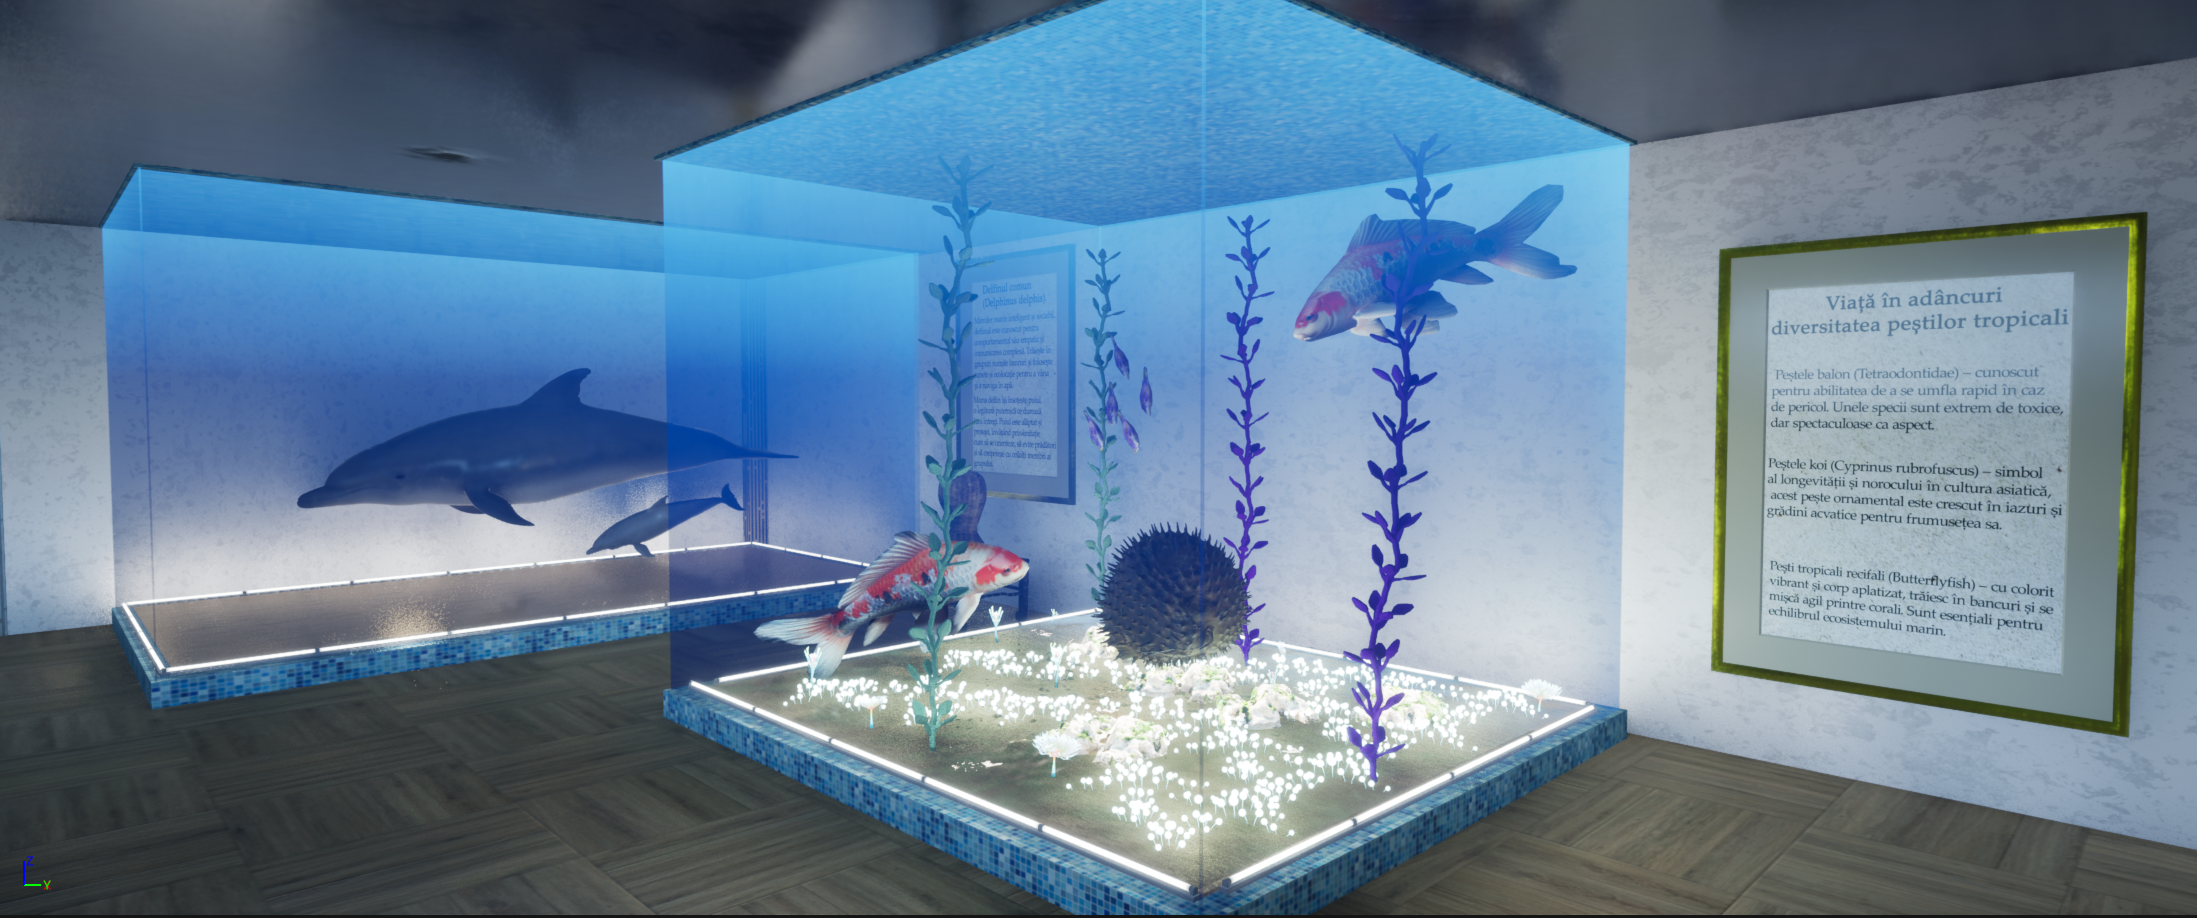
\includegraphics[width=\linewidth, height=6cm]{continut/capitol3/figuri/camera_2.png}
        \label{fig:Room2}
    \end{subfigure}
    \hfill
    \begin{subfigure}{0.49\textwidth}
        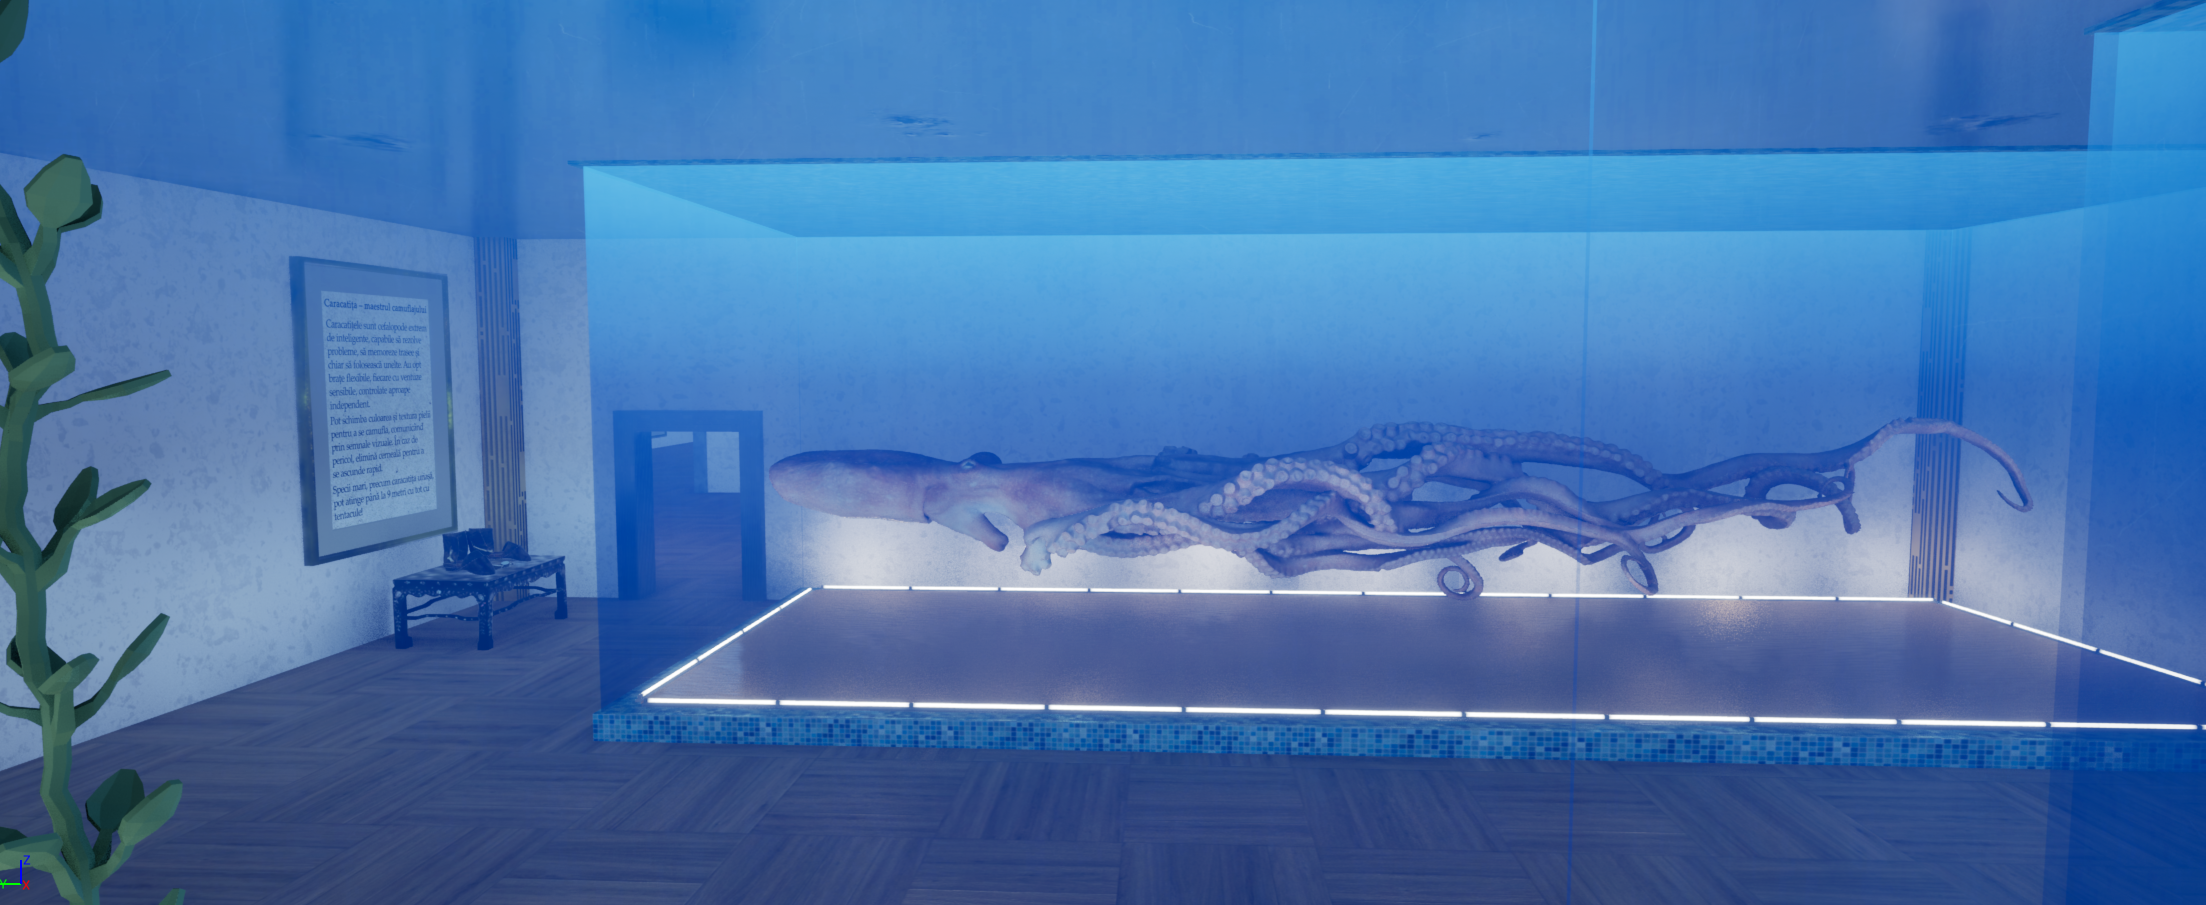
\includegraphics[width=\linewidth, height=6cm]{continut/capitol3/figuri/camera2_2.png}
        \label{fig:Room2}
    \end{subfigure}
    \caption{Camera 2}
\end{figure}

În continuare, camera acvatică oferă o tranziție către mediile subacvatice. Aici pot fi întâlnite un grup familial de delfini (mamă și pui), o caracatiță de dimensiuni mari și un acvariu digital interactiv cu pești tropicali. Pe lângă fauna marină, expoziția include și o serie de obiecte tradiționale folosite în pescuit, precum capcane din lemn, plase vechi și cârlige artizanale, toate recreate digital pe baza surselor istorice.

\newpage 
În partea opusă se află o încăpere mai spațioasă, destinată unei colecții de obiecte istorice de utilitate practică: unelte, recipiente, instrumente de vânătoare și chiar obiecte de divertisment arhaice. Acestea nu sunt prezentate la scară reală, ci au fost redimensionate pentru o mai bună lizibilitate și încadrare vizuală în spațiul VR. Obiectele sunt grupate tematic, fiecare fiind însoțit de o scurtă descriere contextuală – unele cu fundal audio explicativ.

\begin{figure} [htp] 
\centering 
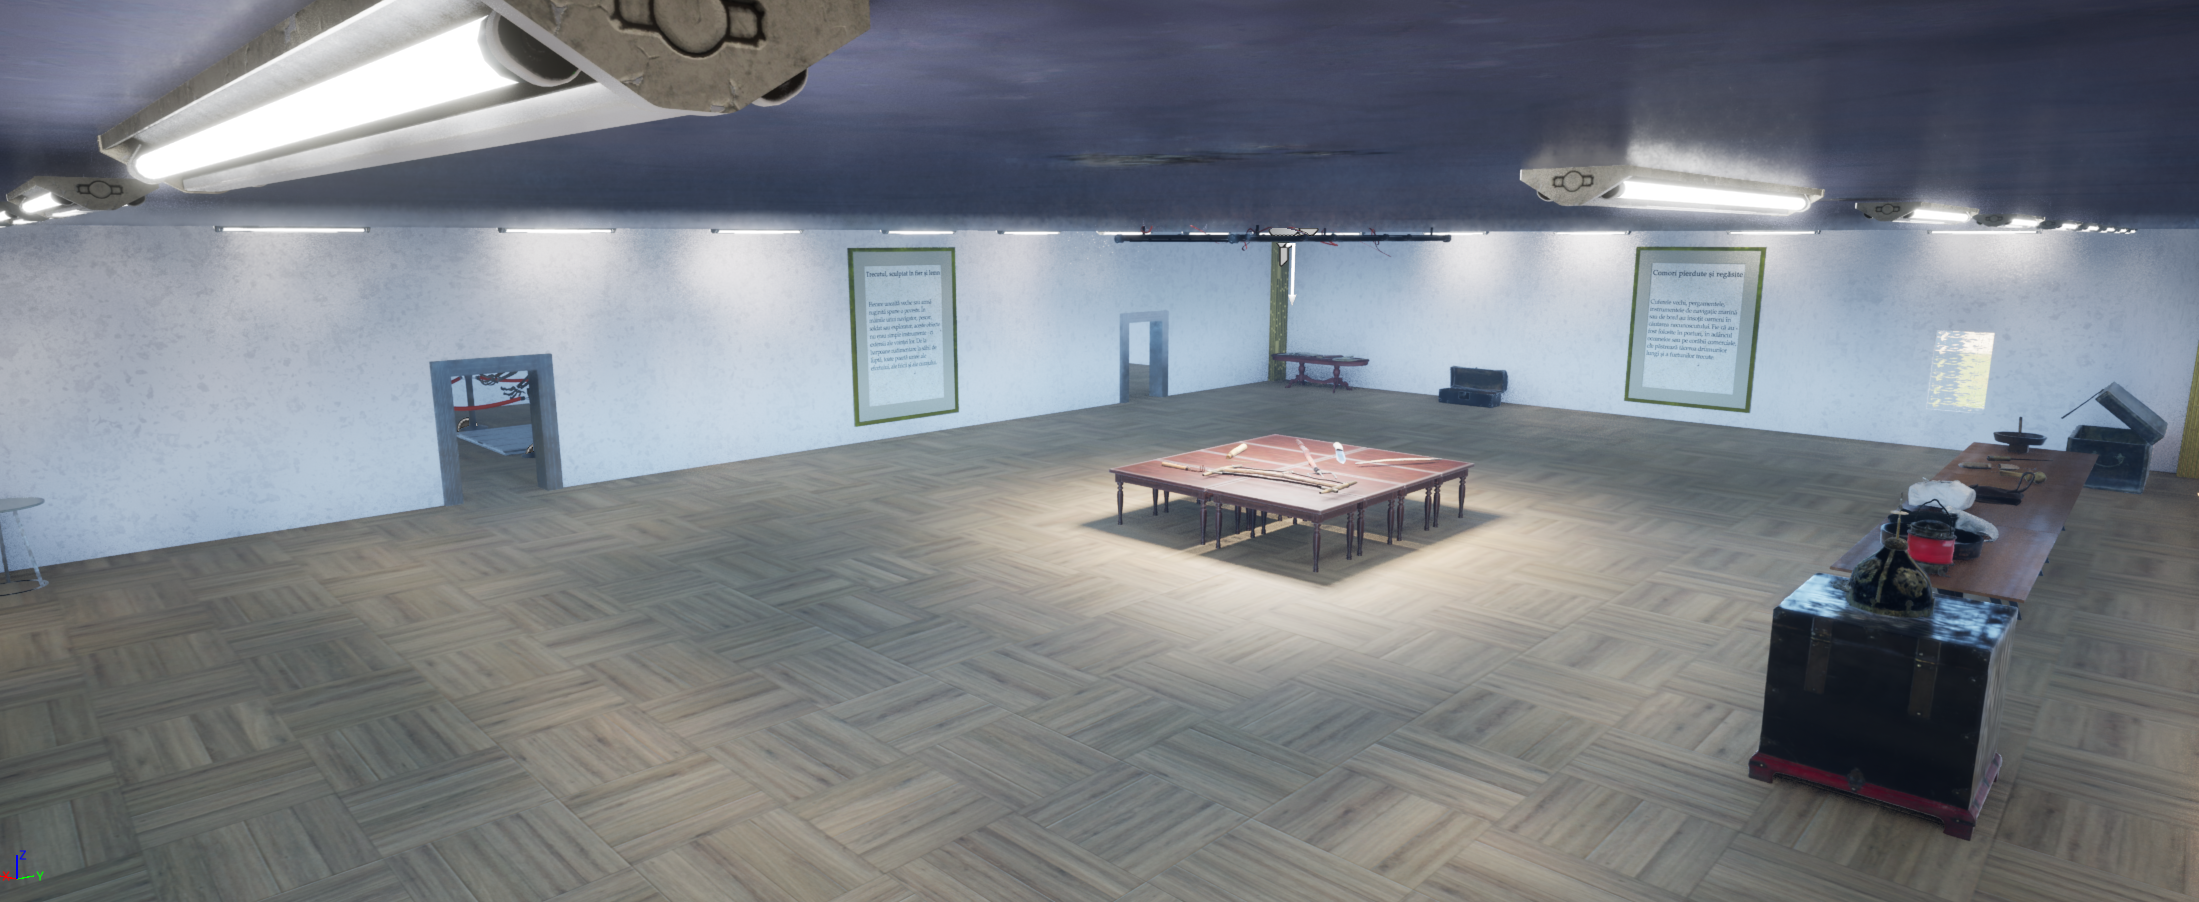
\includegraphics [width=12cm]
{continut/capitol3/figuri/iteme.png} 
\label{fig:Room3} 
    \caption{Camera 3}
\end{figure}

În zona exterioară a muzeului, sunt amplasate exponate de mari dimensiuni care nu puteau fi încadrate în sălile interioare: dinozauri de tip erbivor și carnivor, reconstituiți digital. Fiecare model este acompaniat de o placă informativă și animat în poziție naturală, pentru a reda dinamism. În apropiere se regăsește și o scenă de reproducere, unde este prezentat un cuib cu ouă, din care pot fi observați pui de dinozaur aflați în proces de eclozare – un detaliu menit să aducă un plus de viață și realism.

Toate aceste expoziții au fost create, configurate și ajustate manual, utilizând asset-uri de înaltă calitate, modificate pentru a se potrivi specificului aplicației. S-a acordat o atenție deosebită compoziției scenice, proporțiilor, iluminării și detaliilor – pentru a oferi o experiență personalizată, realistă și educativă. Integrarea fiecărui element s-a făcut cu respectarea cerințelor de performanță în VR, păstrând un echilibru între fidelitatea vizuală și fluiditatea navigării.

\begin{figure}[h!]
    \centering
    \begin{subfigure}{0.49\textwidth}
        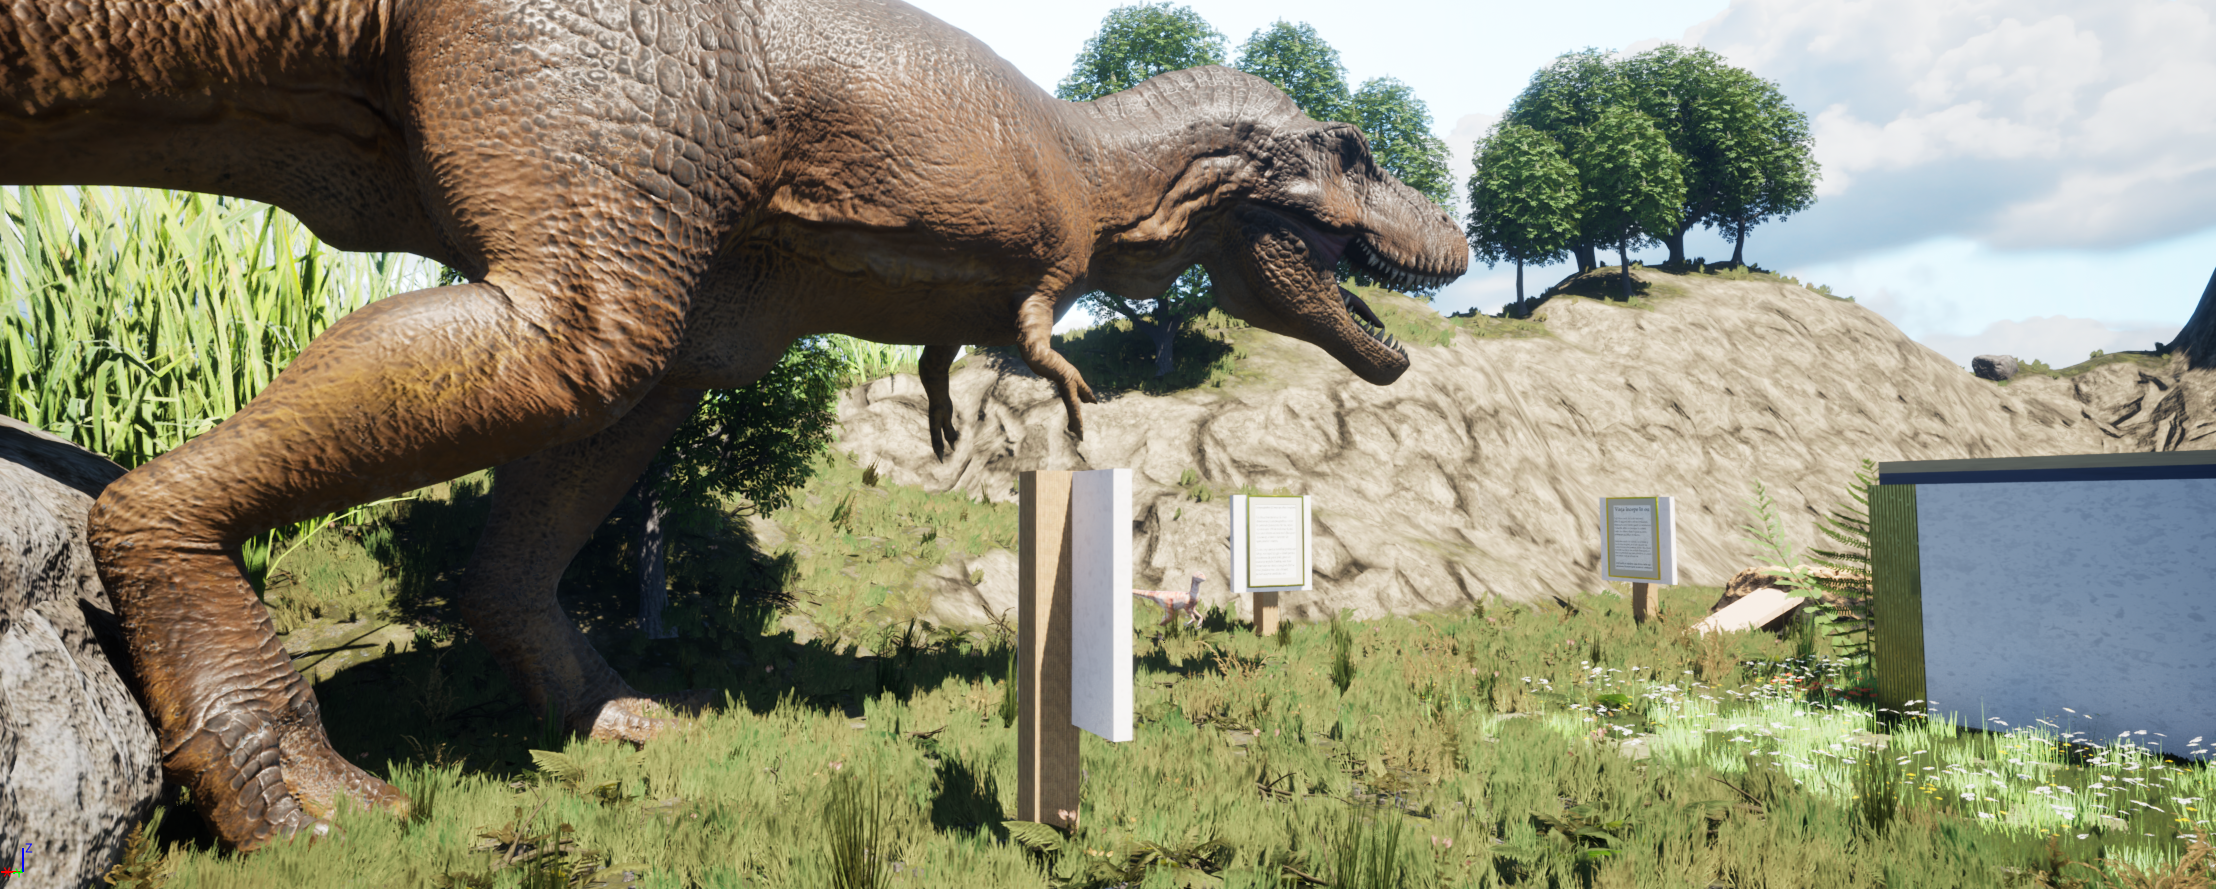
\includegraphics[width=\linewidth, height=6cm]{continut/capitol3/figuri/afara.png}
        \label{fig:outside}
    \end{subfigure}
    \hfill
    \begin{subfigure}{0.49\textwidth}
        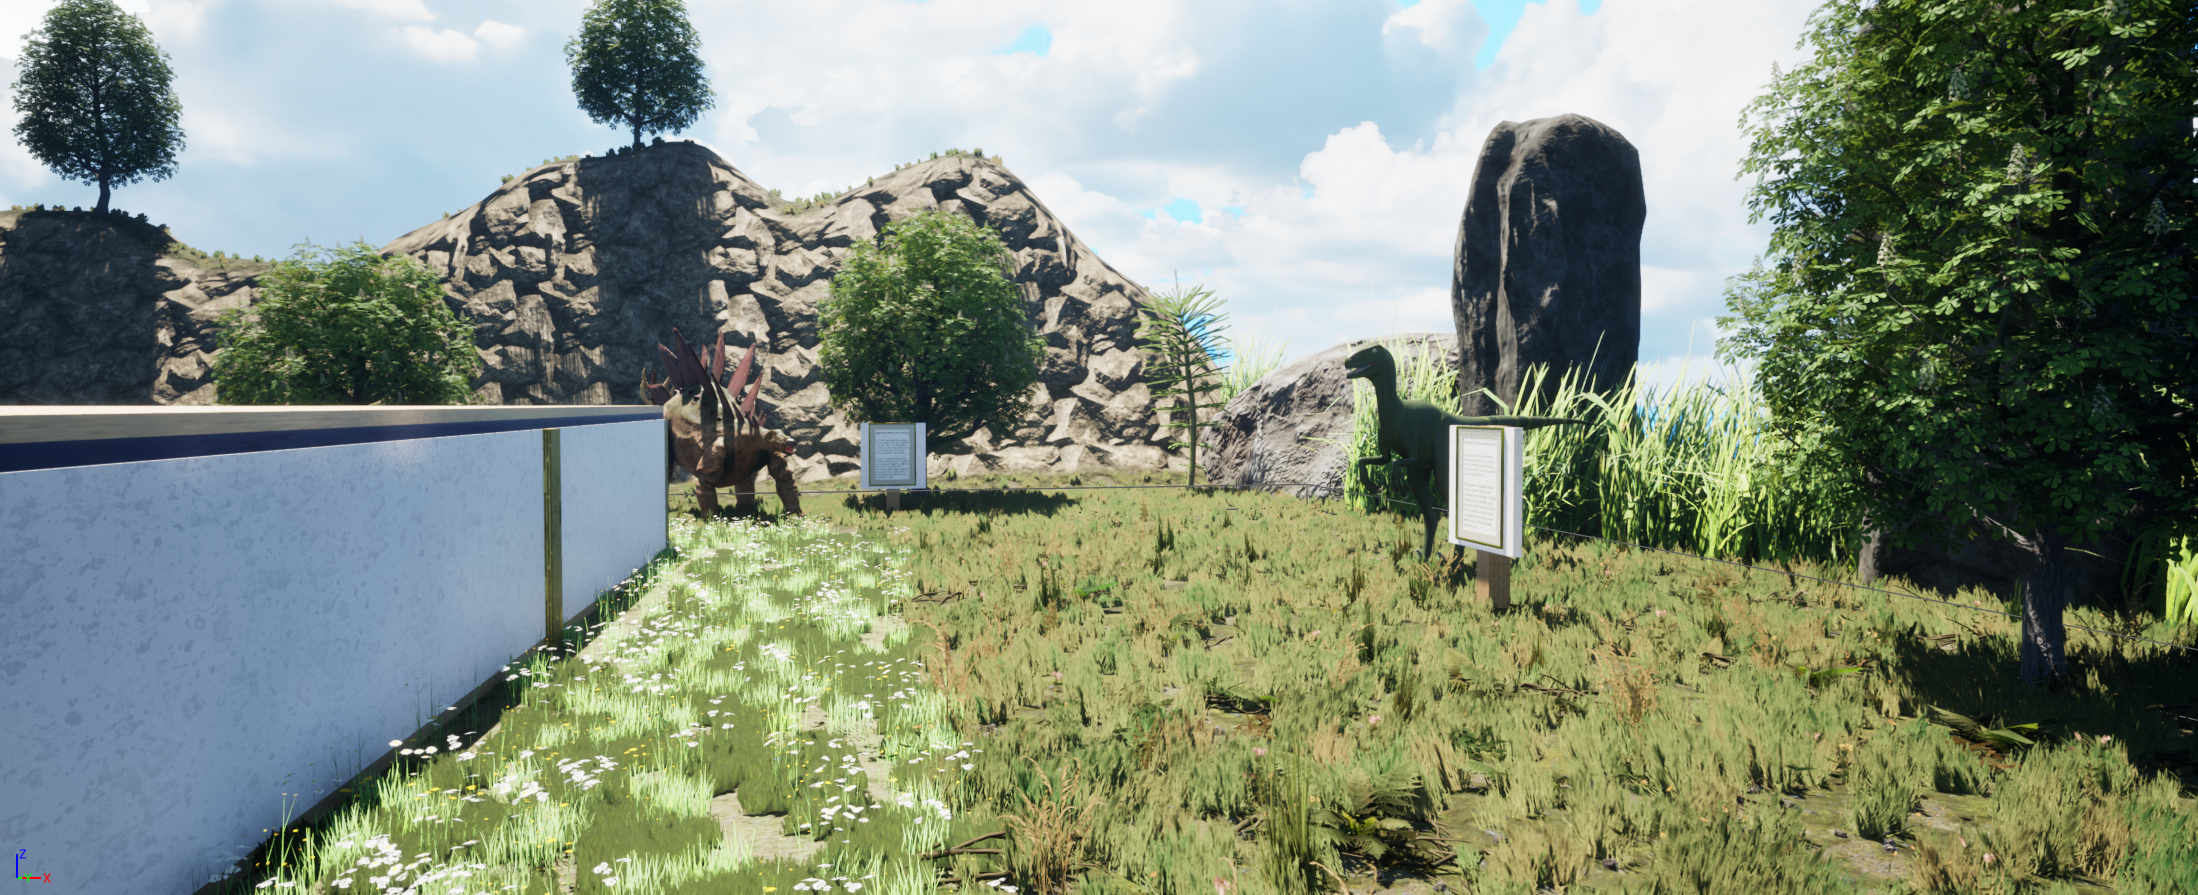
\includegraphics[width=\linewidth, height=6cm]{continut/capitol3/figuri/afara2.png}
        \label{fig:outside}
    \end{subfigure}
    \caption{Muzeul exterior}
\end{figure}

\newpage 

\section{VR Pawn}

Personajul controlat de utilizator în cadrul aplicației VR Museum poartă denumirea de VR Pawn, o componentă fundamentală în dezvoltarea oricărei aplicații compatibile cu realitatea virtuală în Unreal Engine. Spre deosebire de clasa standard de „Player Character” folosită în jocurile de tip First-Person sau Third-Person, unde controlul este limitat la mișcare și cameră, în cazul realității virtuale, interacțiunea se extinde la un nivel mult mai granular, incluzând urmărirea mâinilor, mișcarea independentă a acestora și detecția coliziunilor sau a gesturilor în spațiu.

În contextul aplicației dezvoltate, VR Pawn are un rol central în structură, întrucât majoritatea funcționalităților sunt gestionate local, aplicația fiind una single-player și rulând direct pe sistemul utilizatorului. Astfel, VR Pawn devine nucleul logicii aplicației, acționând nu doar ca intermediar între utilizator și scenă, ci și ca element de legătură („bridge”) între multiple module funcționale.

Printre componentele critice integrate în cadrul VR Pawn-ului se numără, printre altele, meniul principal al aplicației și sistemul de locomotion (deplasare), fiecare dintre acestea având o implementare complexă, ce va fi detaliată în secțiunile următoare.

\begin{figure} [htp] 
\centering 
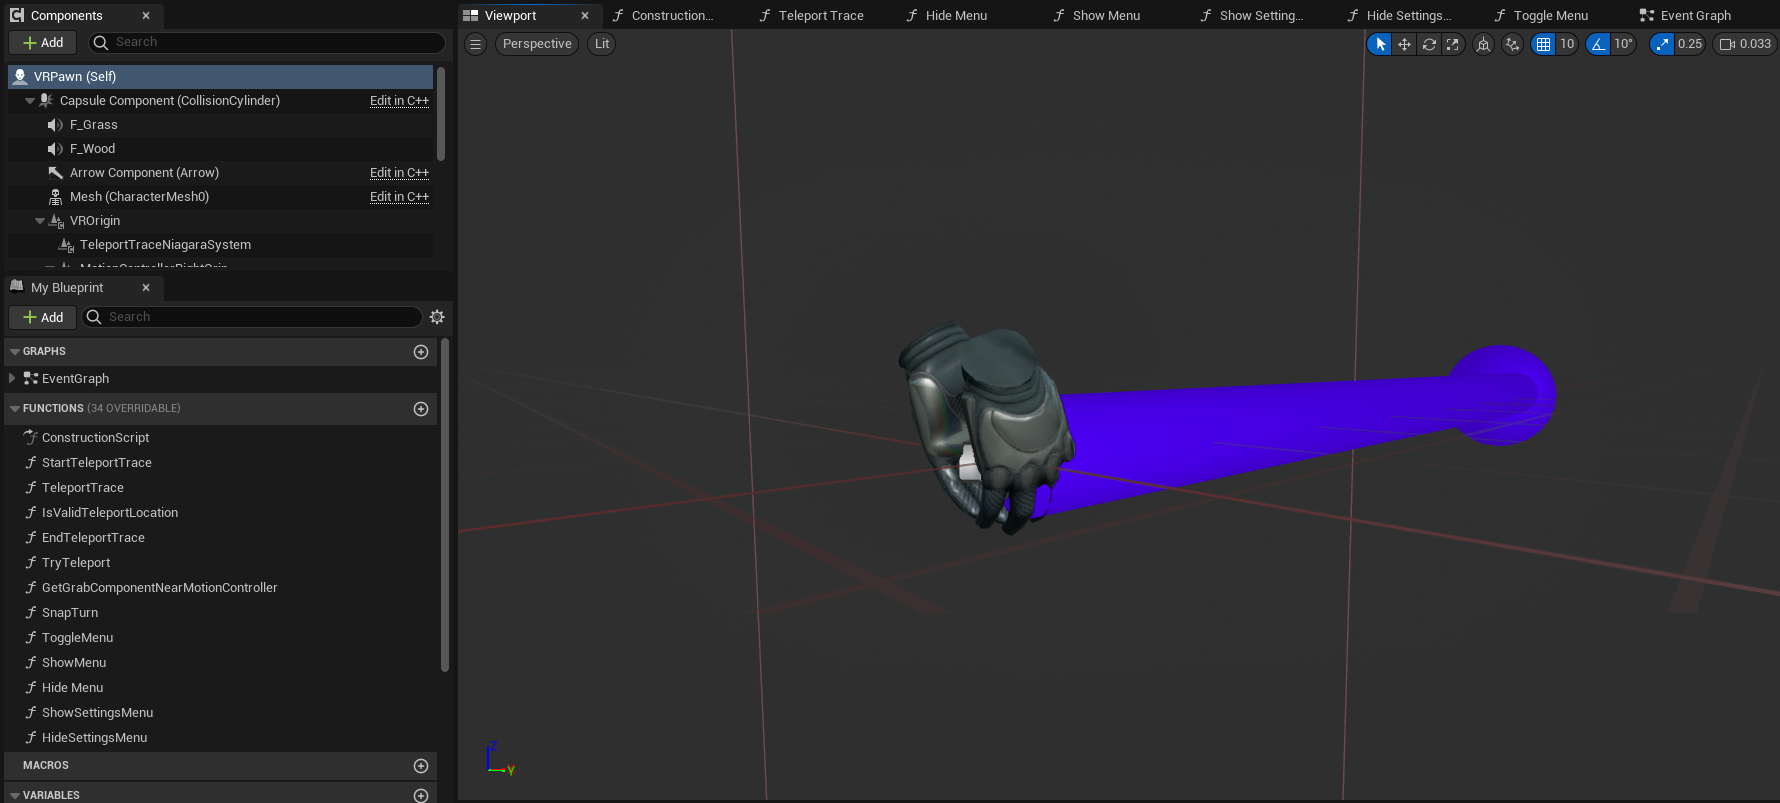
\includegraphics [width=12cm]
{continut/capitol3/figuri/VR_Pawn.png} 
\label{fig:VR_Pawn} 
    \caption{VR Pawn}
\end{figure}

\section{Movement}

În versiunea originală a șablonului Virtual Reality Template, este prezent un sistem de locomoție de bază, bazat pe teleportare. Această metodă este frecvent utilizată în aplicații VR datorită avantajelor legate de confortul utilizatorului, reducând riscul de motion sickness. Cu toate acestea, implementarea oferită în template-ul implicit este destul de rudimentară și prezintă mai multe limitări atât din punct de vedere tehnic, cât și vizual.

Mai exact, sistemul de teleportare nu detectează întotdeauna corect suprafețele valide pentru deplasare. Ray-ul proiectat din controller intersectează uneori plane verticale sau obiecte neadecvate (precum margini de mesh-uri), iar zona de destinație poate deveni confuză pentru utilizator. În plus, efectele vizuale asociate teleportării sunt minime: indicatorul de plasare este static și lipsit de feedback clar, ceea ce diminuează experiența de utilizare și poate crea incertitudine privind punctul exact de sosire.

Pentru a îmbunătăți calitatea și naturalețea deplasării în mediul virtual, se apelează la un sistem de locomoție continuă, atât pentru deplasarea liniară (smooth locomotion), cât și pentru rotație (smooth turn). Această metodă oferă un control mai precis și o experiență mai apropiată de explorarea din lumea reală, fiind mai potrivită pentru un tur virtual al unui muzeu.

Noua metodă se bazează pe interpretarea semnalului analogic de la joystick-uri:
\begin{itemize}
\item Joystick-ul stâng controlează direcția de deplasare, permițând utilizatorului să meargă înainte, înapoi sau lateral, în funcție de orientarea sa;
\item Joystick-ul drept controlează rotația continuă, cu o viteză definită în funcție de intensitatea devierii.
\end{itemize}

Pentru a implementa sistemul de locomoție continuă în cadrul experienței VR, au fost introduse două funcții noi mapate pe joystick-urile controlerelor, utilizând sistemul Enhanced Input Action din Unreal Engine 5. Aceste funcții sunt: SmoothMove si SmoothTurn

\textbf{SmoothMove:}

Funcționalitatea de deplasare continuă presupune mai multe componente care lucrează împreună, dintre care cele mai importante sunt: determinarea direcției de mișcare, detectarea suprafeței și redarea pașilor.

\begin{figure} [htp] 
\centering 
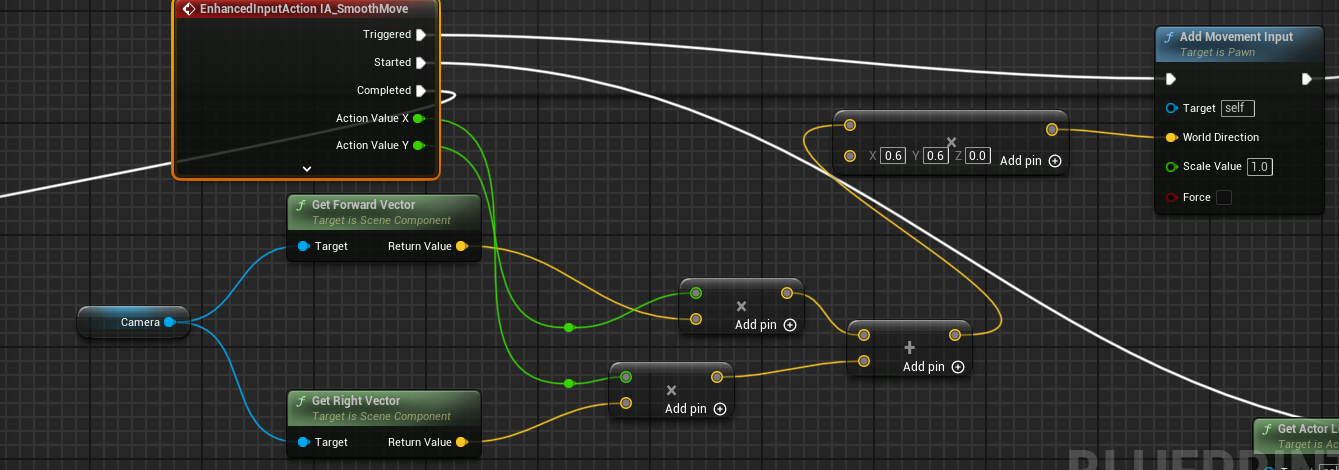
\includegraphics [width=12cm]
{continut/capitol3/figuri/SmoothMove.png} 
\label{fig:VR_Pawn} 
    \caption{Smooth Move}
\end{figure}

Pentru ca deplasarea să fie realistă și corect orientată, este necesară obținerea coordonatelor actorului (VRPawn) și a direcției sale de privire. Aceste informații sunt esențiale pentru a calcula vectorii de mișcare pe axele înainte și lateral (forward și right).

Camera atașată Pawn-ului VR este utilizată pentru a extrage vectorii de orientare prin funcțiile GetForwardVector și GetRightVector. Acești vectori sunt ulterior înmulțiți cu valorile analogice provenite de la joystick (care indică direcția și intensitatea mișcării). Vectorul rezultat este transmis ca parametru către funcția AddMovementInput, care aplică mișcarea în sistemul de coordonate global (World Direction), asigurând o deplasare fluidă și direcționată corect.

Surface Detection și efecte audio: Footsteps
Pentru a spori realismul experienței, a fost integrat un sistem audio care redă sunete de pași diferiți în funcție de suprafața pe care se deplasează utilizatorul.

Au fost selectate efecte sonore din biblioteca Epidemic Sound, grupate în două categorii principale:
\begin{itemize}
\item \textbf{ParquetCore} - care conține 22 de sunete de pași pe podea de lemn
\item \textbf{GrassCore} - cuprinzând 15 sunete de pași pe suprafețe naturale, cum ar fi pământ și iarbă
\end{itemize}

\begin{figure}[h!]
    \centering
    \begin{subfigure}{0.49\textwidth}
        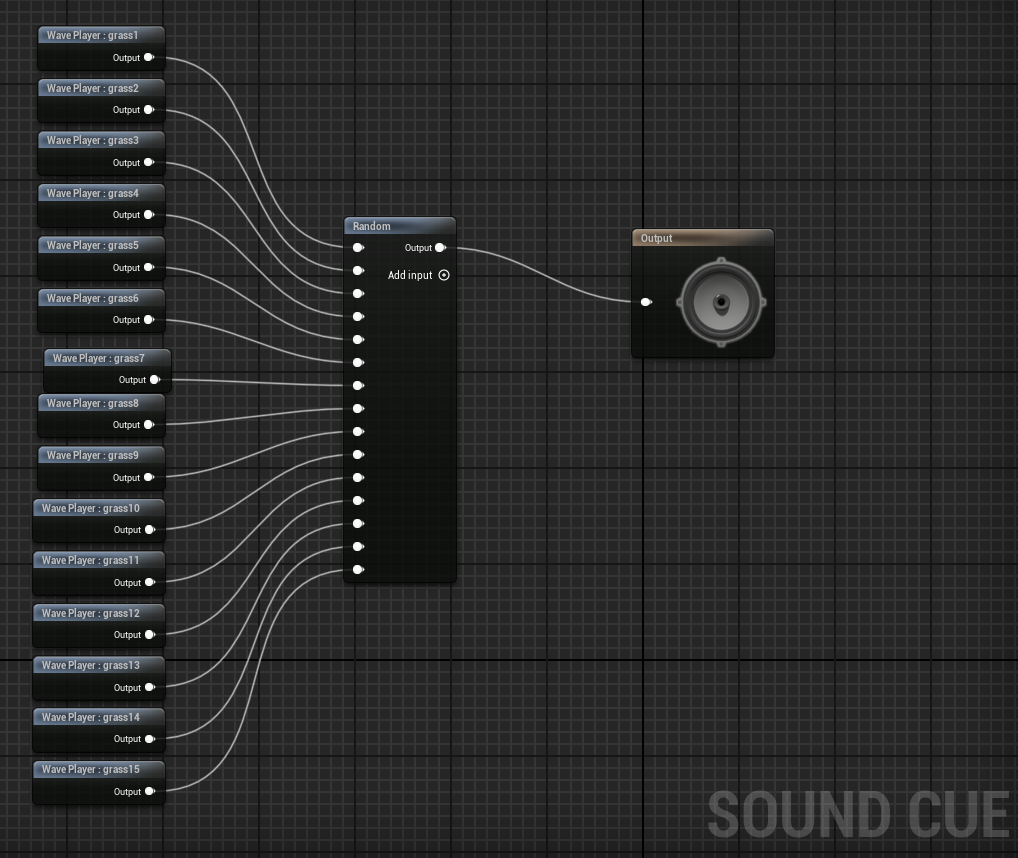
\includegraphics[width=\linewidth, height=6cm]{continut/capitol3/figuri/step_grass.png}
        \label{fig:VR_Pawn}
    \end{subfigure}
    \hfill
    \begin{subfigure}{0.49\textwidth}
        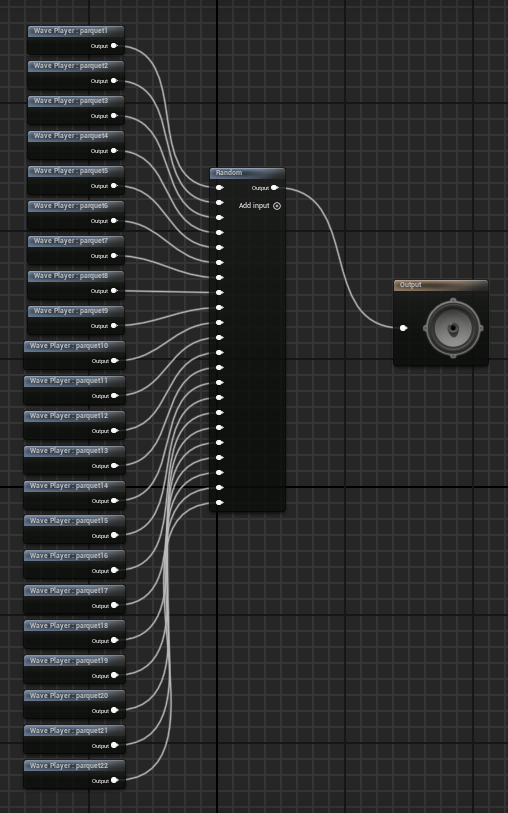
\includegraphics[width=\linewidth, height=6cm]{continut/capitol3/figuri/step_wood.png}
        \label{fig:VR_Pawn}
    \end{subfigure}
    \caption{Footsteps}
\end{figure}

Fiecare grup de sunete utilizează o funcție Random care selectează aleatoriu un clip audio din listă, asigurând astfel o variabilitate mare a sunetelor redate. Acest mecanism contribuie la o experiență audio mai realistă și mai imersivă, reducând efectul de repetiție și artificialitate.

Pentru redarea corectă a sunetelor de pași, este necesară diferențierea între tipurile de suprafețe pe care actorul se deplasează. Această diferențiere se realizează pe baza materialelor asociate cu obiectele din cadrul mediului virtual.

\begin{figure} [htp] 
\centering 
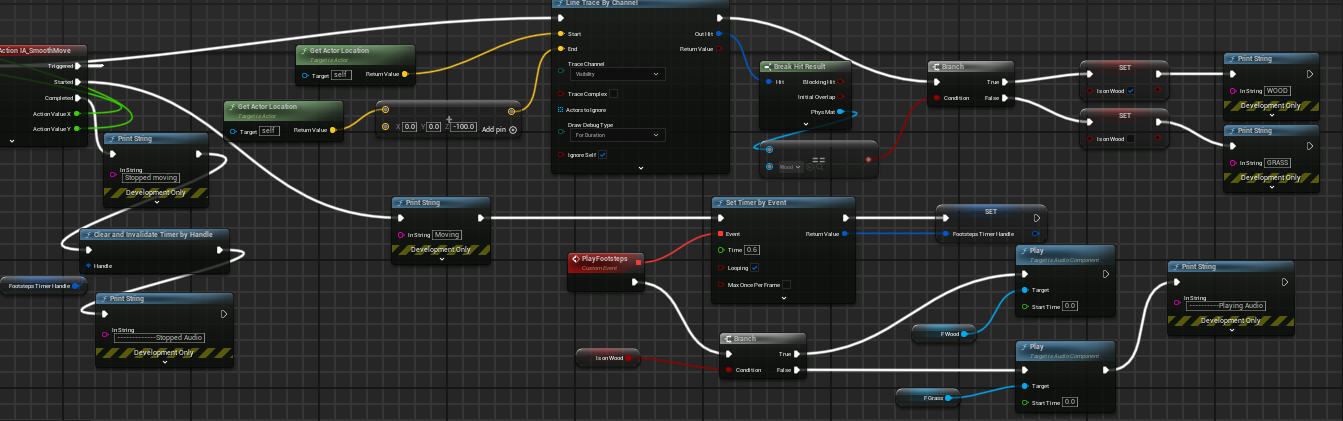
\includegraphics [width=12cm]
{continut/capitol3/figuri/Smooth_Move_Complex.png} 
\label{fig:VR_Pawn} 
    \caption{Smooth Move complet, cu implementarea Phys pentru materiale}
\end{figure}

\textbf{Materiale}

Un material în Unreal Engine poate fi configurat cu o gamă variată de parametri, printre care se numără și atributul „Phys Material”. Acest parametru permite asocierea unui tip specific de material fizic, ce poate fi ulterior identificat în runtime. În cazul aplicației curente, s-au utilizat două tipuri de materiale fizice: „Wood” pentru suprafețele interioare ale muzeului și „Grass” pentru zonele exterioare, unde mediul este natural. Această separare semantică permite sistemului să distingă rapid suprafața pe care se află utilizatorul și să redea sunetul corespunzător.

Pentru a determina materialul pe care se află actorul în orice moment, s-a implementat un sistem de detecție automată a suprafeței. Acesta funcționează pe baza unei raze virtuale (line trace) care este lansată vertical, de sub actor în jos. Mai exact, se folosește funcția LineTraceByChannel, care primește ca parametru poziția actuală a actorului (prin GetActorLocation) pentru a stabili punctul de pornire al razei. Capătul razei este setat la o distanță de 100 de unități sub actor, asigurând astfel detecția obiectului imediat aflat sub picioare.

\begin{figure}[h!]
    \centering
    \begin{subfigure}{0.49\textwidth}
        \includegraphics[width=\linewidth, height=6cm]{continut/capitol3/figuri/phys.png}
        \label{fig:Materials}
    \end{subfigure}
    \hfill
    \begin{subfigure}{0.49\textwidth}
        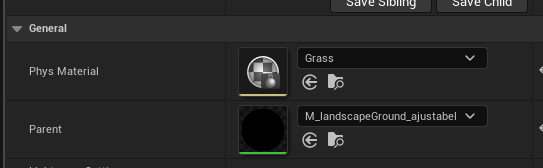
\includegraphics[width=\linewidth, height=6cm]{continut/capitol3/figuri/phys_apply.png}
        \label{fig:Materials}
    \end{subfigure}
    \caption{Aplicatea Phys la fiecare material folosit}
\end{figure}

Această rază de detecție poate fi observată în modul de debugging vizual, dar nu va fi vizibilă în experiența finală pentru utilizator. După lansarea razei, se folosește funcția BreakHitResult pentru a analiza rezultatul coliziunii. Dacă un obiect este detectat, se verifică materialul fizic asociat acestuia, iar în funcție de rezultat se setează o variabilă booleană numită IsOnWood. Aceasta va avea valoarea TRUE dacă suprafața detectată este de tip „Wood” sau FALSE în orice alt caz. În acest mod, putem controla ce tip de sunet va fi redat la fiecare pas, în funcție de contextul în care se află utilizatorul.

Pentru gestionarea redării sunetelor, în momentul în care joystick-ul este înclinat și actorul începe să se deplaseze, este pornit un cronometru intern utilizând funcția SetTimerByEvent. 

Acest cronometru determină intervalul la care vor fi redate sunetele de pași. În funcție de starea variabilei IsOnWood, sistemul va selecta un sunet din setul GrassCore (pentru exterior) sau ParquetCore (pentru interior). Fiecare sunet este selectat aleatoriu dintr-un set de înregistrări, oferind varietate auditivă și realism acustic.

Când joystick-ul nu mai este înclinat (utilizatorul nu mai înaintează), cronometrul este oprit și resetat cu ajutorul funcției ClearAndInvalidateTimerByHandle, prevenind astfel redarea nejustificată a sunetelor între secvențele de deplasare. Acest mecanism contribuie la o experiență sonoră coerentă, adaptată contextului și comportamentului utilizatorului în mediul virtual.

\textbf{SmoothTurn}

Pentru rotația actorului într-un mod fluid și natural, s-a implementat o funcție simplificată, denumită SmoothTurn. Atunci când joystick-ul de pe maneta dreaptă este înclinat spre stânga sau dreapta, este declanșată o actualizare incrementală a orientării actorului. Aceasta se realizează prin funcția AddActorWorldRotation, care modifică rotația actorului pe axa verticală (Yaw) în pași mici și constanți, proporțional cu intensitatea semnalului joystick-ului.

Deși rotația poate fi realizată și fizic de către utilizator prin întoarcerea corpului, această funcționalitate a fost păstrată pentru situațiile în care spațiul fizic disponibil este restricționat (de exemplu, în cazul utilizatorilor care stau pe loc sau folosesc un sistem de tip standing VR).

În cadrul noului sistem de locomoție continuă, direcția de deplasare înainte este influențată direct de orientarea actorului, mai precis de direcția de privire a utilizatorului. Acest aspect este esențial pentru o experiență VR naturală: atunci când utilizatorul își rotește capul, iar comanda joystick-ului rămâne aceeași (spre exemplu, mișcare înainte), deplasarea se va produce în noua direcție a privirii, nu într-o direcție absolută față de scenă. Astfel, mișcarea este întotdeauna contextuală și raportată la orientarea corporală, ceea ce contribuie la o navigare intuitivă în mediul virtual.

Pentru obținerea unui rezultat cât mai confortabil și realist, au fost efectuate numeroase teste de reglaj fin asupra parametrilor ce determină viteza de deplasare și viteza de rotație. Valorile finale au fost alese astfel încât să ofere o experiență fluentă, dar și să prevină apariția simptomelor de disconfort, precum motion sickness sau cybersickness.

\begin{figure} [htp] 
\centering 
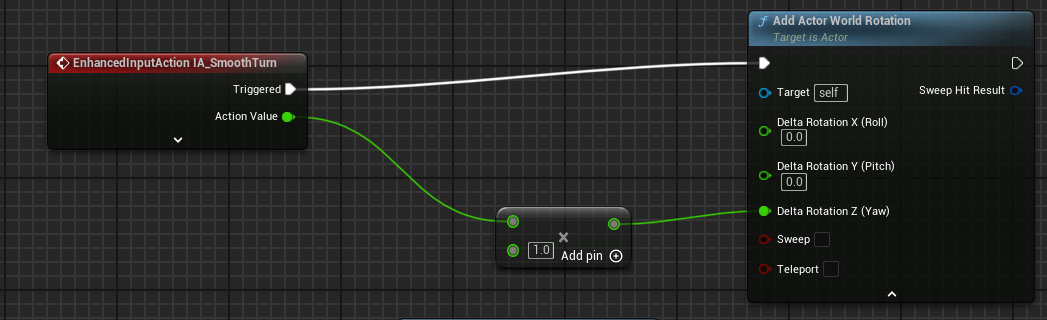
\includegraphics [width=12cm]
{continut/capitol3/figuri/SmoothTurn.png} 
\label{fig:Smooth_Turn} 
    \caption{Smooth Turn}
\end{figure}

\textbf{SmoothTurn}

Un aspect important al designului locomotiei VR este legat de rotația artificială. Deoarece mișcările bruște de rotație pot provoca stări de rău utilizatorilor sensibili, viteza de rotație a fost redusă semnificativ, pentru a permite o adaptare mai blândă a sistemului vizual. Totodată, rotația nu este obligatorie, deoarece utilizatorul se poate întoarce natural în realitate, folosind mișcarea fizică a corpului (în funcție de gradul de libertate oferit de spațiul disponibil în locație). Prin urmare, rotația continuă este oferită ca o opțiune complementară, nu ca un mecanism principal.

Această abordare echilibrată între realism și confort a fost esențială în contextul proiectului VR Museum, unde explorarea spațiului este un element cheie care trebuie să se desfășoare într-un mod accesibil pentru toate categoriile de utilizatori.


\section{Meniul principal și cel de setări}

Meniul de setări din cadrul aplicației VR Museum permite utilizatorului să ajusteze parametrii grafici în funcție de configurația sistemului utilizat, precum și alte opțiuni relevante pentru performanță și confort în realitate virtuală.
Utilizatorul poate selecta unul dintre profilurile grafice prestabilite: Low, Medium, High, Ultra și Cinematic. Deși Unreal Engine permite configurarea detaliată a fiecărui parametru individual, în cadrul aplicației a fost implementată o soluție unificată. Astfel, la alegerea unui profil, toate setările grafice sunt aplicate automat într-o configurație specifică acelui nivel.

Parametrii influențați includ:

\begin{itemize}
\item \textbf{View Distance} - controlează distanța până la care obiectele păstrează modelul 3D complet, înainte de a fi simplificate prin tehnici LOD (Level of Detail).
\item \textbf{Anti-Aliasing} - netezește marginile obiectelor pentru a elimina efectele de tip „jagged edges”.
\item \textbf{Post Processing} - gestionează efectele vizuale aplicate în faza finală de randare, precum:
\begin{center}
\begin{tabular}{||c c||} 
 \hline
 Tehnică & Explicație \\ [0.5ex] 
 \hline\hline
 Ambient Occlusion & calculează umbrirea indirectă între obiecte \\ 
 \hline
 Depth of Field & estompează elementele aflate în afara planului de focus \\
 \hline
 Motion Blur & adaugă estompare obiectelor aflate în mișcare rapidă \\
 \hline
 High Intensity Color & crește saturația imaginii, oferind un efect stilizat  \\ [1ex] 
 \hline
 Chromatic Aberration & simulează aberația cromatică de pe lentile  \\ [1ex] 
 \hline
 Grain & adaugă zgomot vizual pentru un efect cinematic  \\ [1ex] 
 \hline
 Vignette & întunecă subtil marginile cadrului  \\ [1ex] 
 \hline
\end{tabular}
\end{center}

\item \textbf{Shadows} - influențează calitatea și claritatea umbrelor din scenă.
\item \textbf{Global Illumination} - simulează iluminarea indirectă, similar cu Ray Tracing, dar cu un cost computațional mai redus.
\item \textbf{Reflections} - utilizează Lumen, Ray Tracing sau Screen Space Reflections pentru simularea reflexiilor realiste.
\item \textbf{Textures} - reglează rezoluția texturilor aplicate obiectelor, influențând claritatea vizuală și utilizarea memoriei video.
\item \textbf{Effects} - ajustează complexitatea efectelor speciale (particule, volumetrie, transparențe), cu un impact limitat în cadrul aplicației.
\item \textbf{Foliage} - controlează nivelul de detaliu al vegetației, inclusiv comportamentul dinamic în condiții de mediu (vânt, apă).

\end{itemize}

Crearea meniului a implicat mai multe etape: design vizual adaptat pentru VR, scalare în funcție de câmpul vizual și implementarea logicii funcționale. Meniul este apelat printr-un buton de pe controlerele VR și apare în fața utilizatorului, în funcție de direcția privirii la momentul activării. Dacă meniul este deja afișat, o nouă apăsare îl închide, iar o altă activare îl reafișează într-o nouă poziție, actualizată.

\begin{figure}[h!]
    \centering
    \begin{subfigure}{0.49\textwidth}
        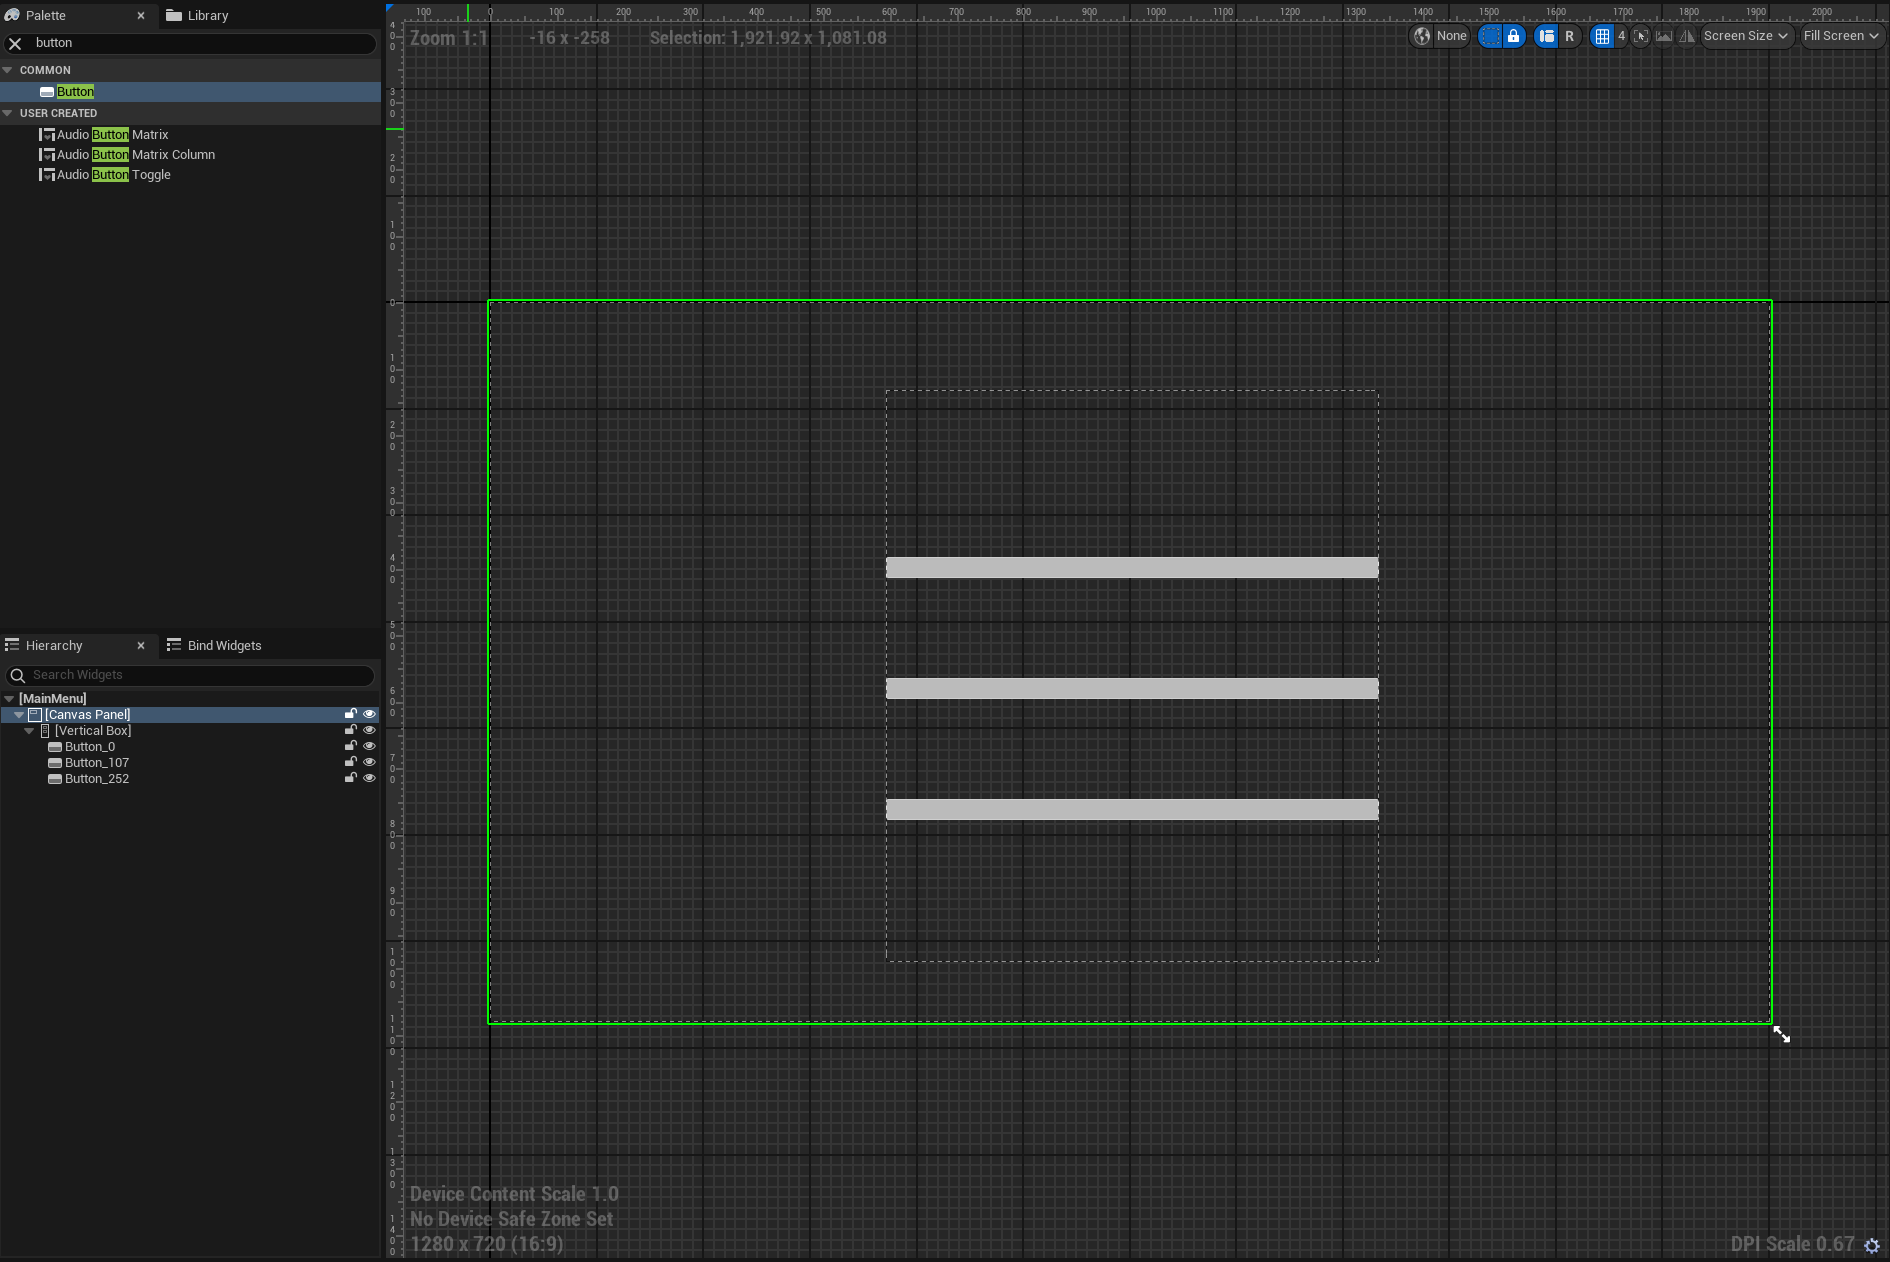
\includegraphics[width=\linewidth, height=6cm]{continut/capitol3/figuri/main_menu_1.png}
        \label{fig:Menu}
    \end{subfigure}
    \hfill
    \begin{subfigure}{0.49\textwidth}
        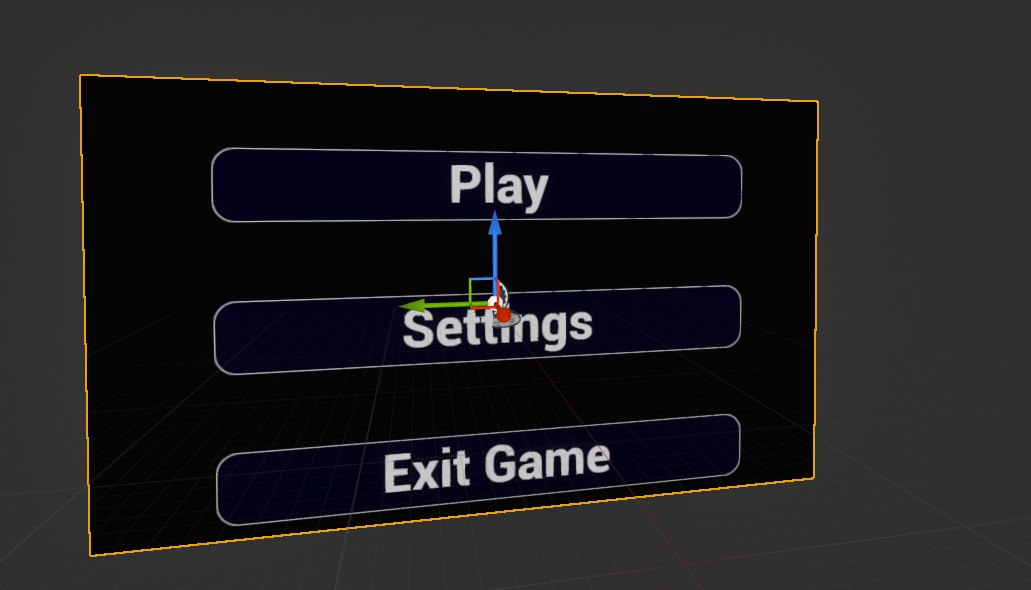
\includegraphics[width=\linewidth, height=6cm]{continut/capitol3/figuri/menu4.png}
        \label{fig:Menu}
    \end{subfigure}
    \caption{Meniul principal - etape din procesul de dezvoltare}
\end{figure}

Cât timp meniul este vizibil, din fiecare mână virtuală se proiectează o linie de ghidare, care permite o selecție ușoară a opțiunilor. Interacțiunea cu butoanele se realizează printr-un sistem de tip OnClick, similar clicurilor de mouse, funcțional atât în UI 2D, cât și în VR.

\begin{figure} [htp] 
\centering 
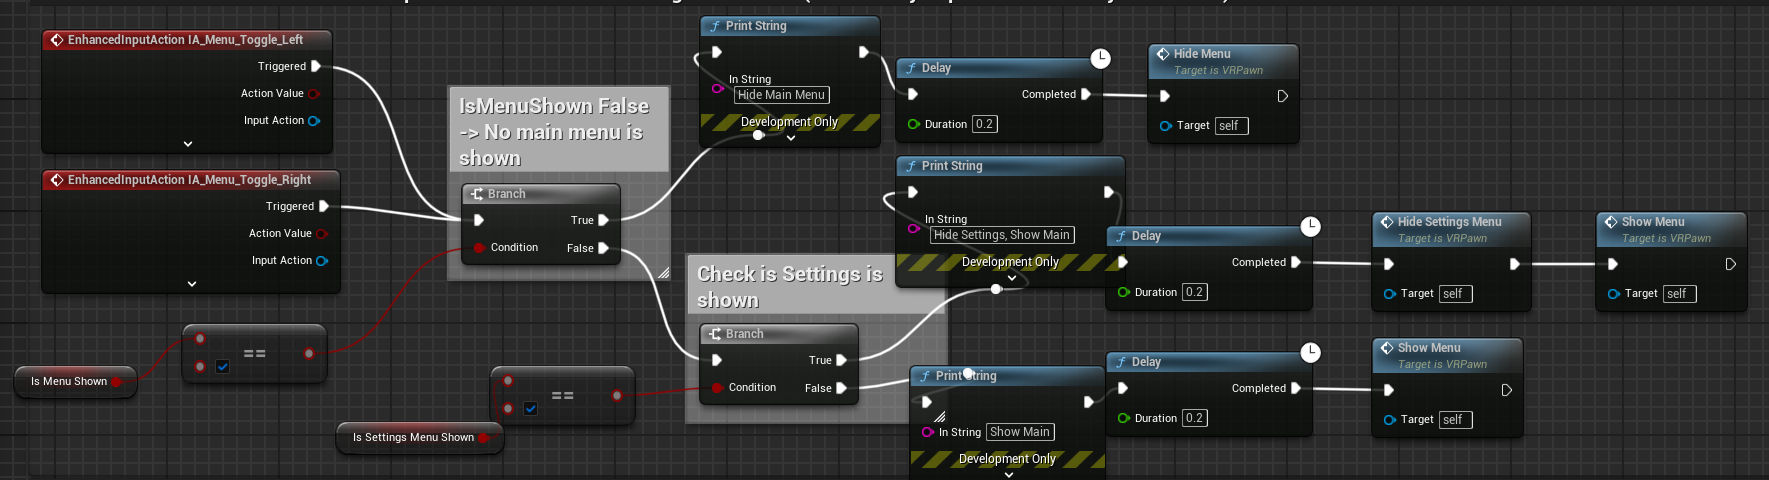
\includegraphics [width=14cm]
{continut/capitol3/figuri/Main_show.png} 
\label{fig:Menu} 
    \caption{Codul responsabil pentru afișarea meniului (prezent in VR Pawn Blueprint)}
\end{figure}
\newpage
Structura meniului principal include următoarele opțiuni:
\begin{itemize}
    \item \textbf{Resume} - închide meniul și permite revenirea în experiența VR;
    \item \textbf{Settings} - închide meniul principal și încarcă meniul de setări;
    \item \textbf{Exit Game} - închide aplicația fără salvarea progresului sau a poziției utilizatorului.
\end{itemize}

\begin{figure} [htp] 
\centering 
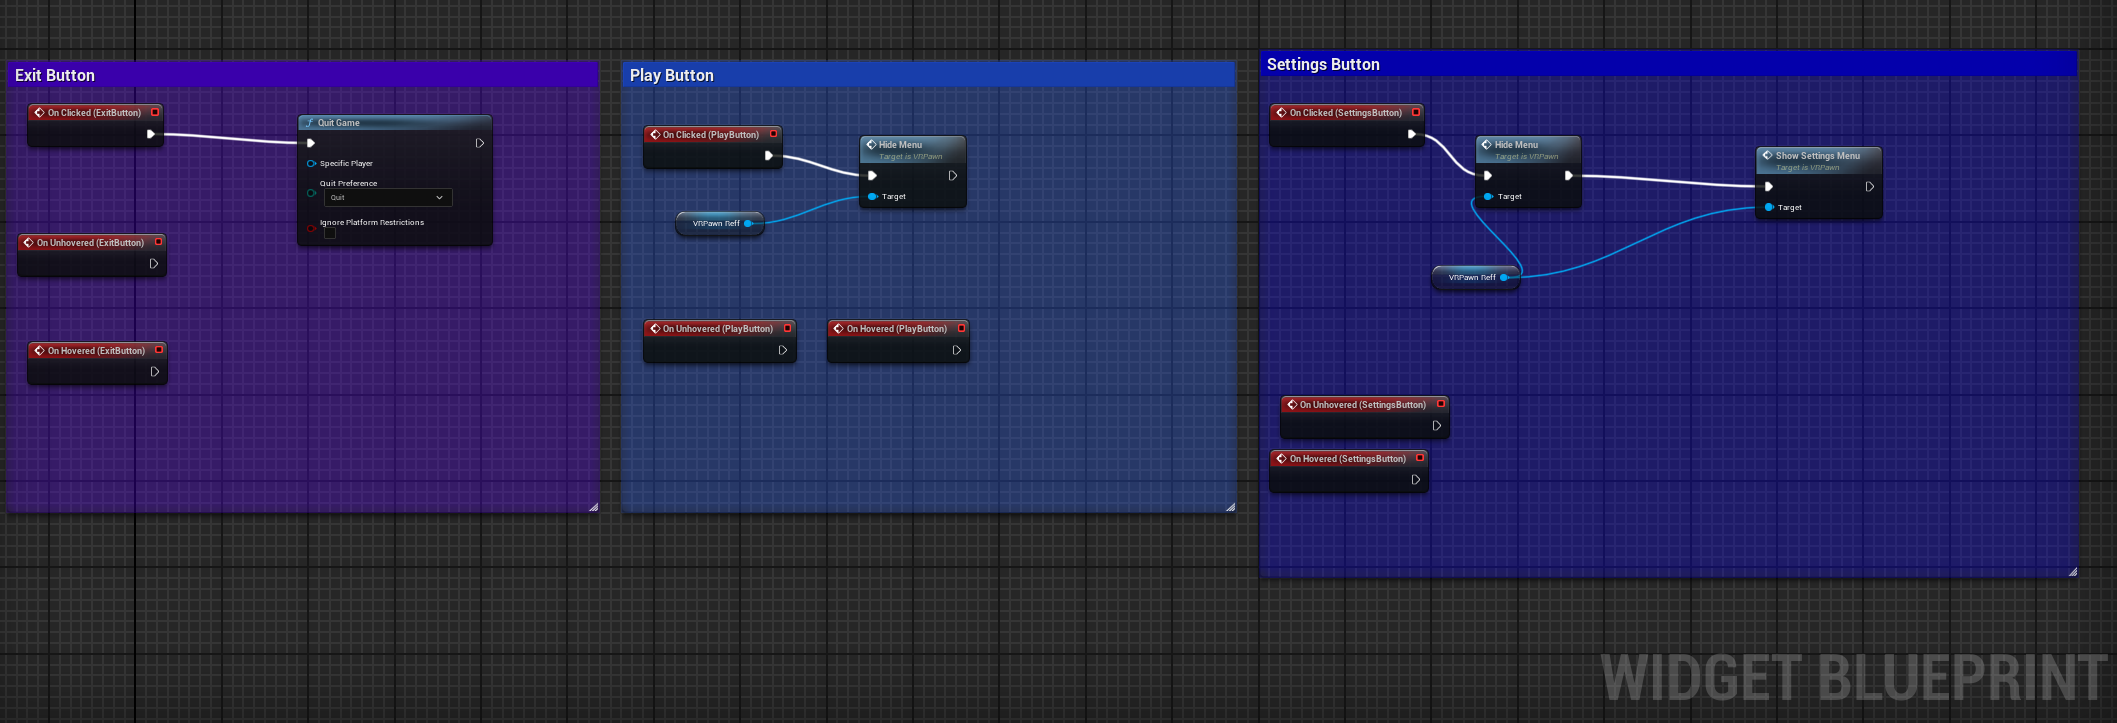
\includegraphics [width=14cm]
{continut/capitol3/figuri/Main_menu_graph.png} 
\label{fig:Menu} 
    \caption{Sectiune din cod ce asigură funcționalitatea butoanelor în meniu}
\end{figure}

\begin{figure} [htp] 
\centering 
\includegraphics [width=14cm]
{continut/capitol3/figuri/ClickSim.png} 
\label{fig:Menu}  
    \caption{Simularea click-ului la apăsarea trigger-ului pe manetele consolei VR}
\end{figure}

Meniul de setări poate fi accesat doar din meniul principal. Acesta include:
\begin{itemize}
    \item \textbf{Graphics} - permite selectarea nivelului general de detaliu vizual;
    \item \textbf{FPS} - stabilește limita de cadre pe secundă;
    \item \textbf{DLSS} - activează sau dezactivează tehnologia de upscaling DLSS;
    \item \textbf{DLSS Settings} - oferă opțiuni suplimentare de configurare a DLSS (Quality, Balanced, Performance).
\end{itemize}


În partea inferioară a meniului sunt plasate două butoane suplimentare:
\begin{itemize}
\item \textbf{Exit} - închide meniul de setări și readuce în scenă meniul principal;
\item \textbf{Apply} - aplică setările selectate, apelând funcțiile specifice fiecărui parametru.
\end{itemize}


\newpage

\begin{figure}[h!]
    \centering
    \begin{subfigure}{0.49\textwidth}
        \includegraphics[width=\linewidth, height=6cm]{continut/capitol3/figuri/settings2.png}
        \label{fig:Menu}
    \end{subfigure}
    \hfill
    \begin{subfigure}{0.49\textwidth}
        \includegraphics[width=\linewidth, height=6cm]{continut/capitol3/figuri/settings3.png}
        \label{fig:Menu}
    \end{subfigure}
    \caption{Meniul de setări - etape din procesul de dezvoltare}
\end{figure}

Selectarea opțiunilor se face prin apăsarea butoanelor dedicate. Butonul selectat este evidențiat vizual printr-o schimbare de culoare, iar sistemul permite activarea unui singur buton pe fiecare linie. Această restricție este gestionată de o logică internă, implementată pentru a preveni conflictele și a menține consistența interfeței.

\begin{figure} [htp] 
\centering 
\includegraphics [width=14cm]
{continut/capitol3/figuri/Settings_graph.png} 
\label{fig:Menu}  
    \caption{Asigurarea apăsării unui singur buton pe linie, cât si aplicarea funcțiilor de schimbare de grafici}
\end{figure}

Este important ca utilizatorii să evite modificarea agresivă a setărilor grafice atunci când aplicația rulează pe sisteme cu resurse limitate, pentru a preveni blocaje sau întreruperi de tip crash.

\begin{figure} [htp] 
\centering 
\includegraphics [width=14cm]
{continut/capitol3/figuri/Graphics.png} 
\label{fig:Menu}  
    \caption{Schimbarea setărilor grafice se face manual, prin comenzi rulate local, pentru fiecare din opțiunile menționate anterior.}
\end{figure} 
\begin{figure} [htp] 
\centering 
\includegraphics [width=14cm]
{continut/capitol3/figuri/FPS.png} 
\label{fig:Menu}  
    \caption{Setarea numărului de cadre secunde se realizează prin executarea comenzii t.maxfps [x], unde x este numărul dorit}
\end{figure}
\begin{figure} [htp] 
\centering 
\includegraphics [width=14cm]
{continut/capitol3/figuri/NvidiaPlugin.png} 
\label{fig:Menu}  
    \caption{Folosirea extensiilor realizare de Nvidia pentru tehnici avansate de upscaling}
\end{figure}
\begin{figure} [htp] 
\centering 
\includegraphics [width=14cm]
{continut/capitol3/figuri/DLSS.png} 
\label{fig:Menu}  
    \caption{Cu ajutorul plugin-urilor furnizate de Nvidia, comenzile precum r.NGX.DLSS.Enable devin accesibile}
\end{figure}
\begin{figure} [htp] 
\centering 
\includegraphics [width=14cm]
{continut/capitol3/figuri/DLSS_Quality.png} 
\label{fig:Menu}  
    \caption{Reglarea rezoluției interne pentru aplicarea unei opțiuni de upscaling}
\end{figure}
\newpage




\section{Cerințele utilizatorului final}

Utilizatorii finali ai aplicației VR Museum sunt persoane interesate de cunoaștere, curioase să exploreze un spațiu cultural într-un mod modern și accesibil. Fie că vorbim despre elevi, studenți, cadre didactice sau persoane pasionate de știință, așteptările acestora se axează pe trei direcții majore: ușurința în utilizare, valoarea educațională a conținutului și imersiunea oferită de experiența VR.

Din punct de vedere al folosirii, VR Museum are un grad scăzut de complexitate, datorită instrucțiunilor incluse în experiența virtuală. Setările pot fi accesate cu ușurință prin apăsarea butoanelor de pe controlerele VR, fie pe cel din mâna dreaptă, fie pe cel din stânga, iar navigarea se realizează simplu și intuitiv cu ajutorul joystick-ului.

Atmosfera trăită în VR Museum este una plăcută și memorabilă; muzeul virtual reușește să redea senzația unui spațiu fizic real, cu o iluminare dinamică adaptată cadrului, sunete ambientale discrete și plăcute, precum și un nivel de detaliu grafic ridicat care contribuie semnificativ la senzația de imersiune.

Aplicația rulează fluent pe majoritatea sistemelor compatibile cu VR. Desigur, nivelul detaliilor vizuale poate varia în funcție de specificațiile tehnice ale echipamentului folosit, însă experiența generală rămâne constantă și de calitate, indiferent de configurație.

Utilizatorii s-ar putea aștepta ca o astfel de aplicație să fie disponibilă contra cost, având în vedere efortul de dezvoltare și numărul mare de ore de muncă investite. Cu toate acestea, VR Museum este oferită gratuit, în format open-source, pentru a putea fi utilizată și extinsă liber în scopuri educaționale, demonstrative sau culturale. Codul sursă este accesibil, permițând dezvoltatorilor să adauge noi funcționalități, să îmbunătățească interfața sau să creeze versiuni personalizate ale muzeului în funcție de propriile nevoi.
    \cleardoublepage

   % \chapter{Testarea aplicației și rezultate experimentale}
\label{cap:cap4}

(aproximativ 7 pagini)

\begin{itemize}
    \item Punerea în funcțiune/lansarea aplicației,elemente de configurare sau instalare;
    \item Testarea sistemului (hardware/software);
    \item Aspecte legate de încărcarea procesorului, memoriei, limitări în ce privește transmisia datelor/comunicarea;
    \item Se prezintă datele de test/metrici/benchmarks
    \item Aspecte legate de fiabilitate/securitate/scalabilitate;
    \item Rezultate experimentale (grafice, tabele, etc.);
    \item Utilizarea sistemului. 
\end{itemize}

\section{Nivel 1}
\label{cap:cap4:nivel1}

\textcolor{gray}{\lipsum}  (Figura \ref{fig:clone_trooper})

\begin{figure}[H]
    \centering
    \includegraphics[width=0.3\textwidth]{continut/capitol4/figuri/clone_trooper.png}
    \caption{Clone Trooper\protect\footnotemark}
    \label{fig:clone_trooper}
\end{figure}
\footnotetext{imagine preluată de pe un site web care nu „merită” trecut la bibliografie \url{https://www.pngitem.com/}}

Tabelul \ref{tabel:tab_simplu} prezintă un exemplu foarte simplu de tabel în \LaTeX. Un alt exemplu este prezentat în Tabelul \ref{tabel:2} din \ref{anexa3:func_xyz}.

\begin{table}[ht]
    \centering
    \caption{Exemplu de tabel simplu}
    \label{tabel:tab_simplu}
    \begin{tabular}{||c l c r||} 
        \hline
        \textbf{Col1} & \textbf{Col2} & \textbf{Col3} & \textbf{Col4} \\
        \hline\hline
        1 & 6 & 87837 & 787 \\ 
        2 & 7 & 78 & 5415 \\
        3 & 545 & 778 & 7507 \\
        4 & 545 & 18744 & 7560 \\
        5 & 88 & 788 & 6344 \\
        \hline
    \end{tabular}
\end{table}

\subsection{Nivel 2}
\label{cap:cap4:nivel1:nivel2}

\subsubsection{Nivel 3}
\label{cap:cap4:nivel1:nivel2:nivel3}

\textcolor{gray}{\lipsum}

\textcolor{gray}{\lipsum}

\textcolor{gray}{\lipsum}

    %\cleardoublepage

    %\chapter{Concluzii}
\label{cap:cap5}

Concluziile lucrării (1–2 pagini) în care se regăsesc cele mai importante concluzii din lucrare, care pornind de la obiectivele propuse în introducerea lucrării vor conține opinia personală a autorului privind rezultatele obținute în lucrare, o comparație a acestora cu alte proiecte/produse similare precum și posibile direcții de dezvoltare. 

\begin{itemize}
    \item Gradul în care s-a realizat tema propusă (motivarea eventualelor obiective modificate);
    \item Evidențierea concisă a contribuțiilor/soluțiilor personale (dacă este cazul);
    \item Comparație cu alte proiecte similare;
    \item Posibile direcții de dezvoltare.
\end{itemize}

În acest capitol nu se introduc figuri, table sau listing-uri de cod. Pot fi în schimb referite!

Concluziile finale au un rol semnificativ în cadrul lucrării de diplomă, care trebuie pus în evidență în special în momentul susținerii acesteia în fața comisiei. Aici trebuie prezentate, în câteva pagini, cele mai importante rezultate ale muncii depuse de candidat și potențiale direcții de dezvoltare ulterioară a temei abordate. Acest capitol oferă o sinteză a realizărilor obținute, precum și avantajele și neajunsurile soluțiilor alese. Concluziile nu trebuie să aducă rezultate sau interpretări noi, ci doar să le evidențieze pe cele din conținutul lucrării.

\section{Direcții viitoare de dezvoltare}
\label{cap:cap5:directii-viitoare}

\textcolor{gray}{\lipsum[1-3]}

\section{Lecții învățate pe parcursul dezvoltării proiectului de diplomă}

Ar fi interesant dacă acest capitol s-ar încheia cu o astfel de secțiune, în mod special la licență.

\textcolor{gray}{\lipsum[2-4]}
    %\cleardoublepage
    % *************** referinte bibliografice ***************
    \bibliographystyle{IEEEtran}
    \bibliography{bibliografie/bibliografie}
    \cleardoublepage
    
    % *************** anexe ***************
    %% config anexe
    % %% refacem counter-ul de figuri/tabele/listing-uri, pentru a putea mentine
%% numerotarea si referirea corecta a figurilor din anexe
\setcounter{figure}{0}
\renewcommand{\thefigure}{A.\arabic{figure}}
\setcounter{table}{0}
\renewcommand{\thetable}{A.\arabic{table}}
%% reset counter capitole, sectiuni pentru anexe
\setcounter{chapter}{0}
\setcounter{section}{0}
\renewcommand{\thesection}{\arabic{section}}
%% titlul anexei in pagina
%% in cuprins va aparea doar numerotat
\titleformat
    {\section}
    [hang]
    {\color{albastru-ac}\bfseries\itshape}
    {Anexa \thesection.\ }
    {0pt}
    {}
    []
    % \silentchapter{Anexe}
%% Nu se pot face referinte pe silentchapter => nu are sens sa pun label
% \label{cap:anexe}

Anexe prezintă doar elementele specifice proiectului!

Anexele (dacă este cazul) constituie o secțiune separată a lucrării care nu se numerotează ca și capitol. Anexele se numerotează crescător cu numere arabe (ex.: Anexa 1, Anexa 2 etc.). Anexele vor conține scheme, diagrame, secvențe din codul sursă.

\section{Componente Software}
\label{anexa1:comp_soft}

% \textit{Componente software:}
\begin{itemize}
    \item diagramele UML care referă numai la componentele dezvoltate de student și care datorită complexității pot fi listate pe o foaie de tip A3 sau A2.
    \item cod sursă numai pentru componentele dezvoltate de către student.
\end{itemize}

%% inserati \newpage inaintea fiecarui \section cu anexa pentru ca fiecare anexa sa inceapa pe pagina noua
\newpage
\section{Componente Hardware}
\label{anexa2:comp_hard}

% \textit{Componente Hardware:}
\begin{itemize}
    \item schemele electrice finale realizate într-un CAD de profil; 
    \item schemele cablajelor realizate pentru implementare, realizate într-un CAD de profil;
    \item informații suplimentare despre implementarea și testarea aplicației (de ex. capturi de osciloscop);
    \item schemele standard ce vor fi folosite pentru testare (pseudocod sau schemă logică);
    \item extrase din foi de catalog. 
\end{itemize}

%% inserati \newpage inaintea fiecarui \section cu anexa pentru ca fiecare anexa sa inceapa pe pagina noua
\newpage
\section{Codul funcției xyz()}
\label{anexa3:func_xyz}

În Figura \ref{fig:AT} este prezentat unul dintre cele mai impunătoare vechicule ale Imperiului.

\begin{figure}[H]
    \centering
    \includegraphics[width=0.5\textwidth]{anexe/figuri/AT.png}
    \caption{AT\protect\footnotemark}
    \label{fig:AT}
\end{figure}
\footnotetext{imagine preluată de pe un site web care nu „merită” trecut la bibliografie \url{https://www.pngitem.com/}}

\textcolor{gray}{\lipsum} (Figura \ref{fig:millennium_falcon})

\begin{figure}[H]
    \centering
    \includegraphics[width=0.8\textwidth]{anexe/figuri/millennium_falcon.jpeg}
    \caption{Millennium Falcon\protect\footnotemark}
    \label{fig:millennium_falcon}
\end{figure}
\footnotetext{imagine preluată de pe un site web care nu „merită” trecut la bibliografie \url{http://clipart-library.com/}}

%% inserati \newpage inaintea fiecarui \section cu anexa pentru ca fiecare anexa sa inceapa pe pagina noua
\newpage
\section{Tabel lung pe mai multe pagini}
\label{anexa4:long_table}

Malware (software rău intenționat) este un termen folosit pentru a descrie orice program sau cod care ocolește procesele de control al accesului, este creat cu intenția de a ataca un sistem de calcul sau rețea, pentru a provoca daune sau a compromite acel sistem. În categoria malware se includ: viruși, \textit{ransomware}, \textit{keyloggers}, troieni, viermi, \textit{spyware} etc (Tabelul \ref{tab_tipuri_de_malware}). În vocabularul curent, termenul de "virus" este folosit abuziv pentru orice tip de malware.

\begin{longtable}[c]{|l|p{7cm}|p{2cm}|}
	\caption{Tipuri de malware\label{tab_tipuri_de_malware}}\\
	
	\hline
	\multicolumn{1}{|c|}{\textbf{\textit{Tip}}} & 
	\multicolumn{1}{c}{\textbf{\textit{Descriere}}} & 
	\multicolumn{1}{|c|}{\textbf{\textit{Exemple elocvente}}}  \\
	\hline
	\endfirsthead
	
	% \multicolumn{3}{c}{Continuarea tabelului \ref{tab_tipuri_de_malware}}\\
	\hline
	\multicolumn{1}{|c|}{\textbf{\textit{Tip}}} & 
	\multicolumn{1}{c}{\textbf{\textit{Descriere}}} & 
	\multicolumn{1}{|c|}{\textbf{\textit{Exemple elocvente}}}  \\
	\hline
	\endhead
	
	\hline
	\endfoot
	
	\hline
	\endlastfoot
	
	\multirow{8}*{Virus} &
	cod executabil malițios, atașat la fișiere sau programe legitime. Majoritatea virușilor necesită declanșarea de către utilizatorul final. Se răspândește prin intermediul unităților USB, discurilor optice, partajărilor în rețea sau e-mail-ului &
	%\multirow{6}*{Brain, Michelangelo, Melissa} \\  
	Brain, \newline Michelangelo, \newline Melissa \\
	\hline

	\multirow{5}{*}{Ransomware} & 
	conceput pentru a ține captiv un sistem informatic, de obicei prin criptarea datelor esențiale, dezactivează accesul victimei la date până la efectuarea unei plăți către atacator & 
	%\multirow{5}{*}{WannaCry, Petya} \\ 
	WannaCry, \newline Petya \\	
	\hline
	
	\multirow{2}{*}{Fileless Malware} & 
	face modificări la fișierele native ale sistemului de operare & 
	\multirow{2}{*}{Astaroth} \\ 
	\hline
	
	\multirow{4}{*}{Spyware} & 
	proiectat pentru a urmări acțiunile utilizatorului și a colecta date despre activitatea victimei, fără cunoștința acesteia & 
	\multirow{4}{*}{DarkHotel} \\ 
	\hline
	
	\multirow{3}{*}{Adware} & 
	livrează anunțuri în mod automat. Unele sunt însoțite de programe \textit{spyware} & 
	\multirow{3}{*}{Fireball} \\ 
	\hline
	
	\multirow{5}{*}{Troian} & 
	execută operațiuni rău intenționate disimulate ca operațiuni dorite. Se deghizează în codul unui program cunoscut și se atașează de fișiere non-executabile & 
	\multirow{5}{*}{Emotet} \\ 
	\hline
	
	\multirow{7}{*}{Worms} & 
	se reproduce singur, se răspândește într-o rețea prin replicare, prin exploatarea vulnerabilităților din rețele. Au tipare similare, inclusiv o vulnerabilitate activă, o modalitate de a se propaga singuri și conțin un \textit{payload} & 
	\multirow{7}{*}{Stuxnet} \\ 
	\hline
	
	\multirow{9}{*}{Rootkit} & 
	conceput pentru a modifica sistemul de operare, astfel încât computerul să poată fi accesat de la distanță, printr-o portiță de acces. Rootkit-urile modifică privilegiile de acces, fișierele de sistem și instrumentele de monitorizare a sistemului, ceea ce le face foarte greu de detectat și eliminat & \multirow{9}{*}{Zacinlo} \\ 
	\hline
	
	\multirow{2}{*}{Keyloggers} & 
	monitorizează apăsările de taste ale victimei & 
	\multirow{2}{*}{Olympic Vision} \\ 
	\hline
	
	\multirow{3}{*}{Bots} & 
	lansează automat atacuri concertate si concentrate asupra sistemului țintă & 
	\multirow{3}{*}{Echobot} \\ 
	\hline
	
	\multirow{2}{*}{Mobile Malware} & 
	conțin cod specific (Android, iOS) infectării dispozitivele mobile & 
	\multirow{2}{*}{Triada} \\ 
	\hline	
\end{longtable}

%% inserati \newpage inaintea fiecarui \section cu anexa pentru ca fiecare anexa sa inceapa pe pagina noua
\newpage
\section{Tabel simplu}
\label{anexa5:simple_table}

Pentru a ușura lecturarea lucrării de diplomă recomandăm ca tabelele (dacă nu sunt prea mari) să nu fie împărțite (sparte) pe mai multe pagini.

\begin{table}[ht]
    \centering
    \caption{Rezultatele simulării}
    \begin{tabular}{|c|c|c|} 
        \hline
        \textbf{\textit{Tipul semnalului}} & \textbf{\textit{Durata}} & \textbf{\textit{Randamentul}} \\
        \hline
        sinusoidal & 10s & 99\% \\ 
        \hline
        dreptunghiular & 12s & 81\% \\
        \hline
        triunghiular & 15s & 89\% \\
        \hline
    \end{tabular}
    \label{tabel:2}
\end{table}

În Tabelul \ref{tabel:2} este prezentat un exemplu de formatare pentru un tabel cu cap de tabel orizontal.

%% inserati \newpage inaintea fiecarui \section cu anexa pentru ca fiecare anexa sa inceapa pe pagina noua
\newpage
\section{Cod în python}
\label{anexa6:listing_python}

\begin{code}
    \begin{minted}{python}
        import numpy as np
            
        def incmatrix(genl1,genl2):
            m = len(genl1)
            n = len(genl2)
            M = None #to become the incidence matrix
            VT = np.zeros((n*m,1), int)  #dummy variable
            
            #compute the bitwise xor matrix
            M1 = bitxormatrix(genl1)
            M2 = np.triu(bitxormatrix(genl2),1)
        
            for i in range(m-1):
                for j in range(i+1, m):
                    [r,c] = np.where(M2 == M1[i,j])
                    for k in range(len(r)):
                        VT[(i)*n + r[k]] = 1;
                        VT[(i)*n + c[k]] = 1;
                        VT[(j)*n + r[k]] = 1;
                        VT[(j)*n + c[k]] = 1;
                        
                        if M is None:
                            M = np.copy(VT)
                        else:
                            M = np.concatenate((M, VT), 1)
                        
                        VT = np.zeros((n*m,1), int)
            
            return M
    \end{minted} 
    \caption{Codul funcției \textit{incmatrix}} 
    \label{code:python_incmatrix}
\end{code}

%% inserati \newpage inaintea fiecarui \section cu anexa pentru ca fiecare anexa sa inceapa pe pagina noua
\newpage
\section{Cod în Kotlin (mai lung de o pagină)}
\label{anexa7:listing_kotlin}

\begin{code}
    \begin{minted}{kotlin}
internal inner class ScheduleAdapter : 
        RecyclerView.Adapter<CalendarSessionViewHolder>(),
        StickyHeaderHandler {
        
    private var schedule: MutableList<ScheduleItem> = mutableListOf()
    var data: List<SessionDataGroup> = emptyList()
        set(value) {
            updateSchedule(value)
            field = value
        }

    override fun onCreateViewHolder(
            parent: ViewGroup, 
            viewType: Int): CalendarSessionViewHolder {
        val view = when (viewType) {
            ScheduleItem.TYPE_SMALL ->
                    R.layout.item_schedule_session_header_small
            ScheduleItem.TYPE_LARGE -> 
                    R.layout.item_schedule_session_header_large
            else -> R.layout.item_schedule_session_card
        }

        val holder = layoutInflater.inflate(view, parent, false)
        return CalendarSessionViewHolder(holder, _favoriteNeedSync)
    }
    override fun getItemCount(): Int = schedule.size

    override fun onBindViewHolder(
        holder: CalendarSessionViewHolder, position: Int) {
        holder.show(schedule[position])
    }

    override fun getItemViewType(position: Int): Int {
        return schedule[position].type
    }
    private fun updateSchedule(groups: List<SessionDataGroup>) {
        val result = mutableListOf<ScheduleItem>()
        for (group in groups) {
            if (group.type == 0) {
                result += ScheduleItem.SmallHeader(
                    group.title, R.color.dark_grey_40
                )
                continue
            }
            if (group.type == 1) {
                result += ScheduleItem.LargeHeader(group)
                continue
            }

            result += ScheduleItem.LargeHeader(group)
            result += group.sessions.map { ScheduleItem.Card(it) }
        }

        schedule = result
    }
    override fun getAdapterData(): MutableList<*> = schedule
}
    \end{minted}
    \caption{clasa \textit{ScheduleAdapter}} 
    \label{code:kotlin_scheduleAdapter}
\end{code}

%% inserati \newpage inaintea fiecarui \section cu anexa pentru ca fiecare anexa sa inceapa pe pagina noua
\newpage
\section{Cod în XML (preluat din fisier)}
\label{anexa8:listing_xml}

\begin{code}
    \inputminted{xml}{anexe/coduri_sursa/pom.xml}
    \caption{Exemplu de cod XML preluat din fișier extern}
    \label{code:xml_pom}
\end{code}



    % \cleardoublepage

\end{document}
